\documentclass[9pt]{beamer}
%\usetheme[pageofpages=of]{Singapore}
\usetheme[titleformat frame = smallcaps]{metropolis}
%\usepackage{FiraSans}
\usepackage{FiraMono}
%\usecolortheme{freewilly}
%\usetheme{Singapore}
\setbeamertemplate{navigation symbols}{}
%\setbeamertemplate{mini frames}{}
%\usetheme{Frankfurt}
%\usefonttheme{professionalfonts}  
%\setbeamertemplate{footline}[frame number]
\usepackage[utf8]{inputenc}
\usepackage[francais]{babel}



%\usepackage{/home/paul/Workspace/build/macros}

\metroset{sectionpage=none}

\setbeamersize{text margin left=5mm,text margin right=5mm} 
%\setbeamersize{text margin left=9mm,text margin right=3mm} 

\setbeamertemplate{section in toc}[sections numbered]


%\setbeamercolor{title}{parent=palette quaternary}
%\setbeamercolor{frametitle}{bg=white, fg=black}
%\setbeamercolor{section in head/foot}{parent=palette quaternary}
%\colorlet{bullet}{red}
%\defbeamertemplate*{mini frame}{Frankfurt}
%{%
%  \begin{pgfpicture}{0pt}{0pt}{0.1cm}{0.1cm}
%    \pgfsetcolor{bullet}% draw and fill in red
%    \pgfsetfillcolor{bullet}% only fill in red
%    \pgfpathcircle{\pgfpoint{0.05cm}{0.05cm}}{0.05cm}
%    \pgfusepath{fill,stroke}
%  \end{pgfpicture}%
%}[action]{ \setbeamersize{mini frame size=.14cm,mini frame offset=.03cm} }

%\usepackage[dvips]{epsfig} 
  

\usepackage[gen]{eurosym}
\usepackage{graphicx}
\usepackage{amssymb}
\usepackage{amsmath}
\usepackage{mathrsfs}
\usepackage{mathdots}
\usepackage{wrapfig}
\usepackage{multirow}
\usepackage{cancel}
\usepackage{pgfplots}
\usepackage{tikz}
\usepackage{etoolbox}
\usetikzlibrary{matrix} % for block alignment
\usetikzlibrary{arrows} % for arrow heads
\usetikzlibrary{calc} % for manimulation of coordinates


\usepackage{pgfplotstable}
\usepackage{mathtools}
\usepackage{etextools}
\usepackage{comment}
\usepackage{bm}
\usepackage{algorithm2e}

\usepackage{stmaryrd}
\usepackage{multicol}

\usepackage[position=bottom]{subfig}

% TikZ styles for drawing
\tikzstyle{block} = [draw,rectangle,thick,minimum height=2em,minimum width=2em]
\tikzstyle{sum} = [draw,circle,inner sep=0mm,minimum size=2mm]
\tikzstyle{connector} = [->,thick]
\tikzstyle{line} = [thick]
\tikzstyle{branch} = [circle,inner sep=0pt,minimum size=1mm,fill=black,draw=black]
\tikzstyle{guide} = []

\RequirePackage{ifthen} % package required


\newcommand{\Blue}[1]{\textcolor{blue}{#1}}
\newcommand{\Red}[1]{\textcolor{red}{#1}}
\newcommand{\Green}[1]{\textcolor{green}{#1}}

\newcommand{\mlprod}[4]{[\![#1;\, #2,#3,#4]\!]}
\newcommand{\cpd}[3]{[\![#1, #2,#3]\!]}

\usepackage{enumitem}
%\renewcommand\labelitemi{---}


%\setbeamertemplate{itemize items}[default]
%\setbeamertemplate{enumerate items}[default]


\def\R{\mathbfhbb{R}}
\def\C{\mathbfhbb{C}}
\def\H{\mathbfhbb{H}}
\def\HC{{\mathbfhbb{H}_\mathbfhbb{C}}}
\def\im{\texttt{i}}
\def\jm{\texttt{j}}
\def\km{\texttt{k}}
%\def\e{\mathbfhrm{e}}
\def\b{\mathbfhbf}
\def\cal{\mathbfhcal}
%\newcommand{\brouge}[1]{\textcolor{br}{#1}}
\newtheorem{theo}{Théorème}

%\makeatletter
%\patchcmd{\@listI}{\itemsep3\p@}{\itemsep1.25em}{}{}
%\makeatother

%\usetheme{Warsaw}


%\usepackage{remreset}% tiny package containing just the \@removefromreset command
%\makeatletter
%\@removefromreset{subsection}{section}
%\makeatother
%\setcounter{subsection}{1}


\def\scrA{\mathscr{A}}
\def\scrB{\mathscr{B}}
\def\scrC{\mathscr{C}}
\def\scrD{\mathscr{D}}
\def\scrE{\mathscr{E}}
\def\scrF{\mathscr{F}}
\def\scrG{\mathscr{G}}
\def\scrH{\mathscr{H}}
\def\scrI{\mathscr{I}}
\def\scrJ{\mathscr{J}}
\def\scrK{\mathscr{K}}
\def\scrL{\mathscr{L}}
\def\scrM{\mathscr{M}}
\def\scrN{\mathscr{N}}
\def\scrO{\mathscr{O}}
\def\scrP{\mathscr{P}}
\def\scrQ{\mathscr{Q}}
\def\scrR{\mathscr{R}}
\def\scrS{\mathscr{S}}
\def\scrT{\mathscr{T}}
\def\scrU{\mathscr{U}}
\def\scrV{\mathscr{V}}
\def\scrW{\mathscr{W}}
\def\scrX{\mathscr{X}}
\def\scrY{\mathscr{Y}}
\def\scrZ{\mathscr{Z}}

\def\calA{\mathcal{A}}
\def\calB{\mathcal{B}}
\def\calC{\mathcal{C}}
\def\calD{\mathcal{D}}
\def\calE{\mathcal{E}}
\def\calF{\mathcal{F}}
\def\calG{\mathcal{G}}
\def\calH{\mathcal{H}}
\def\calI{\mathcal{I}}
\def\calJ{\mathcal{J}}
\def\calK{\mathcal{K}}
\def\calL{\mathcal{L}}
\def\calM{\mathcal{M}}
\def\calN{\mathcal{N}}
\def\calO{\mathcal{O}}
\def\calP{\mathcal{P}}
\def\calQ{\mathcal{Q}}
\def\calR{\mathcal{R}}
\def\calS{\mathcal{S}}
\def\calT{\mathcal{T}}
\def\calU{\mathcal{U}}
\def\calV{\mathcal{V}}
\def\calW{\mathcal{W}}
\def\calX{\mathcal{X}}
\def\calY{\mathcal{Y}}
\def\calZ{\mathcal{Z}}

\def\bfa{\mathbf{a}}
\def\bfb{\mathbf{b}}
\def\bfc{\mathbf{c}}
\def\bfd{\mathbf{d}}
\def\bfe{\mathbf{e}}
\def\bff{\mathbf{f}}
\def\bfg{\mathbf{g}}
\def\bfh{\mathbf{h}}
\def\bfi{\mathbf{i}}
\def\bfj{\mathbf{j}}
\def\bfk{\mathbf{k}}
\def\bfl{\mathbf{l}}
\def\bfm{\mathbf{m}}
\def\bfn{\mathbf{n}}
\def\bfo{\mathbf{o}}
\def\bfp{\mathbf{p}}
\def\bfq{\mathbf{q}}
\def\bfr{\mathbf{r}}
\def\bfs{\mathbf{s}}
\def\bft{\mathbf{t}}
\def\bfu{\mathbf{u}}
\def\bfv{\mathbf{v}}
\def\bfw{\mathbf{w}}
\def\bfx{\mathbf{x}}
\def\bfy{\mathbf{y}}
\def\bfz{\mathbf{z}}

\def\bfA{\mathbf{A}}
\def\bfB{\mathbf{B}}
\def\bfC{\mathbf{C}}
\def\bfD{\mathbf{D}}
\def\bfE{\mathbf{E}}
\def\bfF{\mathbf{F}}
\def\bfG{\mathbf{G}}
\def\bfH{\mathbf{H}}
\def\bfI{\mathbf{I}}
\def\bfJ{\mathbf{J}}
\def\bfK{\mathbf{K}}
\def\bfL{\mathbf{L}}
\def\bfM{\mathbf{M}}
\def\bfN{\mathbf{N}}
\def\bfO{\mathbf{O}}
\def\bfP{\mathbf{P}}
\def\bfQ{\mathbf{Q}}
\def\bfR{\mathbf{R}}
\def\bfS{\mathbf{S}}
\def\bfT{\mathbf{T}}
\def\bfU{\mathbf{U}}
\def\bfV{\mathbf{V}}
\def\bfW{\mathbf{W}}
\def\bfX{\mathbf{X}}
\def\bfY{\mathbf{Y}}
\def\bfZ{\mathbf{Z}}

\def\bfone{\mathbf{1}} % ???
\def\bfzero{\mathbf{0}} % ???

\def\bbA{\mathbb{A}}
\def\bbB{\mathbb{B}}
\def\bbC{\mathbb{C}}
\def\bbD{\mathbb{D}}
\def\bbE{\mathbb{E}}
\def\bbF{\mathbb{F}}
\def\bbG{\mathbb{G}}
\def\bbH{\mathbb{H}}
\def\bbI{\mathbb{I}}
\def\bbJ{\mathbb{J}}
\def\bbK{\mathbb{K}}
\def\bbL{\mathbb{L}}
\def\bbM{\mathbb{M}}
\def\bbN{\mathbb{N}}
\def\bbO{\mathbb{O}}
\def\bbP{\mathbb{P}}
\def\bbQ{\mathbb{Q}}
\def\bbR{\mathbb{R}}
\def\bbS{\mathbb{S}}
\def\bbT{\mathbb{T}}
\def\bbU{\mathbb{U}}
\def\bbV{\mathbb{V}}
\def\bbW{\mathbb{W}}
\def\bbX{\mathbb{X}}
\def\bbY{\mathbb{Y}}
\def\bbZ{\mathbb{Z}}

\def\rmA{\mathrm{A}}
\def\rmB{\mathrm{B}}
\def\rmC{\mathrm{C}}
\def\rmD{\mathrm{D}}
\def\rmE{\mathrm{E}}
\def\rmF{\mathrm{F}}
\def\rmG{\mathrm{G}}
\def\rmH{\mathrm{H}}
\def\rmI{\mathrm{I}}
\def\rmJ{\mathrm{J}}
\def\rmK{\mathrm{K}}
\def\rmL{\mathrm{L}}
\def\rmM{\mathrm{M}}
\def\rmN{\mathrm{N}}
\def\rmO{\mathrm{O}}
\def\rmP{\mathrm{P}}
\def\rmQ{\mathrm{Q}}
\def\rmR{\mathrm{R}}
\def\rmS{\mathrm{S}}
\def\rmT{\mathrm{T}}
\def\rmU{\mathrm{U}}
\def\rmV{\mathrm{V}}
\def\rmW{\mathrm{W}}
\def\rmX{\mathrm{X}}
\def\rmY{\mathrm{Y}}
\def\rmZ{\mathrm{Z}}

\def\rmA{\mathrm{A}}
\def\rmB{\mathrm{B}}
\def\rmC{\mathrm{C}}
\def\rmD{\mathrm{D}}
\def\rmE{\mathrm{E}}
\def\rmF{\mathrm{F}}
\def\rmG{\mathrm{G}}
\def\rmH{\mathrm{H}}
\def\rmI{\mathrm{I}}
\def\rmJ{\mathrm{J}}
\def\rmK{\mathrm{K}}
\def\rmL{\mathrm{L}}
\def\rmM{\mathrm{M}}
\def\rmN{\mathrm{N}}
\def\rmO{\mathrm{O}}
\def\rmP{\mathrm{P}}
\def\rmQ{\mathrm{Q}}
\def\rmR{\mathrm{R}}
\def\rmS{\mathrm{S}}
\def\rmT{\mathrm{T}}
\def\rmU{\mathrm{U}}
\def\rmV{\mathrm{V}}
\def\rmW{\mathrm{W}}
\def\rmX{\mathrm{X}}
\def\rmY{\mathrm{Y}}
\def\rmZ{\mathrm{Z}}
\newcommand{\defeq}{\mathrel{:=}}
\newcommand{\mvec}{\mathop{\text{vec}}}
\newcommand{\rrank}{\mathop{\text{rank}}}
\newcommand{\rowspan}{\mathop{\text{rowspan}}}
\newcommand{\minim}{\mathop{\text{\;minimize\;}}}
\newcommand{\sto}{\mathop{\text{\;subject\ to\;}}}
\newcommand{\diag}{\mathop{\mathrm{diag}}} % ???
\newcommand{\trace}{\mathop{\text{tr}}} % ???
\newcommand{\vcol}{\mathop{\mathrm{col}}} % ???
\def\blkdiag{\mathop{\mathrm{blkdiag}}} % ???
\def\elprod{\odot}
\newcommand{\dist}{\mathop{\text{dist}}}

\newcommand{\bmx}{\begin{bmatrix}}
\newcommand{\emx}{\end{bmatrix}}
\newcommand{\bsm}{\left[\begin{smallmatrix}}
\newcommand{\esm}{\end{smallmatrix}\right]}

\newcommand{\ie}{\emph{i.e.}}
\newcommand{\eg}{\emph{e.g.}}

\newcommand{\imgmap}{\mathop{\mathrm{Img}}}
\newcommand{\bbNz}{\mathbb{N}_0} % ???
\def\bbZp{\mathbb{Z}_{+}}

\def\adj{\mathop{\mathrm{adj}}}%\big(#1\big)}
\def\ddet{\mathop{\mathrm{det}}}%\big(#1\big)}
\def\rowspan{\mathop{\mathrm{rowspan}}}

\def\rowvec#1#2{[\,#1 \; \cdots \; #2\,]}
%\input{slraalgdefs}
% VARIETIES
\newcommand{\var}[1]{\mathcal{#1}} % subspaces


% SETS, SPACES, VARIETIES
\newcommand{\set}[1]{{#1}} % subspaces

% TENSORS
\newcommand{\tens}[1]{\mathcal{#1}}

% ARRAYS OF ORDER>2 (representing tensors in given bases)
\newcommand{\arr}[1]{\mathbf{#1}}

% MATRICES
\newcommand{\matr}[1]{\mathbf{#1}}

% VECTORS
\newcommand{\vect}[1]{\mathbf{#1}} % \boldsymbol{#1} is more beautiful, and works for greek letters
\newcommand{\vx}{\vect{x}}
\newcommand{\vd}{\vect{d}}
\newcommand{\vb}{\vect{b}}

% OPERATORS
\makeatletter
\newcommand{\T}{{\sf T}}      % transposition
\renewcommand{\H}{{\sf H}}      % Hermitian transposition

\newcommand{\krank}[1]{\mathop{\operator@font krank}\{#1\}}
\newcommand{\Diag}[1]{\mathop{\operator@font Diag}\{#1\}}    % a diagonal matrix
%\newcommand{\diag}[1]{\mathop{\operator@font diag}\{#1\}}    % a vector
\newcommand{\Span}[1]{\mathop{\operator@font Span}\{#1\}}    % a space
\renewcommand{\vec}{\mathop{\operator@font vec}} % vectorisation
\newcommand{\codim}[1]{\mathop{\operator@font codim} #1}    % codimension
\makeatother
\newcommand{\out}{\otimes}    % outer (tensor) product
\newcommand{\khatri}{\odot}   % Khatri-Rao product
\newcommand{\hadam}{\boxdot}  % Hadamard product
\newcommand{\kron}{\boxtimes}  % Kronecker product
\newcommand{\E}{\mathbb{E}}
\newcommand{\Hilbert}{\mathcal{H}}
\newcommand{\Fourier}{\mathcal{F}}
\newcommand{\eqdef}{\stackrel{\mathrm{def}}{=}}
\newcommand{\con}{\mathop{\bullet}} % contraction
% \def\prodmode#1{\times_{#1}} %product along the mode
\newcommand{\prodmode}[1]{\con_{#1}} %product along the mode

% COMMENTS
\newcommand{\KU}[1]{{\color{ForestGreen}{\textbf{KU}:  #1}}}
\newcommand{\YQ}[1]{{\color{blue}{\textbf{YQ}:  #1}}}
\newcommand{\yq}{\color{blue}}
\newcommand{\PC}[1]{{\color{BrickRed}{\textbf{PC}: #1}}}
\definecolor{darkgreen}{rgb}{0,0.4,0}
\newcommand{\ku}{\color{darkgreen}}
\newcommand{\pc}{\color{BrickRed}}
\newcommand{\fin}{\color{black}}

% LOCAL MACROCOMMANDS
\newcommand{\NN}{\mathbb{N}} % natural numbers
\newcommand{\KK}{\mathbb{F}} % general field
\newcommand{\RR}{\mathbb{R}} % real
\newcommand{\CC}{\mathbb{C}} % complex
\newcommand{\PP}{\mathbb{P}} % projective complex

\newcommand{\form}{T} % symbol for a form
\newcommand{\cumulant}{\mathcal{C}} % cumulant



\providecommand{\sspan}[1]{\operatorname{span}(#1)} % X-rank
\providecommand{\rank}[1]{\operatorname{rank}(#1)} % X-rank
\providecommand{\xrank}[1]{\operatorname{rank}_{X}(#1)} % X-rank

\DeclarePairedDelimiter{\ceil}{\lceil}{\rceil}
\DeclarePairedDelimiter\floor{\lfloor}{\rfloor}
\DeclarePairedDelimiter{\brackets}{[}{]} %used in a lot of math operators
\DeclarePairedDelimiter{\parens}{(}{)} %used in a lot of math operators

\def\hankel#1#2{\mathscr{H}_{#1}\parens{#2})} %product along the mode
\def\sthankel#1#2{\mathscr{S}_{#1}\parens{#2}}

\def\ambspace{\set{A}}
\def\vars{\vect{u}}
\def\varsk#1{u_{#1}}

\def\rGenSdV{\rho}

% Theorem definitions



\newcommand{\abs}[1]{| #1 |}
\newcommand{\norm}[1]{|\!| #1 |\!|}

\DeclareMathOperator{\Tr}{Tr}

\newcommand{\contr}[1]{\mathop{\bullet_{#1}}}   % Contraction
\newtheorem{prop}{Proposition} 

\author{Cours élaboré à partir de cours de D. Brie, S. Miron et K. Usevich \\CRAN, CNRS/Univ. Lorraine  }
\title{Optimisation Numérique et Sciences des Données}
\subtitle{Sciences des Données - Décompositions matricielles}
%\subtitle{r\'{e}union CICS}

\date{Master ISC}

\author{Paul Catala (CRAN, UL) \hfill Master Ingénierie des Systèmes Complexes}
%\date{Postdoctorant à l'université d'Osnabrück, Allemagne}
\date{paul.catala(at)univ-lorraine.fr \hfill Semestre 9 -- 2025 \\ \\ D'après des cours de D. Brie, S. Miron et K. Usevich}

\definecolor{myblue}{RGB}{0,20,225}
\definecolor{myorange}{RGB}{255,196,0}
 \definecolor{darkgreen}{rgb}{0,0.5,0}

\setbeamercolor{bluetext_color}{fg=myblue}
\setbeamercolor{myorange_color}{fg=myorange}
\newcommand{\bluetext}[1]{{\usebeamercolor[fg]{bluetext_color}#1}}
\definecolor{lightgrey}{RGB}{222,222,222}
\definecolor{llightgrey}{RGB}{240,240,240}
\setbeamercolor*{block body}{bg=llightgrey}
\setbeamerfont{headline}{size=\footnotesize}
\setbeamerfont{frame number}{size=\normalsize}
\setbeamerfont{footline}{size=\footnotesize}


\setbeamercolor{background canvas}{bg=white}

%\setbeamercolor*{item}{bg=red, fg=red}

\usefonttheme[onlymath]{serif}

\def\nvar{\mathrm{q}}

%\setbeamercolor*{palette tertiary}{fg=red, bg=black}
%\setbeamercolor*{palette quaternary}{fg=green, bg=black}
%\setbeamercolor*{headline}{bg=black}

\setbeamercolor{section in head/foot}{parent=palette tertiary,fg=blue}
\setbeamertemplate{section in head/foot shaded}{\color{black!20}\usebeamertemplate{section in head/foot}}

\usepackage[skins,theorems]{tcolorbox}
\tcbset{highlight math style={colback=mLightBrown!20,colframe=black!2,sharp corners},bottom=2pt,top=2pt}
\tcbset{left skip={-.01\linewidth}, colback=mLightBrown!20,colframe=black!2,sharp corners,left=0pt,right=0pt}


%\setbeamercolor{section in head/foot}{fg=green, use=red}
%\setbeamercolor{mini frame}{fg=blue, use=drakgray}

%\setbeamercolor{caption name}{fg=green}
%\setbeamercolor{section in toc shaded}{fg=green}

\begin{document}
\newboolean{sectiontoc}
\setboolean{sectiontoc}{true} % default to true

%\AtBeginSection[]
%{
  %\ifthenelse{\boolean{sectiontoc}}{
    %\begin{frame}<beamer>[noframenumbering,plain]{Plan}
      %\tableofcontents[currentsection]
    %\end{frame}
  %}
%}

\newcommand{\toclesssection}[1]{
  \setboolean{sectiontoc}{false}
  \section{#1}
  \setboolean{sectiontoc}{true}
}


\setbeamercolor{section in head/foot}{fg=normal text.bg, bg=structure.fg}



\makeatletter
%\newcommand{\xleftrightarrow}[2][]{\ext@arrow 3359\leftrightarrowfill@{#1}{#2}}
\newcommand{\xdashrightarrow}[2][]{\ext@arrow 0359\rightarrowfill@@{#1}{#2}}
\newcommand{\xdashleftarrow}[2][]{\ext@arrow 3095\leftarrowfill@@{#1}{#2}}
\newcommand{\xdashleftrightarrow}[2][]{\ext@arrow 3359\leftrightarrowfill@@{#1}{#2}}
\def\rightarrowfill@@{\arrowfill@@\relax\relbar\rightarrow}
\def\leftarrowfill@@{\arrowfill@@\leftarrow\relbar\relax}
\def\leftrightarrowfill@@{\arrowfill@@\leftarrow\relbar\rightarrow}
\def\arrowfill@@#1#2#3#4{%
  $\m@th\thickmuskip0mu\medmuskip\thickmuskip\thinmuskip\thickmuskip
   \relax#4#1
   \xleaders\hbox{$#4#2$}\hfill
   #3$%
}
\makeatother


\renewcommand{\nvar}{n}

\begin{frame}[t,plain]
\titlepage
\end{frame}


%\begin{frame}
%\frametitle{A summary}
%
%\vspace{-2em}
%
%\[
%\begin{tikzpicture}[xshift=-1cm]
%\begin{scope}[scale= 0.75]
%     \tikzstyle{block} = [draw,rectangle,thick, rounded corners = 0.4cm,minimum width = 2cm, minimum height=0.8cm]
%     \tikzstyle{sum} = [draw,circle,inner sep=0mm,minimum size=2mm]
%     \tikzstyle{connector} = [->,thick]
%     \tikzstyle{line} = [thick]
%
%
%
%%    \draw (0,-2.7) node[block] (Data1)	{$\begin{array}{@{}c@{}}
%%\mbox{matrix}\\
%%\mbox{factorization} \\
%%\tikz \node [scale=0.3,rounded corners=0pt, color=black] {\begin{tikzpicture}
%%\begin{scope}
%%%\draw(0.6,0.6) node (A) {$\mathcal{T}$};
%%\draw(0,0) rectangle (1.2,1.2);
%%%\draw(0,1) -- (0.5,1.5) -- (1.5,1.5) -- (1.5,0.5) --(1,0);
%%%\draw(1,1) -- (1.5,1.5);
%%
%%\draw(1.7,0.5) node (eq) {\Huge$=$};
%%\draw(2.2,0) rectangle (2.9,1.2); %node {A};
%%%\draw(2.5,0.6) node (A) {$A$};
%%%\draw(5,0.5) node (eq) {\footnotesize$\quad+\,\cdots\,+\quad$};
%%\draw(3.2,0.5) rectangle (4.4,1.2); %node {A};
%%%\draw(3.8,0.9) node (A) {$B$};
%%\end{scope}
%%\end{tikzpicture}};
%%\end{array}$};
%
%    \draw (1.5,0) node[block] (Data2)	{$\begin{array}{@{}c@{}}
%\mbox{tensor} \\
%\mbox{decomposition} \\
%\tikz \node [scale=0.5,rounded corners=0pt, color=black] {\begin{tikzpicture}
%\begin{scope}[scale= 0.5]
%\draw(0,0) rectangle (1,1);
%\draw(0,1) -- (0.5,1.5) -- (1.5,1.5) -- (1.5,0.5) --(1,0);
%\draw(1,1) -- (1.5,1.5);
%
%\draw(2,0.8) node (eq) {$=$};
%\draw(6,0.8) node (eq) {$\quad+\,\cdots\,+\quad$};
%\end{scope}
%
%\begin{scope}[scale= 0.5,xshift=1cm]
%\draw(2,-0.2) -- (2,0.8);
%\draw(2.2,1) -- (3.2,1);
%\draw(2.2,1.2) -- (2.7,1.7);
%\end{scope}
%
%\begin{scope}[scale= 0.5,xshift=6cm]
%\draw(2,-0.2) -- (2,0.8);
%\draw(2.2,1) -- (3.2,1);
%\draw(2.2,1.2) -- (2.7,1.7);
%%\draw(1.9,1) node (g1) {\textcolor{red}{\small $c_r$}};
%\end{scope}
%\end{tikzpicture}};
%\end{array}$};
%%
%%    \draw (5.4,0.2) node[block] (Data3)	{$\begin{array}{@{}c@{}}
%%\mbox{sum of 1D/2D} \\
%%\mbox{exponentials}\\
%%\begin{smallmatrix}
%%f(t) =  c_1 \lambda^{t}_1 + \cdots + c_r \lambda^{t}_r\end{smallmatrix}
%%\end{array}$};
%%   
%    \draw (9.7,0) node[block] (Data4)	{$\begin{array}{@{}c@{}}
%\mbox{low-rank factorization of} \\
%\mbox{[polynomial]functions}\\
%\\
%			\tikz \node [scale=0.16,rounded corners=0pt, color=black] {\input{decoupling-notext-fig.tex}};
%\end{array}$};
%
%%    \draw (11,-2.5) node[block] (Data5)	{$\begin{array}{@{}c@{}}
%%\mbox{algebraic} \\
%%\mbox{ICA}
%%\end{array}$};
%
%
%%    \draw (10,-4.5) node (Data6)	{$\begin{array}{@{}c@{}}
%%\mbox{\Blue{a common}} \\
%%\mbox{\Blue{approach to}} \\
%%\mbox{\Blue{identifiability}}
%%\end{array}$};
%
%
%
%    \draw (5.4,-3) node[block,red, minimum height=1.2cm] (DataX)	{$\begin{array}{@{}c@{}}
%\bfX\mbox{-rank decomposition} \\
%\mbox{\color{red}{\scriptsize\emph{[Zak, 2004]}}}%\\
%%\includegraphics[height=1.5cm]{zak}
%\end{array}$};
%
%%\draw [connector,red] ([xshift=0.2cm] Data1.east) -- ([yshift=-0.8cm,xshift=-0.2cm] DataX.north west);
%\draw [connector,red] ([yshift=-0.1cm, xshift=1cm] Data2.south) -- ([yshift=0.2cm,xshift=-2cm] DataX.north);
%\draw [<->,color=black] ([xshift=0.2cm] Data2.east) -- ([xshift=-0.2cm,yshift=0.0cm] Data4.west);
%\draw [connector,red] ([yshift=-0.1cm,xshift=-1cm] Data4.south) -- ([yshift=0.2cm,xshift=2cm] DataX.north);
%%\draw [connector,red] ([xshift=-0.2cm] Data5.west) -- ([yshift=-0.8cm,xshift=0.2cm] DataX.north east);
%\end{scope}
%\end{tikzpicture}
%\]
%%(Blekherman, Teitler, 2014):
%%\[
%%\left.
%%\begin{array}{c}
%%\mbox{matrix/tensor decomposition,} \\
%%\mbox{sums of 1D/2D damped exponentials,}\\
%%\dots
%%\end{array}\right\} 
%%\begin{array}{c}
%%\mbox{\bluetext{X-rank}} \\
%%\mbox{decomposition}\\
%%\mbox{\small(Blekherman, Teitler, 2014)}
%%\end{array}
%%\]
%%
%%
%%
%%%\begin{itemize}
%%%\item 
%%%Let $\bfX$ be a subset of $\bbC^N$ %--- set of \bluetext{rank-one} elements
%%
%
%\vspace{-0.1cm}
%
%
%%For example, $\bfX = \{ \bfa \otimes \bfb \otimes \cdots \otimes \bfc \}$ for tensors
%
%
%$X$-rank: powerful framework for
%\begin{itemize}
%\item identifiability (\Blue{uniqueness}) 
%\item studying complexity (expressive power)
%\end{itemize}
%%For any $v \in \bbC^{N}$
%%\item %$\bfX$-rank of $: minimal $r$ such that
%%\[
%%\rrank_{X}  \in \bfX
%%\]
%
%%\item $\bfX$ has algebraic structure $\Rightarrow$ identifiability
%%\end{itemize}
%\end{frame}


\begin{frame}[noframenumbering,plain]{Plan}
\tableofcontents
\end{frame}

\section{Introduction}

\begin{frame}[noframenumbering,plain]{Plan}
\tableofcontents[currentsection]
\end{frame}


\begin{frame}
\frametitle{Modèles de faible complexité}

\begin{itemize}[label=\tiny$\blacksquare$]
	\item La structure des données, \eg{} positivité, parcimonie, faible rang, ..., joue un rôle essentiel dans les méthodes de traitement et leur efficacité.
	\item Pouvoir représenter/manipuler des données de manière économe est d'autant plus important avec l'apprentissage profond, où la notion de \alert{frugalité} prend de plus en plus de poids.
	\item Cela joue aussi un rôle dans l'interprabilité et l'explicabilité des données
	\item Sur le plan mathématique, impacte sur la vitesse de convergence des algorithmes, et les garanties de reconstruction
\end{itemize}

\end{frame}





\section{Données et décompositions matricielles}

\begin{frame}[noframenumbering,plain]{Plan}
\tableofcontents[currentsection]
\end{frame}


\begin{frame}
\frametitle{Données sous forme matricielle}

Signaux multivariés (échantillonnés)


\begin{figure}
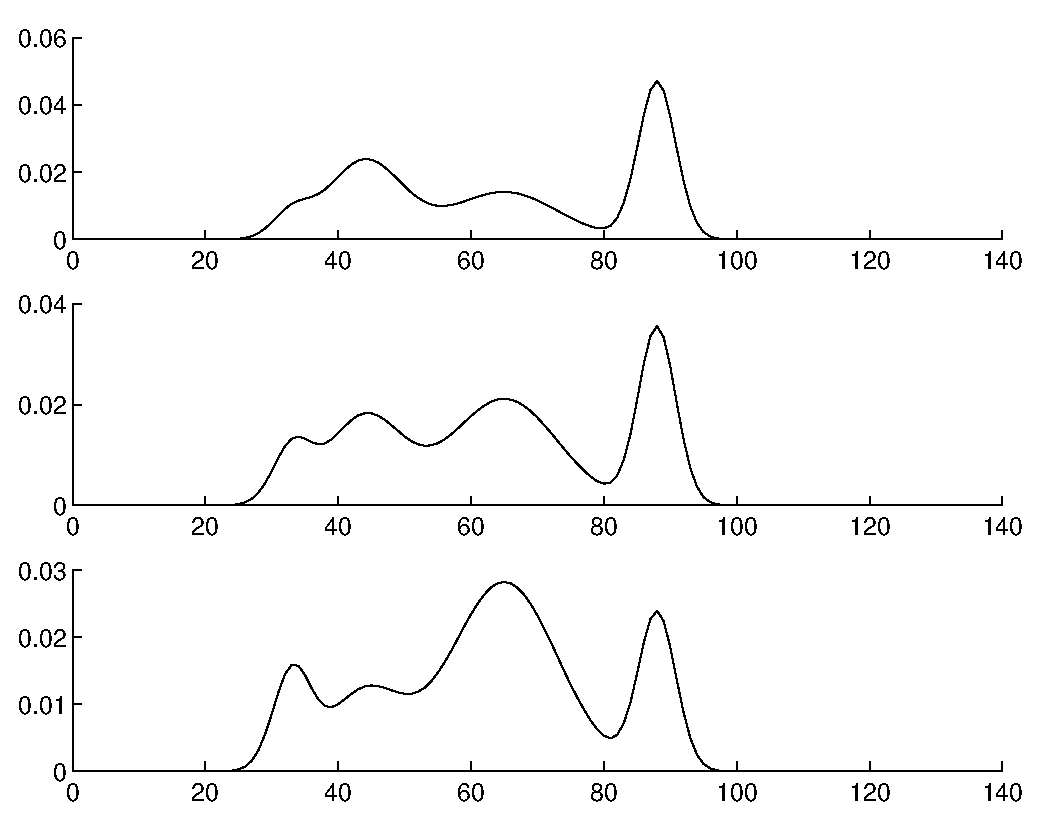
\includegraphics[width=0.5\textwidth]{figures/melang.eps}
\end{figure}

\end{frame}


\begin{frame}
\frametitle{Données sous forme matricielle}

$P$ échantillons, $N$ variables explicatives : matrice $P\times N$

\begin{figure}
\begin{figure}
\captionsetup{labelformat=empty}
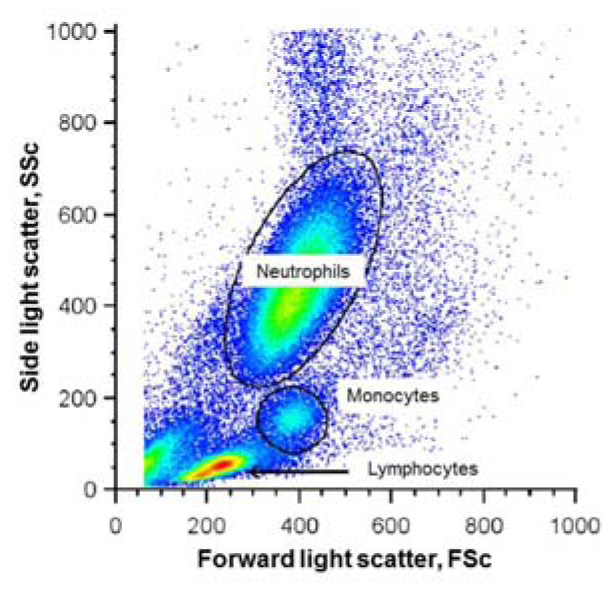
\includegraphics[width=0.4\textwidth]{figures/cyto}
\caption{\url{https://blog_fr.interchim.com/cytometrie-flux-analyse-cellulaire/}}
\end{figure}
\end{figure}


\end{frame}

\begin{frame}
\frametitle{Données sous forme matricielle}

Images (en niveaux de gris)

\begin{figure}
\captionsetup{labelformat=empty}
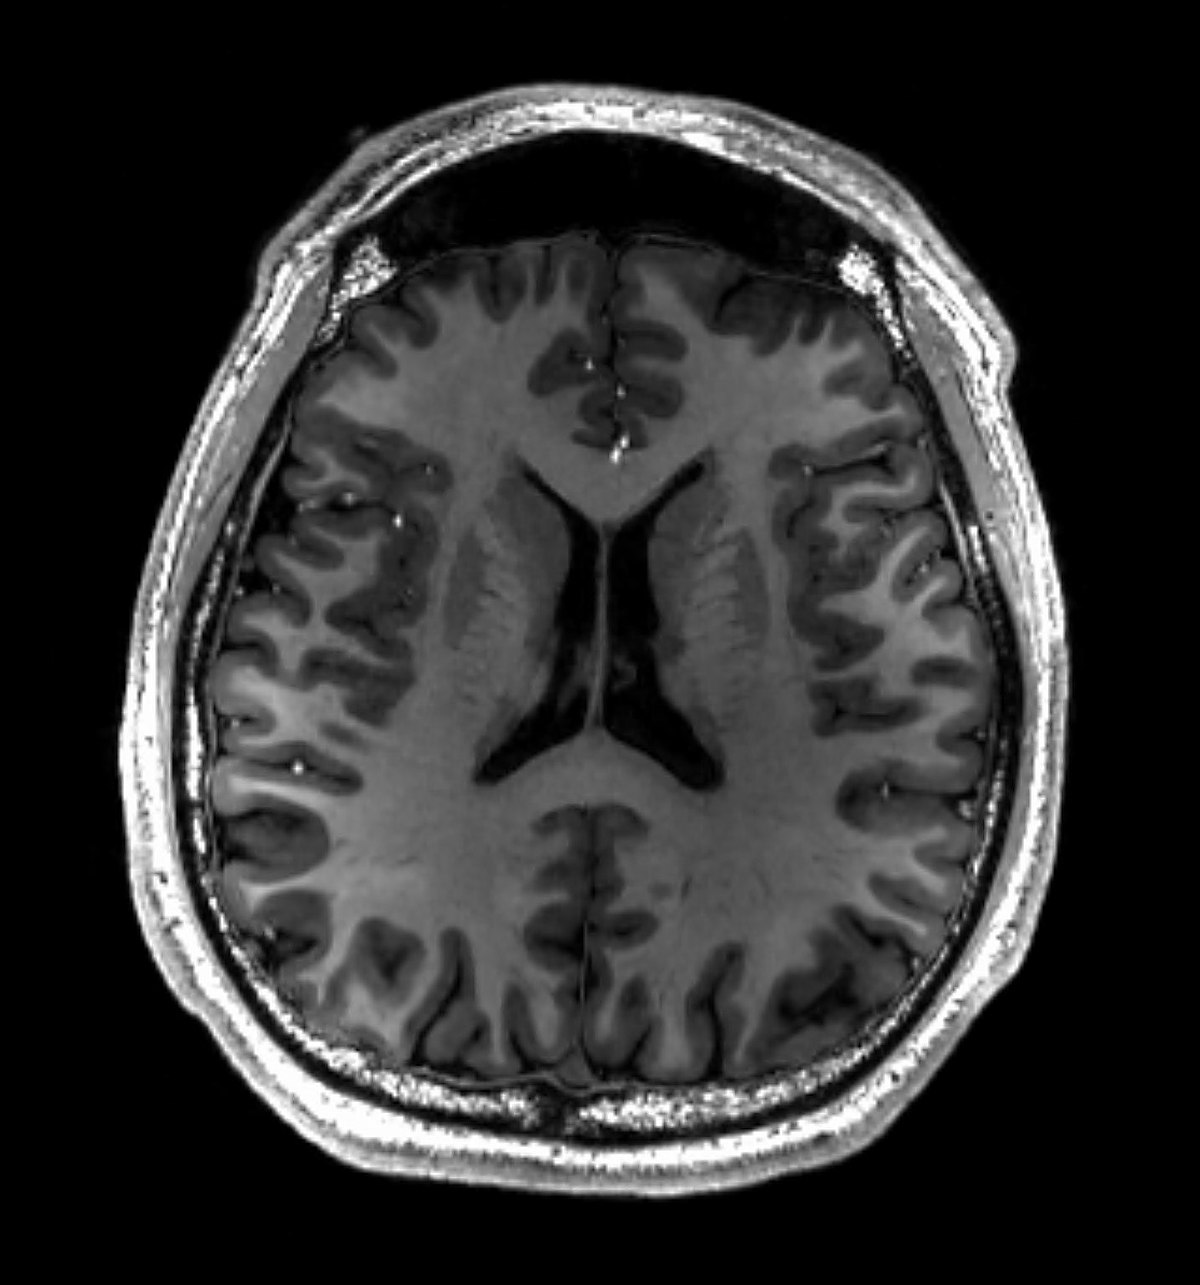
\includegraphics[width=0.4\textwidth]{figures/mri}
\caption{(wikipedia)}
\end{figure}
\end{frame}


\begin{frame}
\frametitle{Matrices à partir de données}

Statistiques des données: matrice de covariance, histogrammes

\begin{figure}
\captionsetup{labelformat=empty}
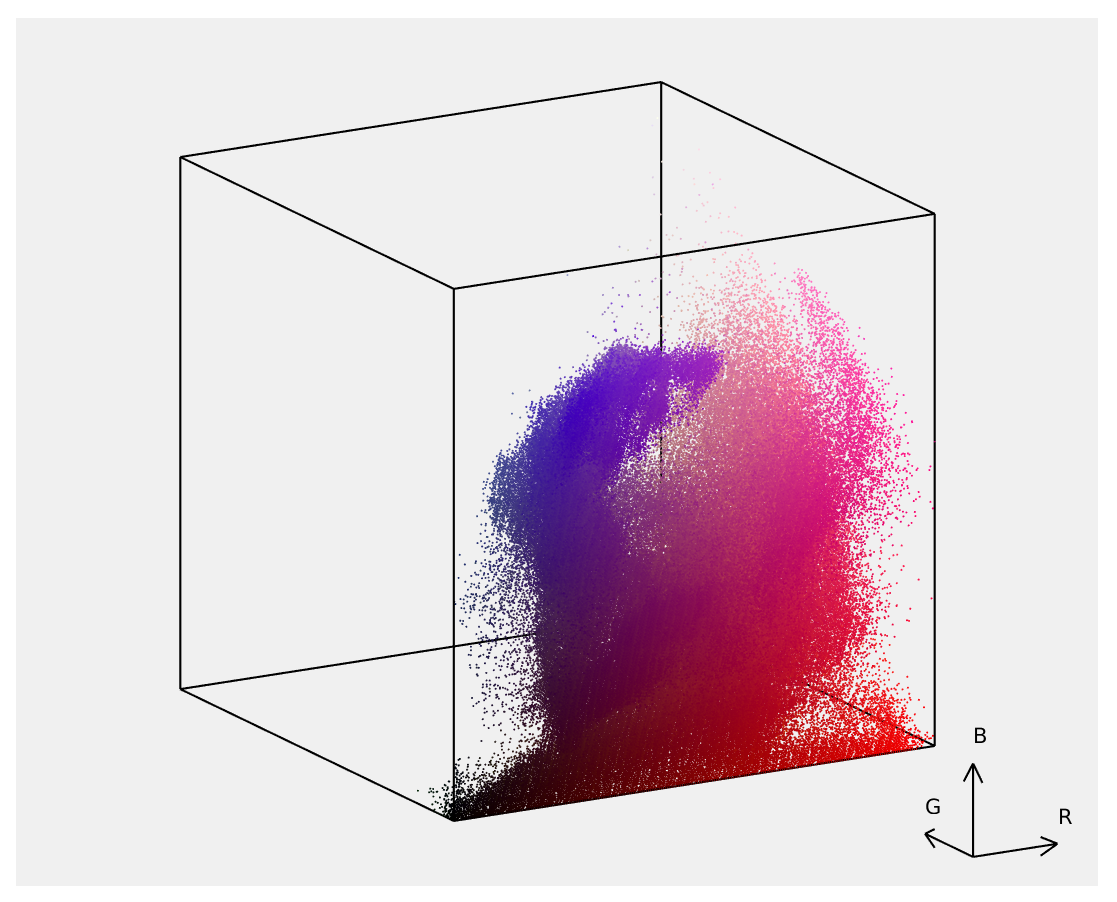
\includegraphics[width=0.5\textwidth]{figures/colorcloud}
\end{figure}

\end{frame}


\begin{frame}
\frametitle{Matrices à partir de données}

Matrices d'adjacence, Laplaciens (données sur graphe)

\begin{figure}
\captionsetup{labelformat=empty}
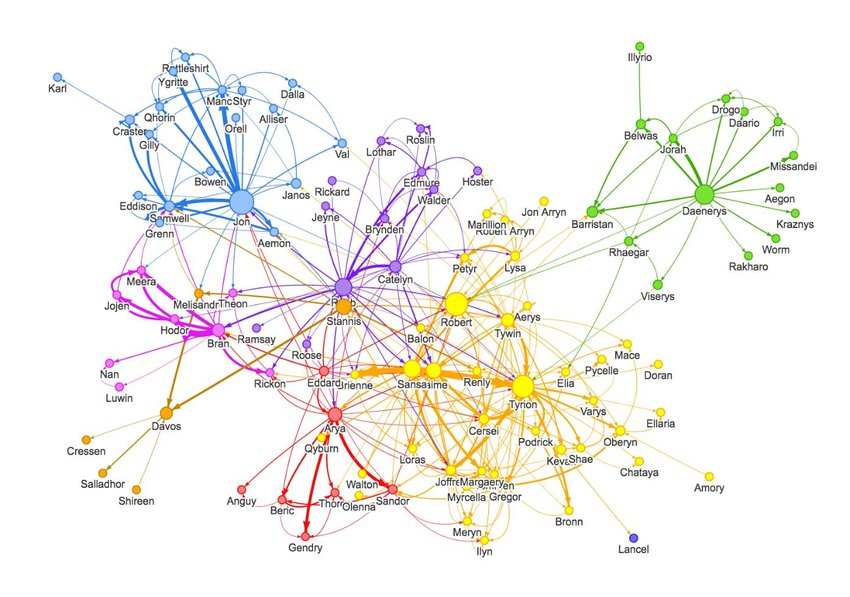
\includegraphics[width=0.6\textwidth]{figures/graph}
\caption{\tiny{\url{https://machinelearningknowledge.ai/graph-neural-networks-gnn-explained-for-beginners/}}}
\end{figure}

\end{frame}



%\begin{frame}
%\frametitle{Matrices: notations}
%\begin{itemize}[label=-]
%\item  \alert{Matrice}: $\mathbf{X} \in \mathbb{R}^{m \times n},\quad
%\raisebox{-0.25\height}{\begin{tikzpicture}[scale=0.8]
%\draw(0,0.5) node (A) {$\mathbf{X}$};
%\draw(-1.1,0.5) node (eq) {\footnotesize ${m}$};
%\draw(0,1.4) node (eq) {\footnotesize ${n}$};
%\draw(-0.7,0) rectangle (0.7,1);\end{tikzpicture}}$
%\item \alert{éléments} de la matrice: $ \mathbf{X}_{ij}$ 
%\item \alert{lignes}: $\mathbf{X}_{i,:} = [(\mathbf{X})_{i1}, (\mathbf{X})_{i2}, \ldots, (\mathbf{X})_{iJ} ]$
%\item \alert{colonnes}: $\mathbf{X}_{:,j} = [(\mathbf{X})_{1j}, (\mathbf{X})_{2j}, \ldots, (\mathbf{X})_{Ij} ]$
%\item \alert{sous-matrice}: $\mathbf{X}_{i_1:i_2,j_1:j_2} = [\mathbf{X}_{ij}]_{i=i_1,j=j_1}^{i_2,j_2}$
%
%\item \alert{transposition}, \alert{inversion}: $(\cdot)^T, (\cdot)^{-1}$
%
%\item \alert{matrice diagonale}:
%\[
%\text{diag}\{a_1, \dots,  a_p \} = 
%\begin{bmatrix}
%a_1 & 				& \\
%		& \ddots 	& \\
%		& 				& a_p
%\end{bmatrix}
%\]
%
%\end{itemize}
%\vfill
%\begin{itemize}
%	\item Dans MATLAB: {\tt X(i,j), \quad X(i,:), \quad X(:,j)}
%\end{itemize}
%
%\end{frame}



\begin{frame}
\frametitle{Décompositions/ factorisations  matricielles}

\begin{tcolorbox}[colback=blue!15,width=1.01\textwidth]
\[\tag{Décomposition}
\mathbf{X} \in \mathbb{R}^{m \times n}, \quad \mathbf{X} = \mathbf{a}_{1} \mathbf{s}_{1}^T + \cdots + \mathbf{a}_{p} \mathbf{s}_{p}^T = \sum_{k=1}^p  \mathbf{a}_{k} \mathbf{s}_{k}^T 
\]
\end{tcolorbox}

\begin{tcolorbox}[colback=green!15,width=1.01\textwidth]
Notation :
$\mathbf{A}=[\mathbf{a}_1 | \dots | \mathbf{a}_p ] ; \hspace{.5cm} \mathbf{S}=[\mathbf{s}_1 | \dots | \mathbf{s}_p ] $ \;  $\leadsto$ \; $\mathbf{X} = \mathbf{A} \,  \mathbf{S}^T $
\[\tag{Factorisation}
\raisebox{-0.35\height}{\begin{tikzpicture}[scale=0.8]
\draw(0,0.5) node (A) {$\mathbf{X}$};
\draw(-1.1,0.5) node (eq) {\footnotesize ${m}$};
\draw(0,1.4) node (eq) {\footnotesize ${n}$};
\draw(-0.7,0) rectangle (0.7,1);
\draw(1.1,0.5) node (eq) {${=}$};
\draw(1.6,0) -- (1.6,1);
\draw(1.6,0.5) node[fill=green!15] (a1) {{ $\bfa_1$}};
\draw(1.7,1) -- (3.08,1);
\draw(2.35,1) node[fill=green!15] (b1) {{\small $\bfs_1^{\T}\!\!$}};
\draw(3.5,0.5) node () {{\small $+\; \cdots\;+$}};
\draw(4.6,0) -- (4.6,1);
\draw(4.6,0.5) node[fill=green!15] (a1) {{ $\bfa_p$}};
\draw(4.7,1) -- (6.08,1);
\draw(5.35,1) node[fill=green!15] (b1) {{\small $\bfs_p^{T}\!\!$}};
\end{tikzpicture}}
\raisebox{-0.35\height}{\begin{tikzpicture}[scale=0.8]
%\draw(0,0.5) node (A) {$\mathbf{X}$};
%\draw(-1.1,0.5) node (eq) {\footnotesize ${m}$};
%\draw(0,1.4) node (eq) {\footnotesize ${n}$};
%\draw(-0.8,0) rectangle (0.8,1.2);
\draw(1.2,0.5) node (eq) {$=$};

\draw(1.7,0.5) node (eq) {\footnotesize ${m}$};

\draw(2,0) rectangle (2.6,1.2); %node {A};
\draw(2.3,0.6) node (A) {$\mathbf{A}$};

\draw(2.3,1.4) node (eq) {\footnotesize ${p}$};
%\draw(5,0.5) node (eq) {\footnotesize$\quad+\,\cdots\,+\quad$};
\draw(3.5,1.4) node (eq) {\footnotesize ${n}$};

\draw(3,0.65) rectangle (4.2,1.2); %node {A};
\draw(2.8,0.95) node (eq) {\footnotesize ${p}$};
\draw(3.6,0.95) node (A) {$\mathbf{S}^{T}$};
\end{tikzpicture}}
\]
\end{tcolorbox}

\vfill

%\begin{tcolorbox}[width=1.01\textwidth]
\textbf{Rang d'une matrice} : 
\begin{itemize}
\item[$(i)$] nombre de colonnes (ou lignes) indépendantes
\item[$(ii)$] nombre minimal de matrices de rang 1 permettant de représenter $\mathbf{X}$
\item[$(iii)$] taille minimale de la factorisation $\mathbf{A} \mathbf{B}^T $
\end{itemize}
%\end{tcolorbox}
 
On a toujours $\rank X \leq \min(m,n)$
%No
%$\Rightarrow$ \textbf{Approximation de rang faible}\\[2ex]
%\textbf{Indéterminations} : ordre, échelle, rotation
%\begin{equation*} 
%\mathbf{A} \mathbf{B}^T = (\mathbf{A} \mathbf{T}) ( \mathbf{T}^{-1}\mathbf{B}^T)  
%= \tilde{\mathbf{A}} \tilde{\mathbf{B}}^T 
%\end{equation*}
\end{frame}



\begin{frame}
\frametitle{Matrices de faible rang}

\begin{figure}
\captionsetup[subfigure]{labelformat=empty}
	\subfloat[rang = \only<2->{1}]{
\includegraphics[width=0.3\textwidth]{figures/flag-austria}}
	\;\;\vrule\;
	\subfloat[rang = \only<3->{2}]{
\includegraphics[width=0.3\textwidth]{figures/flag-denmark}}
	\;\;\vrule\;
	\subfloat[rang = \only<3->{3}]{
\includegraphics[width=0.3\textwidth]{figures/flag-greece}}
\end{figure}
\end{frame}



\begin{frame}
\frametitle{Faible rang = structure}

\begin{figure}
	\captionsetup[subfigure]{labelformat=empty}
	\subfloat[rang $\simeq \frac{m}{2}$ (symmetry)]{
\includegraphics[height=0.2\textwidth]{figures/flag-scotland}}
	\hspace{2cm}
	\subfloat[rang $\simeq \min(n,m)$ (aléatoire)]{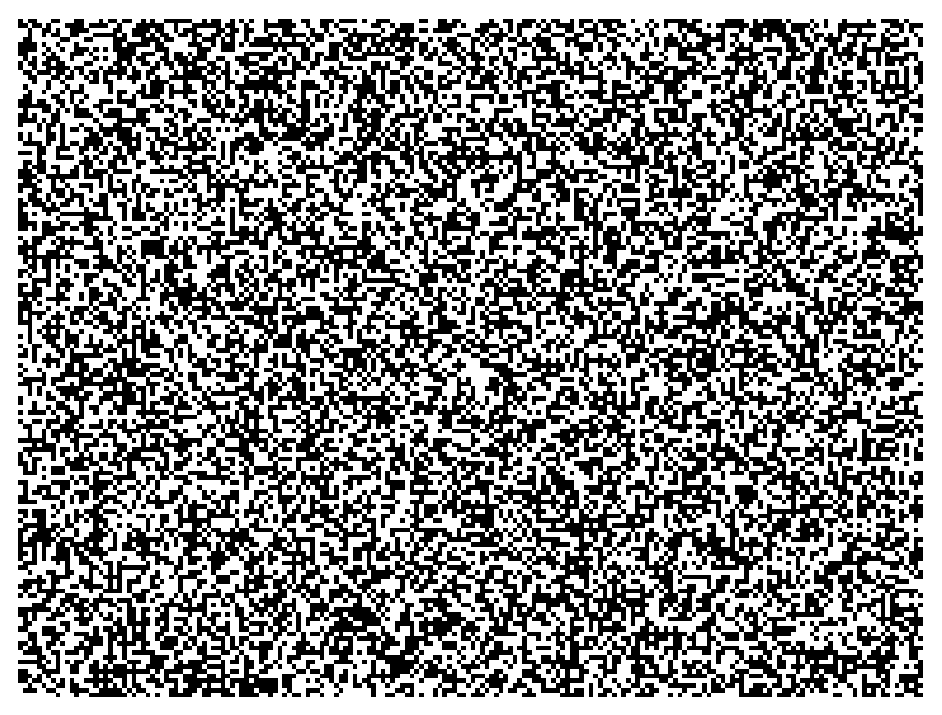
\includegraphics[height=0.2\textwidth]{figures/qrcode}}
\end{figure}

\pause

\begin{tcolorbox}
Beaucoup de matrices intéressantes en pratique sont (bien approximées par) des matrices de faible rang
\end{tcolorbox}

\end{frame}



\begin{frame}
\frametitle{Unicité?}

\begin{itemize}[label=\tiny$\blacksquare$]
	\item Les décompositions/factorisations de matrices ne sont \alert{pas uniques!}
	
	Par exemple, avec $T$ orthogonale, \ie\; $T^{-1} = T^\top$, on a toujours \[X = AS^\top = A T (ST)^\top\]
	
	$\leadsto$ la factorisation est aveugle aux \alert{permutations} de lignes/colonnes, \alert{agrandissement/rétrécissement}, \alert{rotations}, etc...
	
	\vfill
	
	\item Ajout de  \alert{\textbf{contraintes}} (orthogonalité, non-négativité, indépendance, ...) pour retrouver l'unicité
 
 $\leadsto$ décompositions particulières : SVD,  NMF, ICA, ...
 
	\vfill
 
	\item Dans ce cours, nous ne parlerons que de \alert{décomposition en valeurs singulières} (aka SVD)
\end{itemize}


\end{frame}


\section[SVD]{Décomposition en valeurs singulières (SVD)}


\begin{frame}[noframenumbering,plain]{Plan}
\tableofcontents[currentsection]
\end{frame}


\begin{frame}
\frametitle{Décomposition en valeurs singulières (SVD)}
		 \begin{center}
		
\includegraphics[width=6cm]{figures/keep-calm-and-be-orthogonal.eps}
	\end{center}
\end{frame}



%%%%%%%%%%%%%%%%%%%%%%%%%%%%%%%%%%%
\begin{frame}
\frametitle{Formulation}


\begin{theo} Soit $X \in \RR^{m\times n}$ de rang $r$. Il existe $\mathbf{U} \in \RR^{m\times m}$, $\mathbf{V} \in \RR^{n\times n}$ \alert{orthogonales}, et $\bm{\Sigma} \in \RR^{m\times n}$ \alert{diagonale} telles que
$$
	\mathbf{X} = \mathbf{U} \bm{\Sigma} \mathbf{V}^\top \quad\text{et}\quad \bm{\Sigma} = \begin{bmatrix} \diag(\sigma_1,\ldots,\sigma_r) & \large\bm{0} \\ \large\bm{0} & \large\bm{0} \end{bmatrix}
$$
avec $\sigma_1 \geq \sigma_2 \geq \ldots \geq \sigma_r > \sigma_{r+1} = \ldots = \sigma_p = 0$, et $p=\min(m,n)$.
\end{theo}

%\\[2ex] 


$\mathbf{U} = [\mathbf{u}_1 | \dots | \mathbf{u}_m ]$ : $(m \times m)$  matrice orthogonale (vecteurs singuliers gauches)\\[1ex]

$\mathbf{V} = [\mathbf{v}_1 | \dots | \mathbf{v}_n ]$ : $(n\times n)$ matrice orthogonale (vecteurs singuliers droits)\\[1ex]

 $\bm{\Sigma} = \text{diag}\{\sigma_1, \dots,  \sigma_p \}$ :  $(m \times n)$   matrice diagonale (valeurs singulières)\\[2ex] 
 
On a de manière équivalente la \alert{décomposition}
$$\tcbhighmath{
\mathbf{X} = \sum_{i=1}^p \sigma_i \, \mathbf{u}_i \,  \mathbf{v}_i^T}
$$

rang de $\mathbf{X}$ = nombre de valeurs singulières non-nulles

\end{frame}


\begin{frame}
\frametitle{Preuve}
\end{frame}

\begin{frame}
\frametitle{Preuve}
\end{frame}



\begin{frame}
\frametitle{Formes réduites}

\begin{itemize}[label=\tiny$\blacksquare$]
	\item par défaut (rappel: $p = \min(m,n)$)
		\[
\raisebox{-0.35\height}{\begin{tikzpicture}[scale=1]
\draw(-3,0.7) node (A) {$\mathbf{X}$};
\draw(-4.2,0.7) node (eq) {\footnotesize ${m}$};
\draw(-3,1.65) node (eq) {\footnotesize ${n}$};
\draw(-4.0,0) rectangle (-2.1,1.5);
\draw(-1.7,0.7) node (eq) {${=}$};


\draw(-1,0) rectangle (0.5,1.5);
\draw(-1.2,0.7) node (eq) {\footnotesize ${m}$};
\draw(-0.2,1.65) node (eq) {\footnotesize ${m}$};
\draw(-0.2,0.7) node (U) {$\mathbf{U}$};

\draw(0.9,0) rectangle (2.8,1.5);
%\draw(0.7,1) node (S) {$\mathbf{\Sigma}$};
\draw(1.12,1.36) node (S) {$\mathbf{\sigma_1}$};
\draw(1.31,1.1) node (S) {$\mathbf{\cdot}$};
\draw(1.65,0.73) node (S) {$\mathbf{\cdot}$};
\draw(1.99,0.41) node (S) {$\mathbf{\cdot}$};
\draw(2.18,0.15) node (S) {$\mathbf{\sigma_p}$};
\draw(0.7,0.7) node (eq) {\footnotesize ${m}$};
\draw(1.9,1.65) node (eq) {\footnotesize ${n}$};


\draw(3.2,-0.3) rectangle (5,1.5);
\draw(3.05,0.65) node (eq) {\footnotesize ${n}$};
\draw(4.1,1.65) node (eq) {\footnotesize ${n}$};
\draw(4.2,0.6) node (A) {$\mathbf{V}^{T}$};

\draw(5.3,0.7) node (eq) {${=}$};
\draw(6.3,0.7) node (eq) {$\displaystyle \sum_{i=1}^p \sigma_i \mathbf{u}_i\mathbf{v}_i^\top$};


\end{tikzpicture}}
\]
	
	
	\item "economy size"
			\[
\raisebox{-0.35\height}{\begin{tikzpicture}[scale=1]
\draw(-3,0.7) node (A) {$\mathbf{X}$};
\draw(-4.2,0.7) node (eq) {\footnotesize ${m}$};
\draw(-3,1.65) node (eq) {\footnotesize ${n}$};
\draw(-4.0,0) rectangle (-2.1,1.5);
\draw(-1.7,0.7) node (eq) {${=}$};


\draw(-1,0) rectangle (0.5,1.5);
\draw(-1.2,0.7) node (eq) {\footnotesize ${m}$};
\draw(-0.2,1.65) node (eq) {\footnotesize ${p}$};
\draw(-0.2,0.7) node (U) {$\mathbf{U}$};

\draw(0.9,0) rectangle (2.4,1.5);
%\draw(0.7,1) node (S) {$\mathbf{\Sigma}$};
\draw(1.12,1.36) node (S) {$\mathbf{\sigma_1}$};
\draw(1.31,1.1) node (S) {$\mathbf{\cdot}$};
\draw(1.65,0.73) node (S) {$\mathbf{\cdot}$};
\draw(1.99,0.41) node (S) {$\mathbf{\cdot}$};
\draw(2.18,0.15) node (S) {$\mathbf{\sigma_p}$};
\draw(0.7,0.7) node (eq) {\footnotesize ${p}$};
\draw(1.7,1.65) node (eq) {\footnotesize ${p}$};


\draw(2.8,0) rectangle (4.7,1.5);
\draw(2.65,0.7) node (eq) {\footnotesize ${p}$};
\draw(3.8,1.65) node (eq) {\footnotesize ${n}$};
\draw(3.9,0.7) node (A) {$\mathbf{V}^{T}$};

\draw(5.3,0.7) node (eq) {${=}$};
\draw(6.3,0.7) node (eq) {$\displaystyle \sum_{i=1}^p \sigma_i \mathbf{u}_i\mathbf{v}_i^\top$};


\end{tikzpicture}}
\]


	\item forme réduite (si $\rank X = r < p$)
	\[
\raisebox{-0.35\height}{\begin{tikzpicture}[scale=1]
\draw(-3,0.7) node (A) {$\mathbf{X}$};
\draw(-4.2,0.7) node (eq) {\footnotesize ${m}$};
\draw(-3,1.65) node (eq) {\footnotesize ${n}$};
\draw(-4.0,0) rectangle (-2.1,1.5);
\draw(-1.7,0.7) node (eq) {${=}$};


\draw(-1,0) rectangle (-0.2,1.5);
\draw(-1.2,0.7) node (eq) {\footnotesize ${m}$};
\draw(-0.6,1.65) node (eq) {\footnotesize ${r}$};
\draw(-0.6,0.7) node (U) {$\mathbf{U}$};

\draw(0.2,0.5) rectangle (1.2,1.5);
%\draw(0.7,1) node (S) {$\mathbf{\Sigma}$};
\draw(0.42,1.36) node (S) {$\mathbf{\sigma_1}$};
\draw(0.7,1.13) node (S) {$\mathbf{\ddots}$};
\draw(0.98,0.65) node (S) {$\mathbf{\sigma_r}$};
\draw(0,1) node (eq) {\footnotesize ${r}$};
\draw(0.7,1.65) node (eq) {\footnotesize ${r}$};


\draw(1.65,0.5) rectangle (3.5,1.5);
\draw(1.45,0.95) node (eq) {\footnotesize ${r}$};
\draw(2.6,1.65) node (eq) {\footnotesize ${n}$};
\draw(2.6,1) node (A) {$\mathbf{V}^{T}$};

\draw(4,0.7) node (eq) {${=}$};
\draw(5,0.7) node (eq) {$\displaystyle \sum_{i=1}^r \sigma_i \mathbf{u}_i\mathbf{v}_i^\top$};



\end{tikzpicture}}
\]
\end{itemize}

\end{frame}


\begin{frame}
\frametitle{Image et noyau}


\vfill
$$
	\begin{aligned}
		&\mathrm{Ker}\; \mathbf{X} = \mathrm{Vect}(v_{r+1},\ldots,v_n)\\
		&\mathrm{Im}\; \mathbf{X} = \mathrm{Vect}(u_1,\ldots,u_r)\\
		&\mathrm{Ker}\; \mathbf{X}^\top = \mathrm{Vect}(u_{r+1},\ldots,u_m)\\
		&\mathrm{Im}\; \mathbf{X}^\top = \mathrm{Vect}(v_1,\ldots,v_r)
	\end{aligned}
$$


\end{frame}



\begin{frame}
\frametitle{SVD et rang}

\begin{figure}
	\captionsetup[subfigure]{labelformat=empty}
	\subfloat[rang=2]{
\includegraphics[width=0.3\textwidth]{figures/flag-denmark}}
	\;
	\subfloat[rang=3]{
\includegraphics[width=0.3\textwidth]{figures/flag-greece}}
	\;
	\subfloat[rang=?]{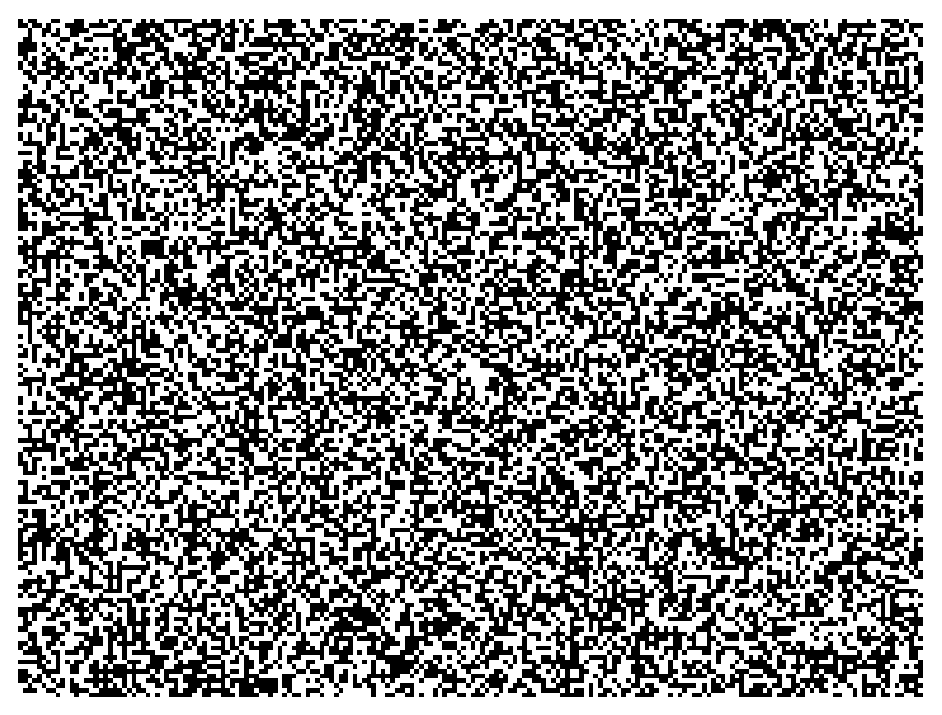
\includegraphics[height=0.225\textwidth]{figures/qrcode}}
	\\
	\subfloat[rang=2]{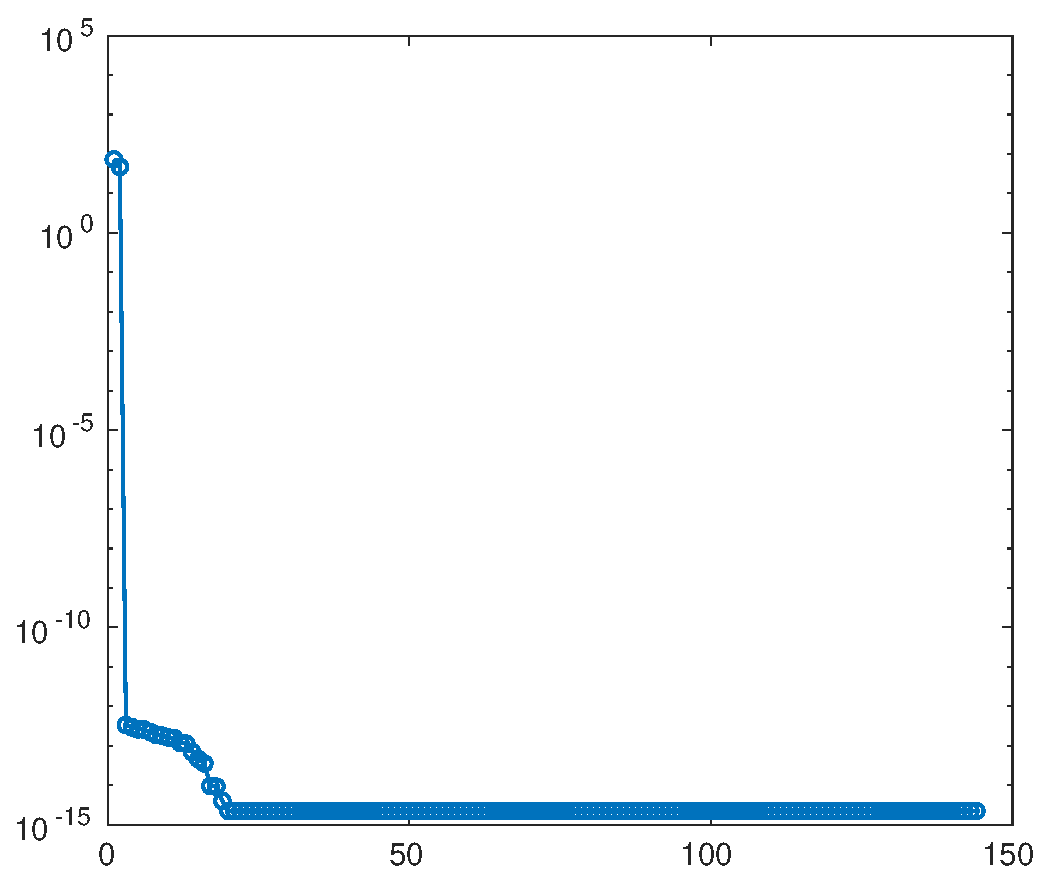
\includegraphics[width=0.3\textwidth]{figures/svd-denmark}}
	\;
	\subfloat[rang=3]{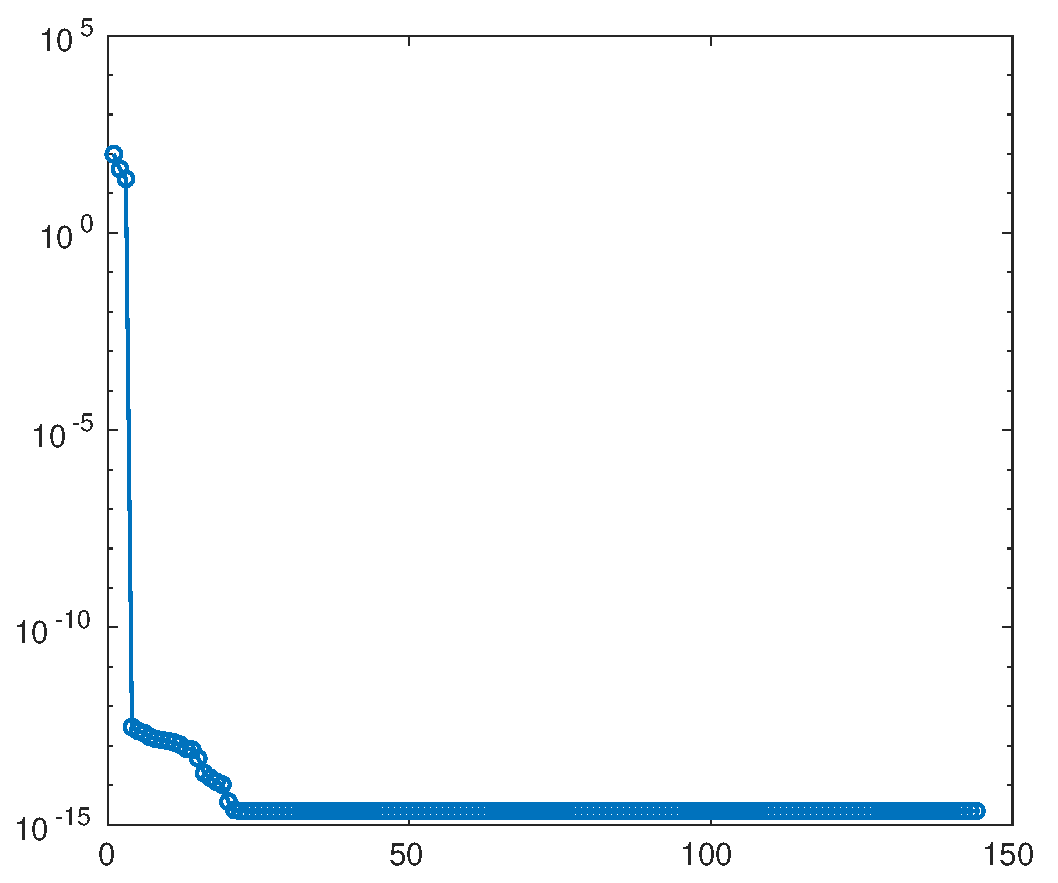
\includegraphics[width=0.3\textwidth]{figures/svd-greece}}
	\;
	\subfloat[rang=?]{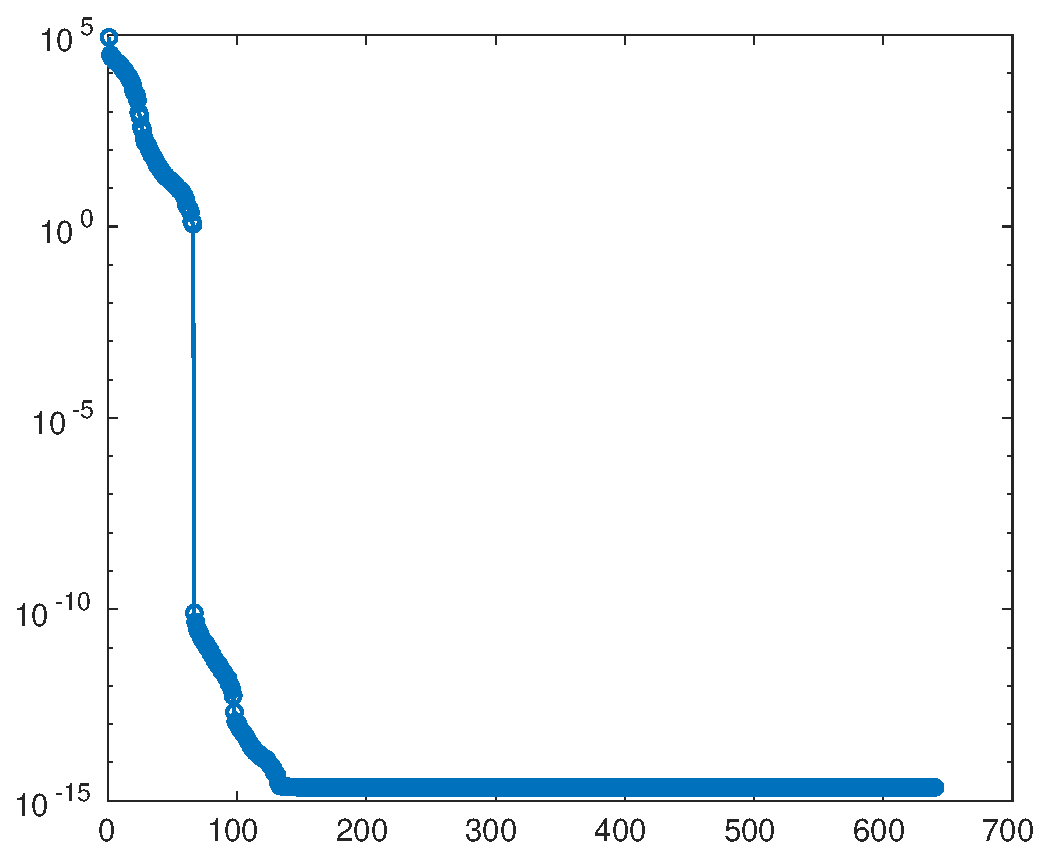
\includegraphics[width=0.3\textwidth]{figures/svd-qrcode}}
\end{figure}

\end{frame}





%%%%%%%%%%%%%%%%%%%%%%%%%%%%%%%%%%%
\begin{frame}
\frametitle{SVD et la décomposition en valeurs propres (EVD)}
	
$$\mathbf{X} \,  \mathbf{X}^T = \mathbf{U} \, \bm{\Sigma}^2 \, \mathbf{U}^T$$


$$\mathbf{X}^T  \mathbf{X} = \mathbf{V} \, \bm{\Sigma}^2 \, \mathbf{V}^T$$
\

\

\begin{itemize}[label=\tiny$\blacksquare$]
	\item  Les \alert{vecteurs singuliers gauches}  $\mathbf{U}$ sont les vecteurs propres de $\mathbf{X} \,  \mathbf{X}^T$.\\[3ex]
	
	\item  Les \alert{vecteurs singuliers droits} $\mathbf{V}$ sont les vecteurs propres de $\mathbf{X}^T  \mathbf{X}$.\\[3ex]
	
	\item Les \alert{valeurs singulières} (non-nulles) de $\mathbf{X}$ sont les racines carrées des valeurs propres (non-nulles) de $\mathbf{X}^T  \mathbf{X}$ ou $\mathbf{X} \,  \mathbf{X}^T$. En particulier, elles sont déterminées de manière \alert{unique}.\\[3ex]
\end{itemize}

\end{frame}	
%%%%%%%%%%%%%%%%%%%%%%%%%%%%%%%%%%%

%%%%%%%%%%%%%%%%%%%%%%%%%%%%%%%%%%%
\begin{frame}
	
	\frametitle{Approximation de rang faible}
	
	
	
	
	Soit $\mathbf{X} \in \RR^{m\times n}$ et soit $(\mathbf{U},\bm{\Sigma}, \mathbf{V})$ sa factorisation SVD. Pour $s \leq \min(m,n)$, la matrice
	$$
		\mathbf{X}_r \eqdef \sum_{i=1}^s \sigma_i u_i v_i^\top
	$$
	donne la meilleure approximation de rang faible d'une matrice au sens de la norme de Frobenius $\norm{ \mathbf{X} }_F = \Tr(X^\top X) = \sqrt{\sigma_1^2 +\dots +\sigma_p^2} .$
	 
	\begin{tcolorbox}	
	la solution du problème d'optimisation
	
	$$
	\min\left\lVert \mathbf{X} - \mathbf{X}_r \right\rVert_F \quad \text{s. c.} \quad \text{rang}( \mathbf{X}_r) \leq r, \quad r<p
	$$
	
	est donnée par : $
	\boxed{\mathbf{X}_r =  \sum_{i=1}^r \sigma_i \, \mathbf{u}_i \,  \mathbf{v}_i^T}$
	\end{tcolorbox}
	
	\vfill
	
	Forme matricielle: $\mathbf{X}_r = \mathbf{U}_{:,1:r} \bm{\Sigma}_{1:r,1:r} (\mathbf{V}_{:,1:r})^{T}$
	
	L'erreur de la meilleure approximation: $\lVert \mathbf{X} - \mathbf{X}_r \rVert_F = \sqrt{\begin{smallmatrix}\sigma_{r+1}^2 +\dots +\sigma_p^2\end{smallmatrix}}$
	
\end{frame}	





\section{Applications}
\begin{frame}[noframenumbering,plain]{Plan}
\tableofcontents[currentsection]
\end{frame}




%%%%%%%%%%%%%%%%%%%%%%%%%%%%%%%%%%%
\begin{frame}
	
	\frametitle{Applications de la SVD}
	
	\begin{itemize}[label=\tiny$\blacksquare$]
	\item Compression et débruitage (traitement d'image, sismique, ...). \\[3ex]
	
	\item Extraction des motifs et analyse des textures. \\[3ex]
	
	\item Analyse en composantes principales (statistique, systèmes de recommandations,...).\\[3ex]
	
	\item Résolution de systèmes d'équations linéaires (calcul de la pseudo-inverse).\\[3ex]
		
	\end{itemize}	
	
	\
	
	\begin{center}
		\large
		\textbf{Algorithmes pour la SVD}
	\end{center}
	

	
Méthodes pour la décomposition en valeurs propres, algorithmes {\em gloutons} (Gram-Schmidt, ...), factorizations QR, {\em etc.}

	
\end{frame}	
%%%%%%%%%%%%%%%%%%%%%%%%%%%%%%%%%%%



%%%%%%%%%%%%%%%%%%%%%%%%%%%%%%%%%%%
\begin{frame}
	\frametitle{Débruitage et compression d'image (1)}
	
	\begin{columns}
   		 \column{0.5\textwidth}
   		 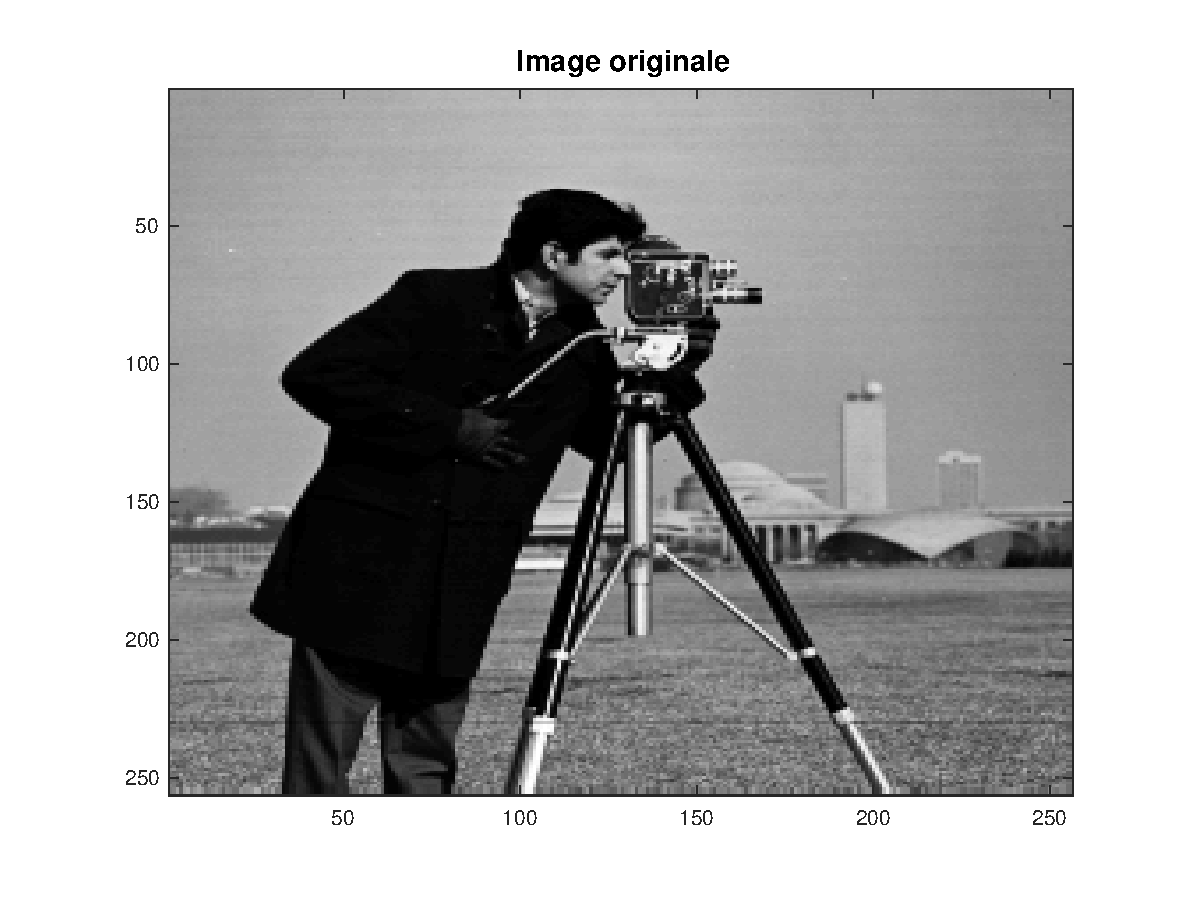
\includegraphics[scale=.3]{figures/cam_orig.eps}
 
    		\column{0.5\textwidth}
    		 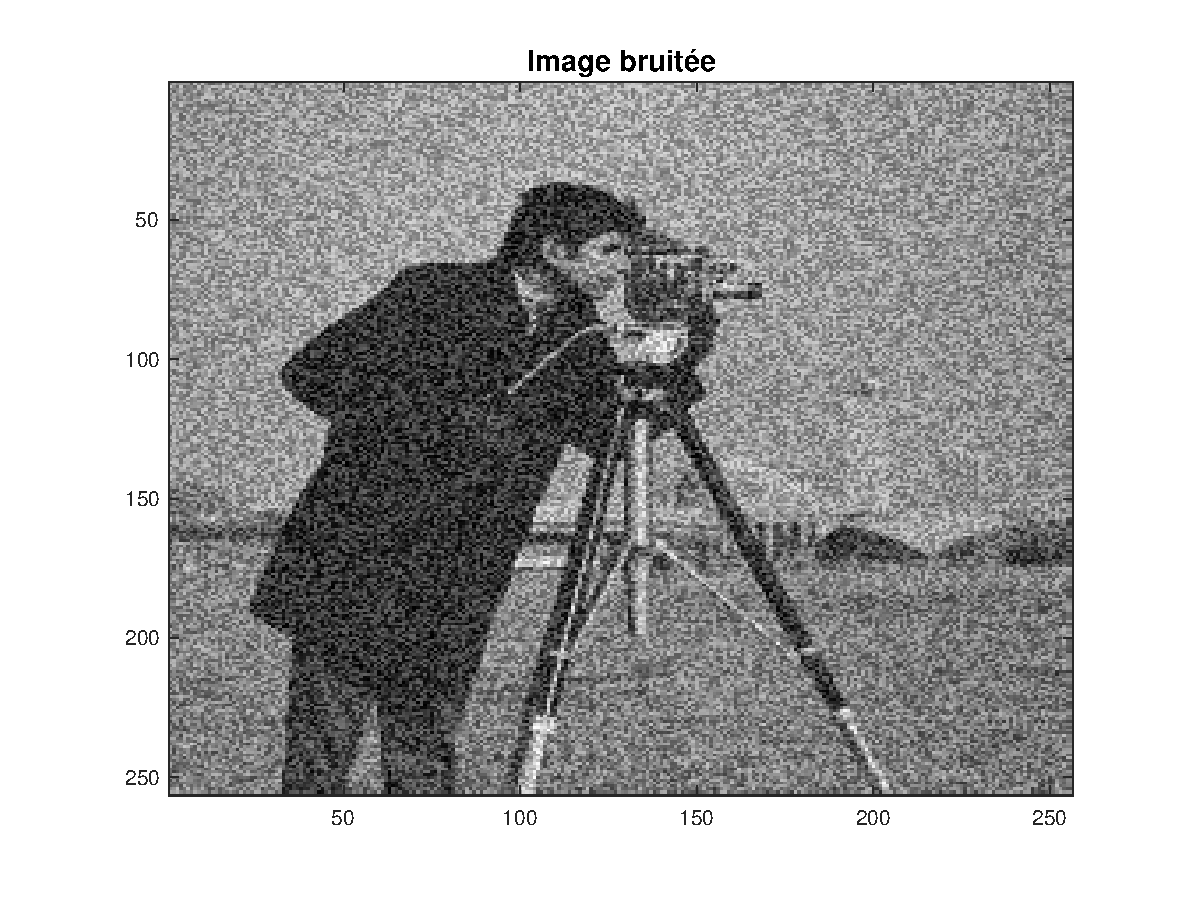
\includegraphics[scale=.3]{figures/cam_noise.eps}
   \end{columns}
   \centering
   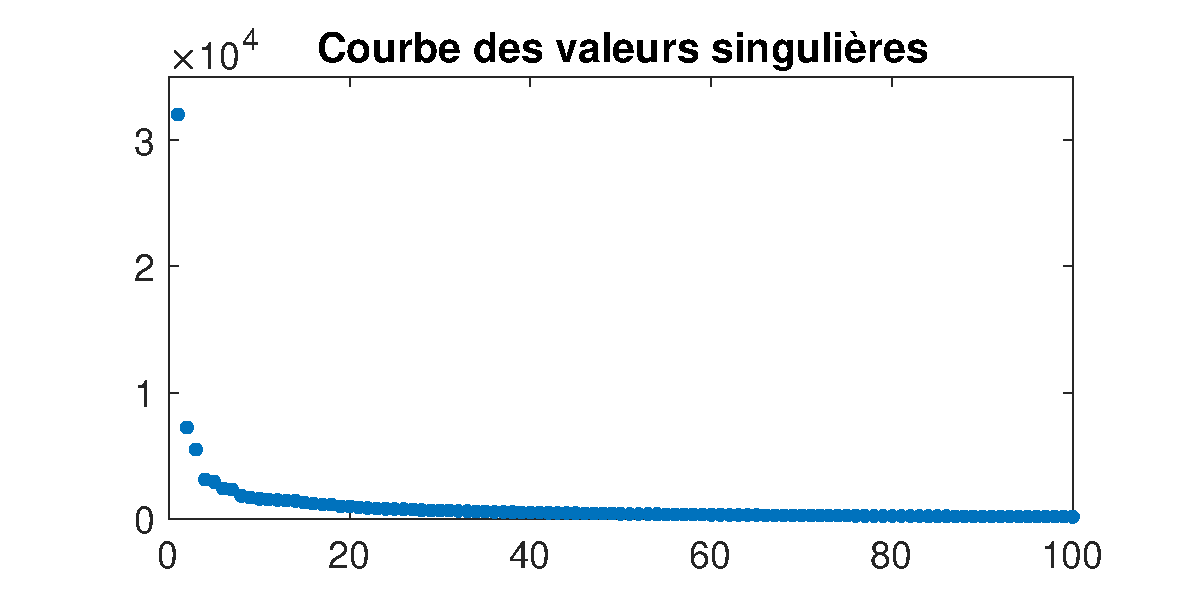
\includegraphics[scale=.3]{figures/sing_v.eps}
   
\end{frame}


%%%%%%%%%%%%%%%%%%%%%%%%%%%%%%%%%%%
%%%%%%%%%%%%%%%%%%%%%%%%%%%%%%%%%%%
\begin{frame}
	\frametitle{Débruitage et compression d'image (2)}
	\vspace{3pt}
	\begin{columns}
    		\column{0.5\textwidth}
		\centering
   		 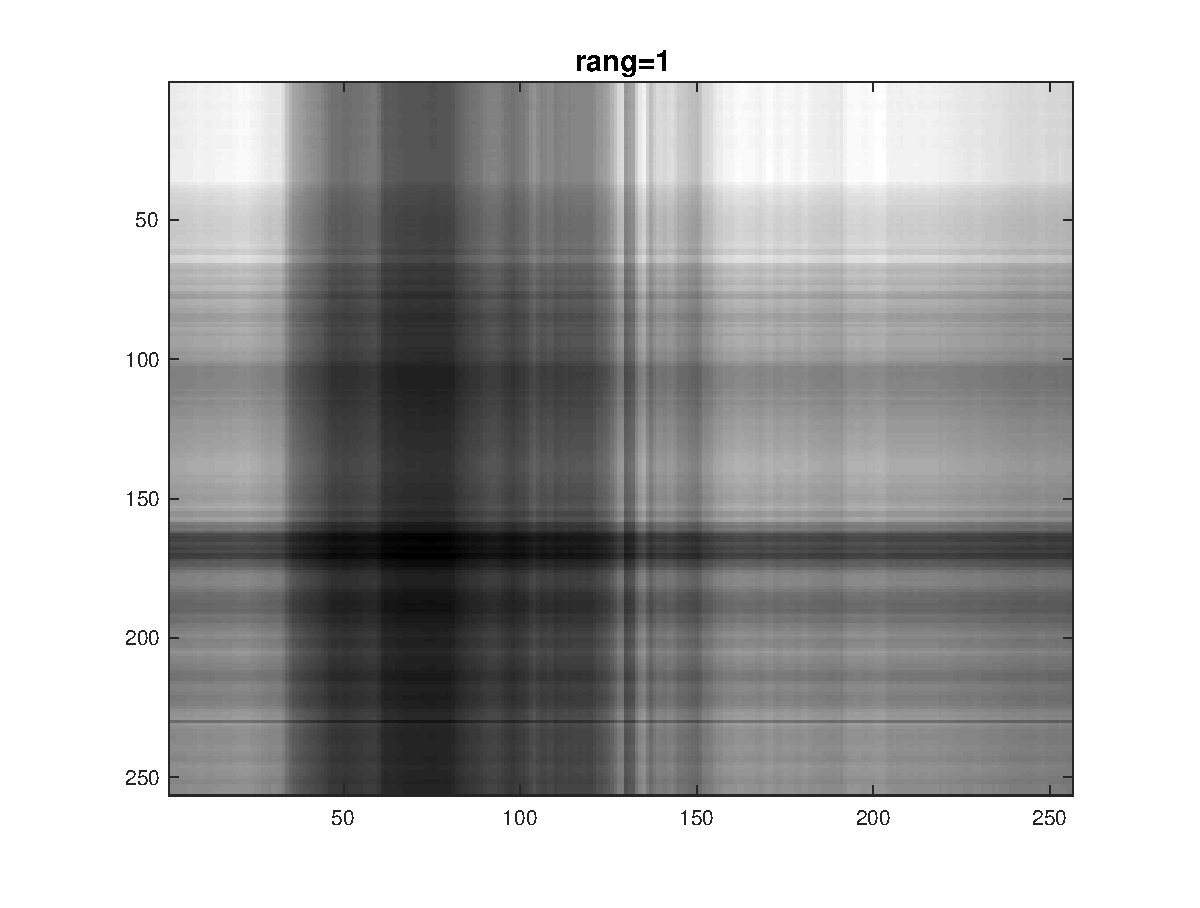
\includegraphics[scale=.29]{figures/cam_r1.eps}\\
		 
		  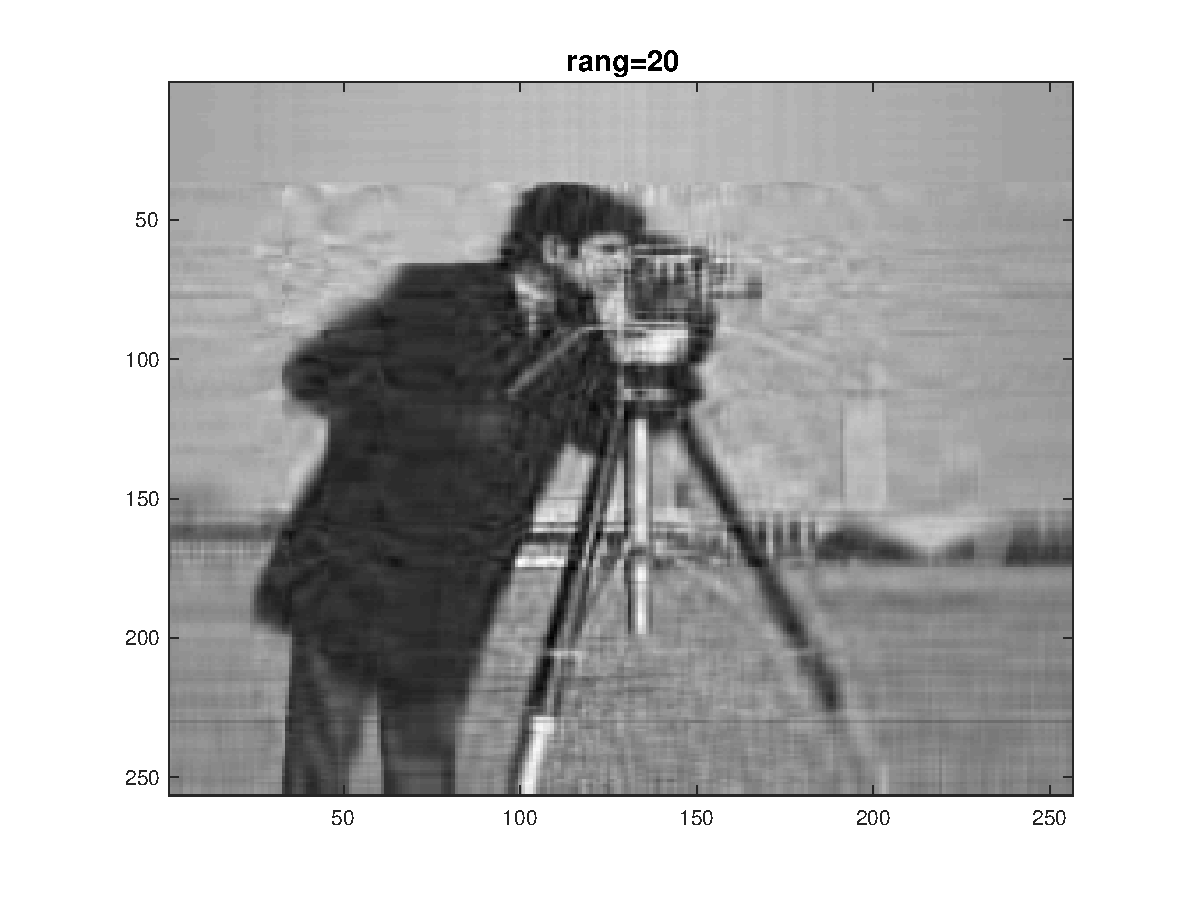
\includegraphics[scale=.29]{figures/cam_r20.eps}
 			
    		\column{0.5\textwidth}
		\centering
   		 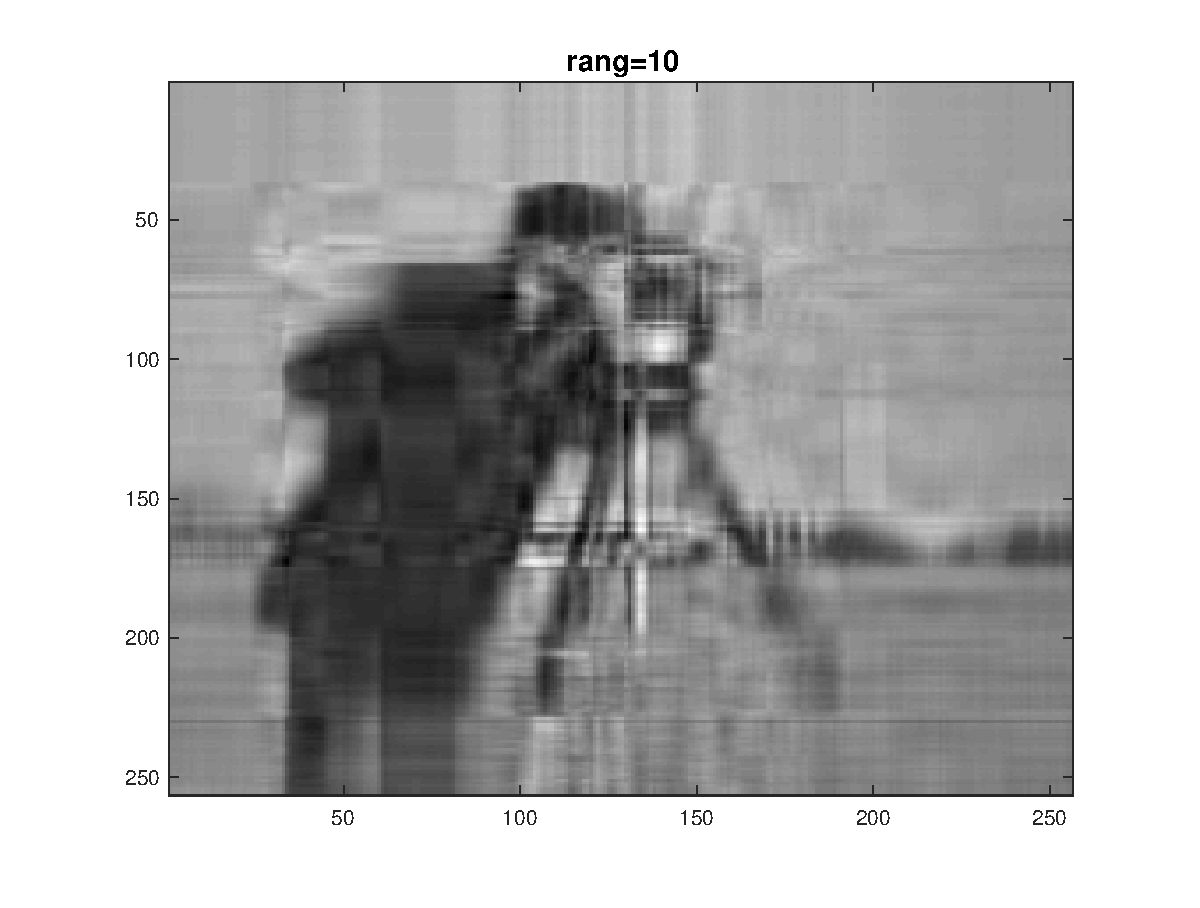
\includegraphics[scale=.29]{figures/cam_r10.eps}\\
		 
		  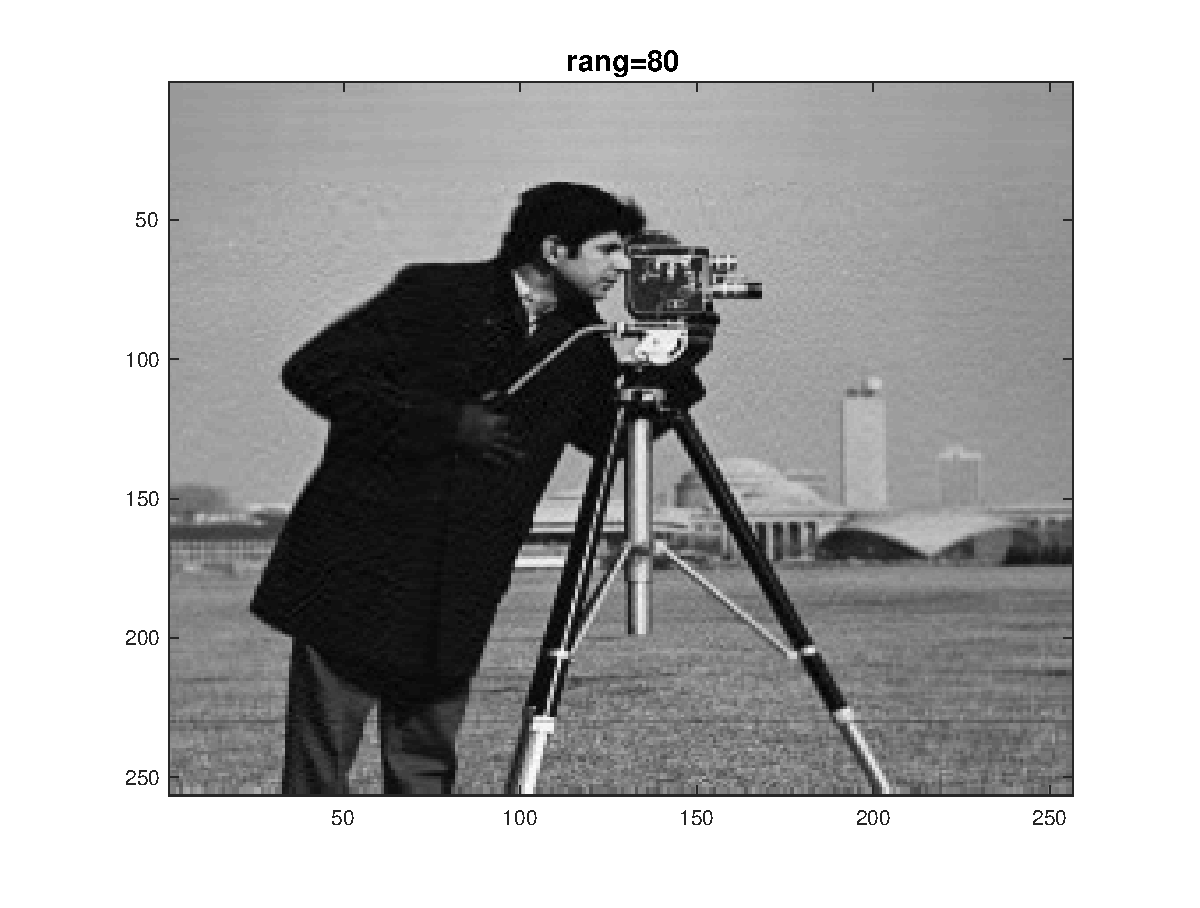
\includegraphics[scale=.29]{figures/cam_r80.eps}
   \end{columns}
\end{frame}


\begin{frame}
\frametitle{Moindres carrés}
Problème des moindres carrés:
$$
\min_{x\in\RR^n} \norm{Ax-y}_2^2
$$
étant donnés $A \in \RR^{m\times n}$ et $y\in\RR^m$.

$$\begin{aligned}
	\norm{Ax-u}_2^2 
		&= \norm{U\Sigma V^\top x -y}_2^2 = \norm{\Sigma V^\top x - U^\top y}_2^2\\
		&=\sum_{i=1}^r \abs{\sigma_i v_i^\top x - u_i^\top y}^2 + \sum_{i=r+1}^m \abs{u_i^\top y}^2
\end{aligned}$$
\vfill

Le minimum est atteint pour
$$\tcbhighmath{
	x_\star = \sum_{i=1}^r \frac{u_i^\top y}{\sigma_i}v_i + x_0 \eqdef x_+ + x_0}
$$
et $\norm{x_\star}^2 = \norm{x_+}^2 + \norm{x_0}^2 \geq \norm{x_+}^2$
\end{frame}

\begin{frame}
\frametitle{Pseudo-inverse}

$$
x_+ = \sum_{i=1}^r \frac{u_i^\top y}{\sigma_i}v_i = A^\dagger y \quad \text{où}\quad \tcbhighmath{A^\dagger \eqdef V \begin{bmatrix} \diag(\frac{1}{\sigma_1},\ldots,\frac{1}{\sigma_r}) & \large\bm{0} \\ \large\bm{0} & \large\bm{0} \end{bmatrix}U^\top}
$$
\vfill
	\begin{itemize}[label=\bullet]
	\item Si $A$ est injective, alors $A^\dagger y$ est l'unique solution du problème des moindres carrés
	
	\item Si $A$ n'est pas injective, alors $A^\dagger y$ est la solution du problème ayant la plus petite norme $\ell_2$
		\item $A^\dagger A A^\dagger = A^\dagger$
		\item $A A^\dagger A = A$
	\end{itemize}

\end{frame}

\begin{frame}
\frametitle{Analyse en composantes principales}

A partir de données $(x_1,\ldots,x_N) \in \RR^d$, on souhaite trouver une \alert{représentation optimale} $z \in \RR^{d'}$ avec $d' < d$ par \alert{projection orthogonale} sur un \alert{sous espace} bien choisi

Projection orthogonale $\iff$ base orthogonale $\mathbf{U} \in \RR^{d \times d'}$

$\mathbf{X} \in \RR^{d\times N}$ matrice de données $\iff$ ${\mathbf{Z}} = \mathbf{U}^\top \mathbf{X} \in \RR^{d'\times N}$ matrice des données projetées

\vfill

\begin{tcolorbox}
L'analyse en composante principale (ACP) est une \alert{factorisation matricielle} ($\mathbf{X} = \mathbf{W} \mathbf{Z}$) qui choisit $\mathbf{Z}$ avec les colonnes les plus \alert{décorrélées} possibles. Elle s'appuie logiquement sur la matrice de covariance des données.
\end{tcolorbox}

\end{frame}




\begin{frame}
\frametitle{Matrice de covariance}

La matrice de covariance d'un vecteur aléatoire $\mathbf{X}$ à valeurs dans $\RR^d$ est donnée par
$$
	\mathrm{Cov}(\mathbf{X}) = \mathbb{E}((\mathbf{X}-\mathbf{\mathbb{E}(X)})(\mathbf{X}-\mathbb{E}({\mathbf{X}}))^\top)
$$

A partir d'une matrice de données $\mathbf{X} = \begin{bmatrix} \mathbf{x}_1 & \ldots & \mathbf{x}_N \end{bmatrix}$, on peut calculer la matrice de covariance empirique:
$$\tcbhighmath{
\widehat{\mathbf{C}} = \frac{1}{N-1} \sum_{i=1}^N (\mathbf{x}_i - \mathbf{\overline{x}})(\mathbf{x}_i-\mathbf{\overline{x}})^\top}
$$
où $\displaystyle \overline{\mathbf{x}} = \frac{1}{N-1}\sum_{i=1}^N \mathbf{x}_i$ est le vecteur des moyennes empiriques. En notant $\underline{\mathbf{X}} = \begin{bmatrix} \mathbf{x}_1-\overline{\mathbf{x}} & \ldots & \mathbf{x}_N-\overline{\mathbf{x}} \end{bmatrix}$ la matrice des données \alert{centrées}, on a simplement
$$\tcbhighmath{
\widehat{\mathbf{C}} = \frac{1}{N-1}\underline{\mathbf{X}}\underline{\mathbf{X}}^\top}
$$

Une matrice de covariance est toujours semi-définie positive.
\end{frame}


\begin{frame}
\frametitle{Exemple}

Loi normale multivariée en deux dimensions
$$
	\mathbf{X} \sim f(x) = \frac{1}{2\pi\sqrt{\det(\Sigma)}}\exp\left(-\frac{1}{2}(x-\mu)^\top \Sigma^{-1} (x-\mu)\right)
$$
pour $\mu \in \RR^2$, $\Sigma \in \RR^{2\times 2}$ semi-définie positive

\begin{figure}
	\captionsetup[subfigure]{labelformat=empty}
	\subfloat[$\displaystyle \Sigma = \begin{bmatrix} 1 & 0 \\ 0 & 1 \end{bmatrix}$]{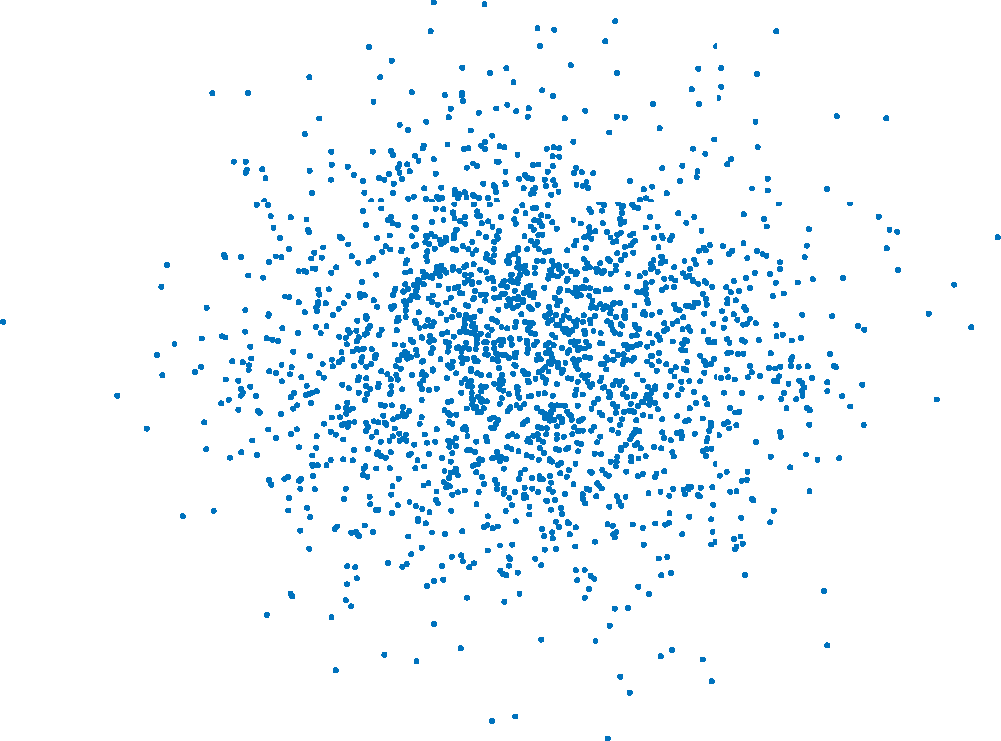
\includegraphics[width=0.4\textwidth]{figures/mvnrnd1}}
	\hfill
	\subfloat[$\displaystyle \begin{bmatrix} 1/10 & 0 \\ 0 & 1 \end{bmatrix}$]{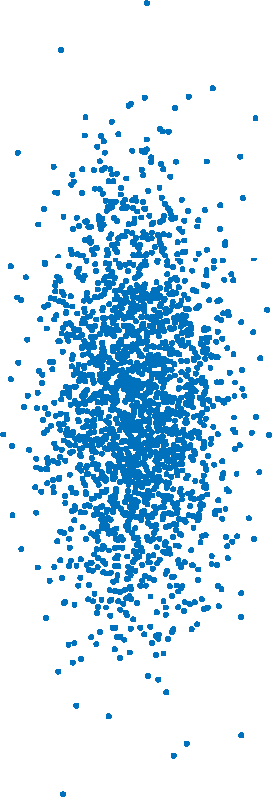
\includegraphics[width=0.1\textwidth]{figures/mvnrnd2}}
	\hfill
	\subfloat[$\displaystyle \begin{bmatrix} 0.7 & 0.3 \\ 0.3 & 0.4 \end{bmatrix}$]{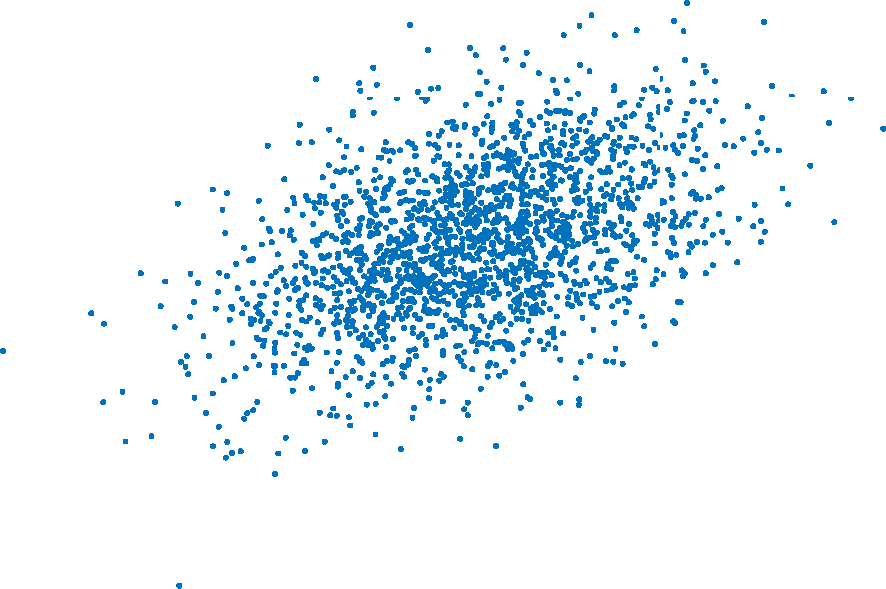
\includegraphics[width=0.4\textwidth]{figures/mvnrnd3}}
\end{figure}
\end{frame}



\begin{frame}
\frametitle{Analyse en composantes principales}
Comment trouver le sous-espace?

Deux critères équivalents:
\begin{itemize}[label=\tiny$\blacksquare$]
	\item minimiser l'erreur quadratique moyenne
	$$
		\min \frac{1}{N} \sum_{i=1}^N \norm{\mathbf{x}_i - \tilde{\mathbf{x}}_i}^2
	$$
	où $\tilde{\mathbf{x}}_i$ sont les données projetées (vu comme des vecteurs de $\RR^d$)
	
	\item maximiser la variance (empirique) \alert{totale} des données projetées
	$$
	\begin{aligned}
		%\max \frac{1}{N-1}\sum_{i=1}^N\sum_{j=1}^d (z_j^{(i)} - \bar{z}_j)
		\max \sum_{j=1}^{d'} \mathbf{u}_j^\top \widehat{\mathbf{C}} \mathbf{u}_j = \frac{1}{N-1}\sum_{j=1}^{d'} \sum_{i=1}^N \abs{\mathbf{u}_j^\top(\mathbf{x}_i - \bar{\mathbf{x}})}^2 &= \frac{1}{N-1}\sum_{i=1}^N \norm{\mathbf{U}^\top (\mathbf{x}_i - \bar{\mathbf{x}})}^2 \\
		&= \frac{1}{N-1}\sum_{i=1}^N\norm{\mathbf{z_i} - \bar{\mathbf{z}}}^2
	\end{aligned}
	$$
	où $\mathbf{z}_i$ sont les données projetées (vu comme des vecteurs de $\RR^{d'}$)
\end{itemize}
\end{frame}




\begin{frame}
\frametitle{Equivalence des deux critères}

On a
\begin{align}
	\norm{\mathbf{x}_i - \tilde{\mathbf{x}}_i}^2 
		&= \norm{\mathbf{x}_i - \bar{\mathbf{x}}}^2 + \norm{\bar{\mathbf{x}} - \tilde{\mathbf{x}}_i}^2 \tag{Pythagore}\\
		&= \mathrm{cste} + \norm{\mathbf{U}^\top(\bar{\mathbf{x}} - \tilde{\mathbf{x}}_i)}^2 \tag{orthogonalité}\\
		&= \mathrm{cste} + \norm{\mathbf{z_i} - \bar{\mathbf{z}}} \tag{$\mathbf{U}^\top\mathbf{x}_i=\mathbf{U}^\top\tilde{\mathbf{x}}_i$}
	\end{align}
\end{frame}



\begin{frame}
\frametitle{PCA et SVD}

Considérons la SVD de la matrice des données centrées $\mathbf{\underline{X}} = \widehat{\mathbf{U}} \widehat{\bm{\Sigma}} \widehat{\mathbf{V}}$

$$
		\frac{1}{N-1}\sum_{j=1}^{d'} \mathbf{u}_j^\top \widehat{\mathbf{U}}\widehat{\bm{\Sigma}}^2 \widehat{\mathbf{U}}^\top \mathbf{u}_j = \frac{1}{N-1}\sum_{j=1}^{d'}\sum_{i=1}^d \sigma_i^2\abs{\hat{\mathbf{u}}_i^\top \mathbf{u}_j}^2 \leq \frac{d'}{N-1}\sum_{i=1}^d \sigma_i^2
	$$
	avec égalité si $\mathbf{u}_j = \hat{\mathbf{u}}_j$ pour tout $j=1,\ldots,d'$.
	\vfill
	
	\begin{tcolorbox}
	Une base orthogonale du sous-espace optimal est donné par les $d'$ premiers vecteurs singuliers gauches de la matrice $\underline{\mathbf{X}}$.
	\end{tcolorbox}
	\vfill
	Les variances selon chaque direction sont liées aux (carrés des) valeurs singulières.
\end{frame}


\begin{frame}
\frametitle{Analyse en composantes principales}


\begin{figure}
	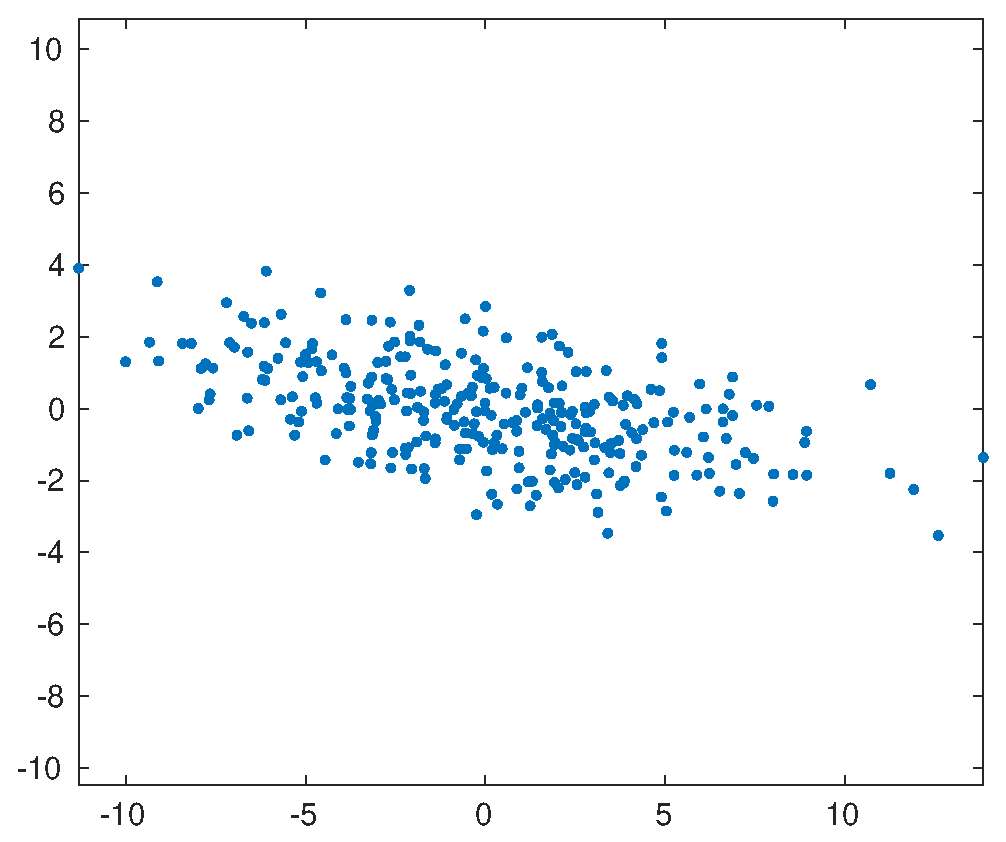
\includegraphics[width=0.45\textwidth]{figures/pca-dataset}
	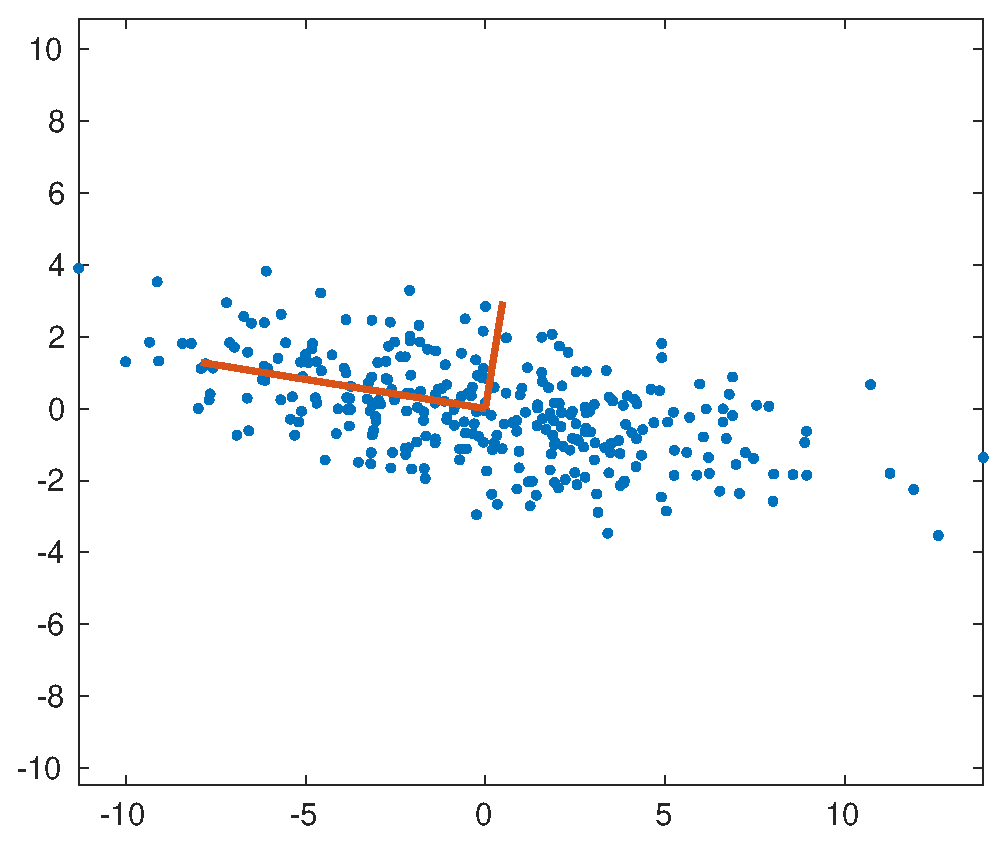
\includegraphics[width=0.45\textwidth]{figures/pca-axes}
\end{figure}

Composantes principales = vecteurs singuliers de la matrice de covariance

\end{frame}

%
%%\section{Factorisation en matrices non-negatives (NMF)}
%
%\section[NMF]{Factorisation en matrices non-négatives (NMF)}
%
%
%\begin{frame}[noframenumbering,plain]{Plan}
%\tableofcontents[currentsection]
%\end{frame}
%
%
%
%\begin{frame}
%\frametitle{Factorisation en matrices non-négatives (NMF)}
%		 \begin{center}
%		
\includegraphics[width=6cm]{figures/keep-calm-and-be-positive.eps}
%	\end{center}
%\end{frame}
%
%
%
%\begin{frame}
%\frametitle{Exemple: analyse de mélanges par spectroscopie}
%
%
%\begin{itemize}[label=\tiny$\blacksquare$]
%	\item Spectrocopie: mesure de la réponse lumineuse d'un tissu après excitation (par exemple laser)
%	\begin{itemize}[label=-]
%	\item { Un spectre mesuré est une combinaison linéaire des spectres des composantes pures ($\lambda$)}
%	\item { Acquisition de spectres dans différentes conditions physico-chimiques ($x$)}
%	\end{itemize}
%\end{itemize}
%
%\vspace*{.5cm}
%\begin{minipage}{0.25\textwidth}
%    \begin{center}
%    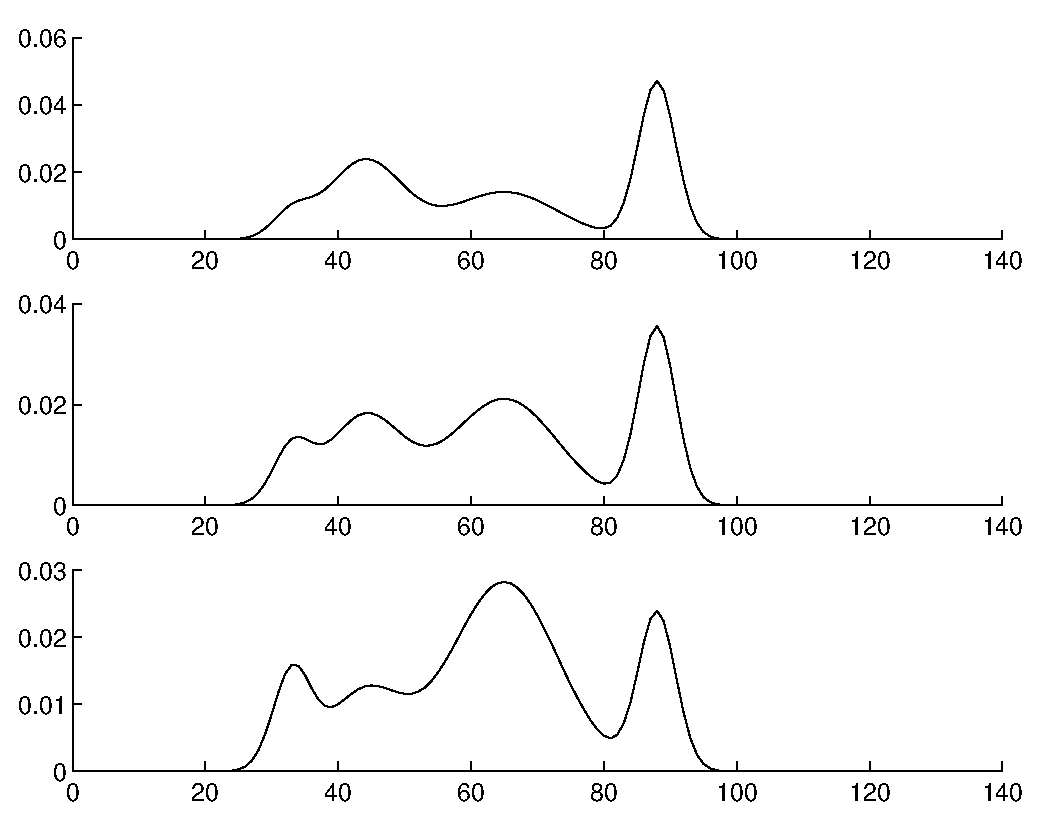
\includegraphics[width=3cm]{figures/melang.eps}
%    \end{center}
%\end{minipage}
%%
%\begin{minipage}{0.4\textwidth}
%$ \quad \quad = \quad  \left[ \begin{array}{ c c}
%  2/3    &   1/3 \\
%  1/2    &   1/2 \\
%  1/3    &   2/3
%\end{array}
%\right] \cdot $
%\end{minipage}
%%
%\begin{minipage}{0.25\textwidth}
%    \begin{center}
%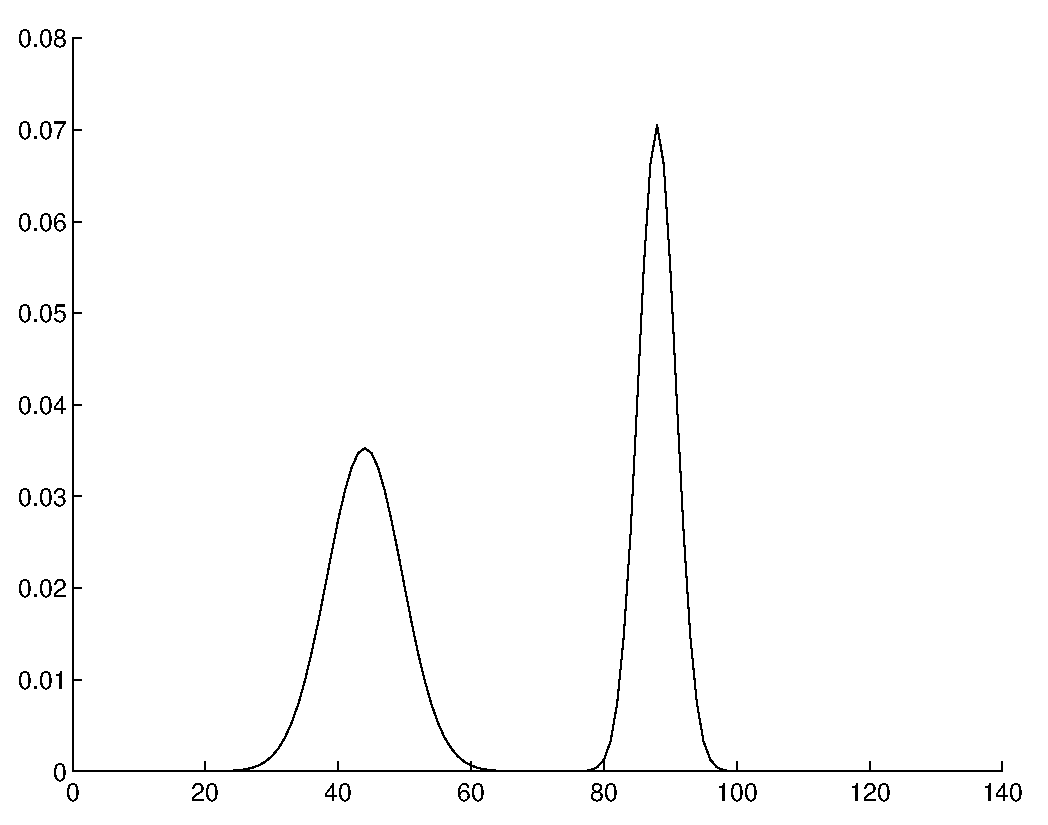
\includegraphics[height=1cm]{figures/S1.eps}\\ \vspace*{.5cm}
%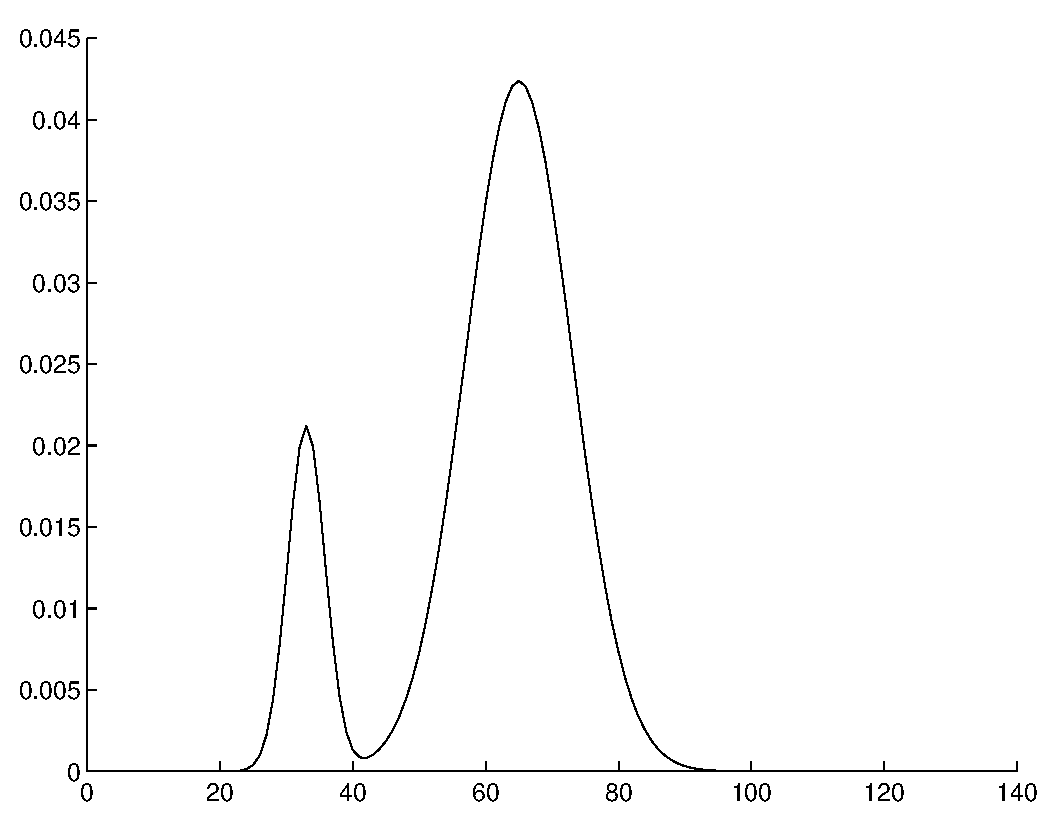
\includegraphics[height=1cm]{figures/S2.eps}
%    \end{center}
%\end{minipage}\\[5ex]
%\begin{center}
%Modèle de mélange instantané
%$$\tcbhighmath{
%\mathbf{X}(x,\lambda) = \sum_k \mathbf{a}_k(x) \mathbf{s}_k(\lambda)}
%$$
%
%Les valeurs sons positives!
%\end{center}
%\end{frame}
%
%
%\begin{frame}
%\frametitle{Séparation de sources}
%\begin{itemize}[label=\tiny$\blacksquare$]
%\item Analyse de données massives (Big Data)
%\item Bioinformatique
%\item Apprentissage statistique (Machine Learning)
%\item \textbf{Chimiometrie}
%\item \textbf{Imageries hyperspectrales} : télédétection, microscopie, ...
%\end{itemize}	  
%\end{frame}
%
%
%
%
%\begin{frame}
%\frametitle{Modèle de mélange instantané}
%$$
%\mathbf{X} = \mathbf{A} \, \mathbf{S}^T
%$$
%avec
%\\[2ex] 
%$\mathbf{X}$ : $(m \times n)$ matrice de données
%
%$\mathbf{A}$ : $(m \times p)$ matrice de mélange \emph{à estimer}
%
%$\mathbf{S}$ : $(n \times p)$ matrice source \emph{à estimer}
%\\[2ex] 
%{\bf Contrainte de non-negativité}
%\begin{equation*}
% \label{eq.2} \mathbf{A} \geq 0 \, \text{ et } \, \mathbf{S} \geq 0
%\end{equation*}
%\\[2ex] 
%{\bf $\Rightarrow$ Factorisation en matrices non-negatives (NMF) }
%
%\end{frame}
%
%
%\begin{frame}
%\frametitle{Factorisation en matrices non-negatives (NMF)}
%\begin{center}
%%\Large
%\textbf{Unicité ?}
%\end{center}
%
%\begin{itemize}
%\item \textbf{Quelles sont les conditions} sur $\mathbf{S}$ et
%$\mathbf{A}$ pour que la \textbf{NMF} de $\mathbf{X}$ \textbf{soit unique}?
%\item Si la solution n'est pas unique, quelle est l'ensemble des solutions admissibles ?
%\item Comment réduire l'ensemble des solutions admissibles?
%\end{itemize}
%\begin{center}
%%\Large
%\textbf{Algorithmes ?}
%\end{center}
%\begin{itemize}
%\item Estimation conjointe de $\mathbf{A} \geq 0 \, \text{ et } \, \mathbf{S} \geq 0$ : ALS, NMF,  ALS régularisée, NMF régularisée, méthodes Bayésiennes ...
%\item Méthodes géométriques : N-Findr, Minimum Volume Enclosing Simplex, ...
%\end{itemize} 
%%\begin{center}
%%\Large
%%{\bf Hypothèses}
%%\end{center}
%
%%\begin{itemize}
%%\item Existance de la NMF
%%\item Le rang de la factorisation est connue et rang$_+$ = rang
%%\end{itemize}
%\end{frame}
%
%%5%%%%%%%%%%%%%%%%%%%%%%%%%%%%%%%%%%%%%%%%%%%%%%%%%%%%%%%%%%%%%%%%%%%%%%%%%%%%%%%%%%%%%%%
%%\section[Unicité de la NMF]{NMF: unicité et solutions admissibles}
%\begin{frame}
%\frametitle{Unicité et solutions admissibles: bases}
%		 \begin{center}
%		
\includegraphics[width=6cm]{figures/keep-calm-and-be-unique.eps}
%	\end{center}
%\end{frame}
%
%\begin{frame}
%%5%%%%%%%%%%%%%%%%%%%%%%%%%%%%%%%%%%%%%%%%%%%%%%%%%%%%%%%%%%%%%%%%%%%%%%%%%%%%%%%%%%%%%%%
%\frametitle{Indéterminations}
%$\mathbf{A}$ et $\mathbf{S}$ sont des matrices de rang $p$  (rang colonne plein)
%$$
%\mathbf{A} \, \mathbf{S}^T = \mathbf{\tilde A} \, \mathbf{\tilde S}^T
%$$
%si et seulement si
%$$
% \exists \, \mathbf{T} (p \times p) \text{ inversible}
%\text{ telle que }
%\begin{cases}
% &\mathbf{\tilde A}  = \mathbf{A} \mathbf{T}^{-1}\\
% &\mathbf{\tilde S}  = \mathbf{S}\mathbf{T} ^T \Leftrightarrow \mathbf{\tilde S}^T  = \mathbf{T} \mathbf{S}^T  \\
%\end{cases}
%$$
%
%\textbf{Quelles sont les conditions sur $\mathbf{S,A}$ et $\mathbf{T}$
%qui permettent de garantir que $\mathbf{\tilde A}$ et $\mathbf{\tilde
%S}$ sont non-negatives?}\end{frame}
%%6%%%%%%%%%%%%%%%%%%%%%%%%%%%%%%%%%%%%%%%%%%%%%%%%%%%%%%%%%%%%%%%%%%%%%%%%%%%%%%%%%%%%%%%
%
%
%\begin{frame}
%\frametitle{Indéterminations triviales}
%\begin{center}
%\alert{\textbf{Indéterminations d'échelle}}
%\end{center}
%$$
% \mathbf{T} = \mathrm{Diag}(\lambda_1,...,\lambda_p) \text{ avec } \lambda_i>0,
% \forall i =1,...,p, \;  \Rightarrow \; \mathbf{\tilde S} \geq 0 \; \text{et} \; \mathbf{\tilde A} \geq 0.
%$$\\[3ex]
%Normalisation de $\mathbf{A}$ ou $\mathbf{S} $ (par exemple Sum to One)
%\\[6ex]
%
%\begin{center}
%\alert{\textbf{Indéterminations d'ordre}}
%\end{center}
%
%\begin{center}
%$\mathbf{T}$ matrice de permutation de ligne $\Rightarrow$
%$\mathbf{T}^{-1}$ matrice de permutation de colonne $\Rightarrow \;
%\mathbf{\tilde S} \geq 0 \; \text{and} \; \mathbf{\tilde A} \geq 0$.
%\\[3ex]
%\end{center}
%%L'indice est arbitraire !
%
%\end{frame}
%
%\begin{frame}
%\frametitle{Cas de 2 sources}
%
%\begin{equation*}
%\mathbf{A} = \left[\mathbf{a}_1 \; \mathbf{a}_2\right], \quad \mathbf{S} = \left[\mathbf{s}_1 \; \mathbf{s}_2\right],\quad  \mathbf{X} = \mathbf{A}\mathbf{S}^T =\tilde{\mathbf{A}}{\tilde{\mathbf{S}}}^T 
%\end{equation*}
%
%\alert{\textbf{Indéterminations d'ordre}}
%\[
%\bm{\Pi} =\bm{\Pi}^{-1} =\bm{\Pi}^{T} = \begin{bmatrix} 0 & 1 \\ 1 & 0
%\end{bmatrix}
%\]
%permutation des colonnes:
%\[
%\tilde{\mathbf{A}} =\mathbf{A} \bm{\Pi} = \left[\mathbf{a}_2 \; \mathbf{a}_1\right], \quad \tilde{\mathbf{S}} =\mathbf{S} \bm{\Pi} = \left[\mathbf{s}_2 \; \mathbf{s}_1\right]
%\]
%
%\alert{\textbf{Indéterminations d'échelle}}
%\[
%\bm{\Lambda} = \bm{\Lambda}^{\T} = \begin{bmatrix} \alpha & 0 \\ 0 & \beta
%\end{bmatrix},\quad \alpha,\beta \ge 0 
%\]
%\[
%\tilde{\mathbf{A}} = \mathbf{A} \bm{\Lambda}^{-1} = \left[\frac{1}{\alpha}\mathbf{a}_1 \; \frac{1}{\beta}\mathbf{a}_2\right],\quad \tilde{\mathbf{S}} = \mathbf{S} \bm{\Lambda}^{\T} =  \left[{\alpha}\mathbf{s}_1 \; {\beta}\mathbf{s}_2\right]
%\]
%
%
%
%
%\end{frame}
%
%
%%7%%%%%%%%%%%%%%%%%%%%%%%%%%%%%%%%%%%%%%%%%%%%%%%%%%%%%%%%%%%%%%%%%%%%%%%%%%%%%%%%%%%%%%%
%\begin{frame}
%\frametitle{Unicité essentielle}
%
%
%\begin{itemize}[label=\tiny$\blacksquare$]
%\item Une paire $(\mathbf{A},\mathbf{S})$ est une solution admissible si
%$\mathbf{A}$ et $\mathbf{S}$ sont des matrices non-negatives dont le produit donne  $\mathbf{X}$.
%\\[2ex]
%
%\begin{tcolorbox}%[width=1.03\textwidth]
%\item[]\begin{center}
%\textbf{Unicité essentielle}
%\end{center}
%Soit $\mathbf{X}$ une matrice admettant la NMF
%$\mathbf{X}=\mathbf{A} \, \mathbf{S}^T$. On dit que la solution est essentiellement unique  si les seules indéterminations sont les indéterminations d'ordre et d'échelle.
%\end{tcolorbox}
%
%\item Dans le cas de deux sources, \ie
%\begin{equation*}
%     \mathbf{A} = \left[\mathbf{a}_1 \; \mathbf{a}_2\right] \quad \mathbf{S} = \left[\mathbf{s}_1 \; \mathbf{s}_2\right]
%\end{equation*}
%on peut montrer que la NMF est essentiellement unique.
%\end{itemize}
%\end{frame}
%
%%%8%%%%%%%%%%%%%%%%%%%%%%%%%%%%%%%%%%%%%%%%%%%%%%%%%%%%%%%%%%%%%%%%%%%%%%%%%%%%%%%%%%%%%%%
%%\begin{frame}
%%\frametitle{Unicité essentielle: cas de 2 sources}
%%\begin{equation*}
%%     \mathbf{A} = \left[\mathbf{a}_1 \; \mathbf{a}_2\right] \quad \mathbf{S} = \left[\mathbf{s}_1 \; \mathbf{s}_2\right]
%%\end{equation*}
%%\\[2ex]
%%$\mathbf{a}_1,\mathbf{a}_2$ : vecteurs de dimension $(m,1)$ ;\\
%%$\mathbf{s}_1,\mathbf{s}_2$ : vecteurs de dimension $(n,1)$.
%%\\[2ex]
%%\begin{equation*}
%%\mathbf{T}(\alpha,\beta) = \left[
%%\begin{array}{cc}
%%1-\alpha & \alpha \\
%%\beta      & 1-\beta
%%\end{array}
%%\right]
%% \; \Rightarrow \;
%%\mathbf{T}^{-1}(\alpha,\beta) = \dfrac{1}{1 - \alpha - \beta}\left[
%%\begin{array}{cc}
%%1-\beta   & -\alpha  \\
%%-\beta    & 1-\alpha
%%\end{array}
%%\right].
%%\end{equation*}
%%\\[2ex]
%%$\alpha+\beta<1$ $\Rightarrow$ pas d'indétermination d'ordre et $\mathbf{T}$ inversible ;\\
%%$\sum\limits_{i=1}^p t_{ji} = 1$ $\Rightarrow$ pas d'indétermination d'échelle.
%%
%%\end{frame}
%%%9%%%%%%%%%%%%%%%%%%%%%%%%%%%%%%%%%%%%%%%%%%%%%%%%%%%%%%%%%%%%%%%%%%%%%%%%%%%%%%%%%%%%%%%
%%\begin{frame}
%%
%%\begin{center}
%%\frametitle{Solutions admissibles }
%%\end{center}
%%
%%\begin{equation*}
%%\begin{cases}
%% \mathbf{\tilde S}^T = \mathbf{T}(\alpha,\beta) \, \mathbf{S}^T; \\
%% \mathbf{\tilde A} = \mathbf{A}\, \mathbf{T}^{-1}(\alpha,\beta);
%% \end{cases}
%%\end{equation*}
%%\vskip5mm
%%\begin{multicols}{2}
%%\begin{center}
%%$\alpha \in [\alpha_{\min},\alpha_{\max}]$
%%$$
%%  \alpha_{\min} = - \underset{k \in \mathbb{K}_1}{\min} \left\{\dfrac{s_{k1}}{s_{k2}-s_{k1}}\right\}
%%$$
%%$$
%%  \alpha_{\max} = \underset{\ell}{\min} \left\{\dfrac{a_{\ell2}}{a_{\ell1} + a_{\ell2}}\right\}
%%$$
%%%\vskip-10mm
%%$$
%% \mathbb{K}_1  = \left\{k \in \{1,...,n\}; s_{k2} > s_{k1}\right\}.
%%$$
%%\end{center}
%%\vskip10mm
%%\begin{center}
%% $\beta \in [\beta_{\min},\beta_{\max}]$.
%%$$
%%   \beta_{\min} = - \underset{k \in \mathbb{K}_2}{\min} \left\{ \dfrac{s_{k2}}{s_{k1}- s_{k2}}\right\}
%%$$
%%$$
%%   \beta_{\max} = \underset{\ell}{\min} \left\{\dfrac{a_{\ell1}}{a_{\ell1} + a_{\ell2}}\right\}
%%$$
%%%\vskip-10mm
%%$$
%% \mathbb{K}_2 = \left\{k \in \{1,...,n\}; s_{k1} > s_{k2}\right\}
%%$$
%%\end{center}
%%\end{multicols}
%%\vskip-10mm
%%
%%\end{frame}
%%%10%%%%%%%%%%%%%%%%%%%%%%%%%%%%%%%%%%%%%%%%%%%%%%%%%%%%%%%%%%%%%%%%%%%%%%%%%%%%%%%%%%%%%%%
%%\begin{frame}
%%
%%\begin{center}
%%\frametitle{Unicité}
%%\end{center}
%%La NMF de $\mathbf{X}$ selon
%%\begin{equation*}
%%    \mathbf{X} = \mathbf{A} \, \mathbf{S}^T \text{ with } \mathbf{A}  \geq 0, \mathbf{S}  \geq 0,
%%\end{equation*}
%%est unique ssi $\exists \;
%%(k_1,k_2,\ell_1,\ell_2)$, with $k_1 \neq k_2$ and $ \ell_1 \neq
%%\ell_2$, tels que
%%\begin{equation*}
%%\label{cond:2}
%%%
%%\begin{cases}
%% s_{k_1 1} = 0,    \text{ et } \, s_{k_1 2} \neq 0 , \\
%% s_{k_2 2} = 0,    \text{ et } \, s_{k_2 1} \neq 0 , \\
%% a_{\ell_11} = 0, \text{ et } \, a_{\ell_12} \neq 0 , \\
%% a_{\ell_22} = 0, \text{ et } \, a_{\ell_21} \neq 0. \\
%%\end{cases}
%%\end{equation*}
%%
%%\end{frame}
%%%11%%%%%%%%%%%%%%%%%%%%%%%%%%%%%%%%%%%%%%%%%%%%%%%%%%%%%%%%%%%%%%%%%%%%%%%%%%%%%%%%%%%%%%%
%%\begin{frame}
%%
%%\begin{center}
%%\frametitle{Exemple}
%%\end{center}
%%Inspiré de l'analyse de mélanges par spectroscopie
%%
%%\begin{figure}[h!]
%%\centering{
%%%
%%\[
%%\begin{array}{ccc}
%%\text{Spectres de sources} & \quad & \text{Abondance}\\
%%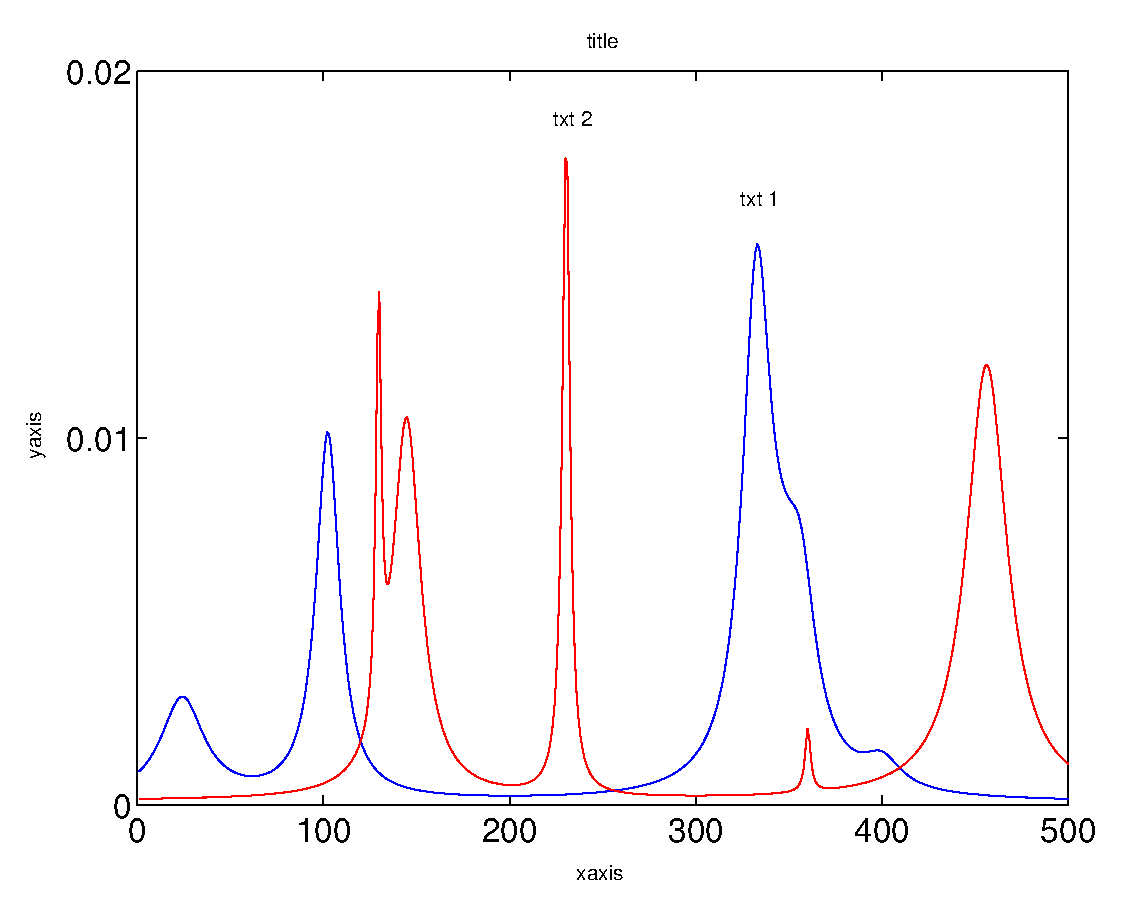
\includegraphics[height=3cm]{figures/sources} &&
%% 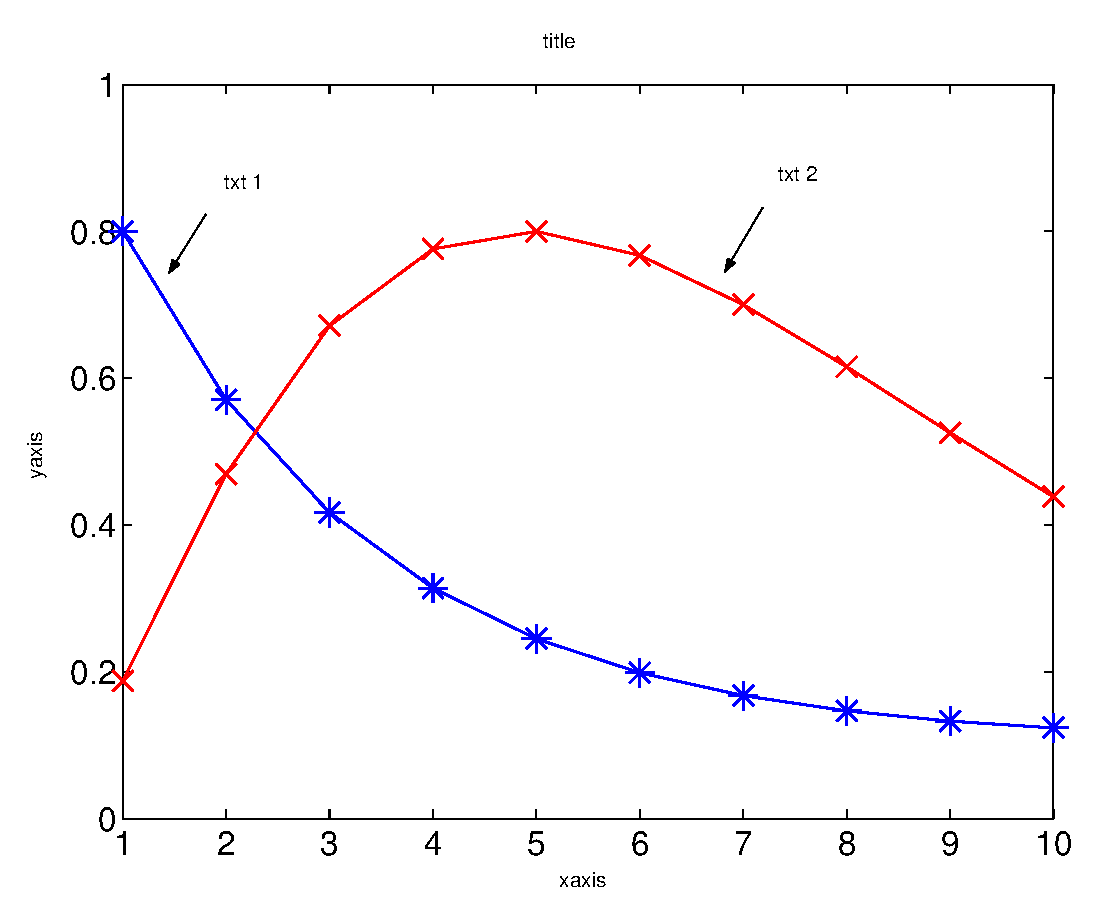
\includegraphics[height=3cm]{figures/mixcoef} \\
%%\text{Echantillons (longueur d'onde)} & & \text{Mesures}
%%\end{array}
%%\]
%%
%% \caption{\small Sources et abondances : \Blue{Composant 1} et \Red{Composant 2}}}
%% \end{figure}
%%
%%$\checkmark$ La condition d'unicité n'est pas satisfaite !
%%\end{frame}
%%%12%%%%%%%%%%%%%%%%%%%%%%%%%%%%%%%%%%%%%%%%%%%%%%%%%%%%%%%%%%%%%%%%%%%%%%%%%%%%%%%%%%%%%%%
%%\begin{frame}
%%
%%\begin{center}
%%\frametitle{Solutions admissibles }
%%\end{center}
%%\begin{gather*}
%% -0.0163 \leq \alpha \leq 0.1898, \quad  -0.0198 \leq \beta  \leq 0.1924.
%%\end{gather*}
%%
%%\begin{figure}[h!]
%%%
%%\centering{
%%\[
%%\begin{array}{ccc}
%%\text{Spectres de sources} & \quad & \text{Abondance}\\
%%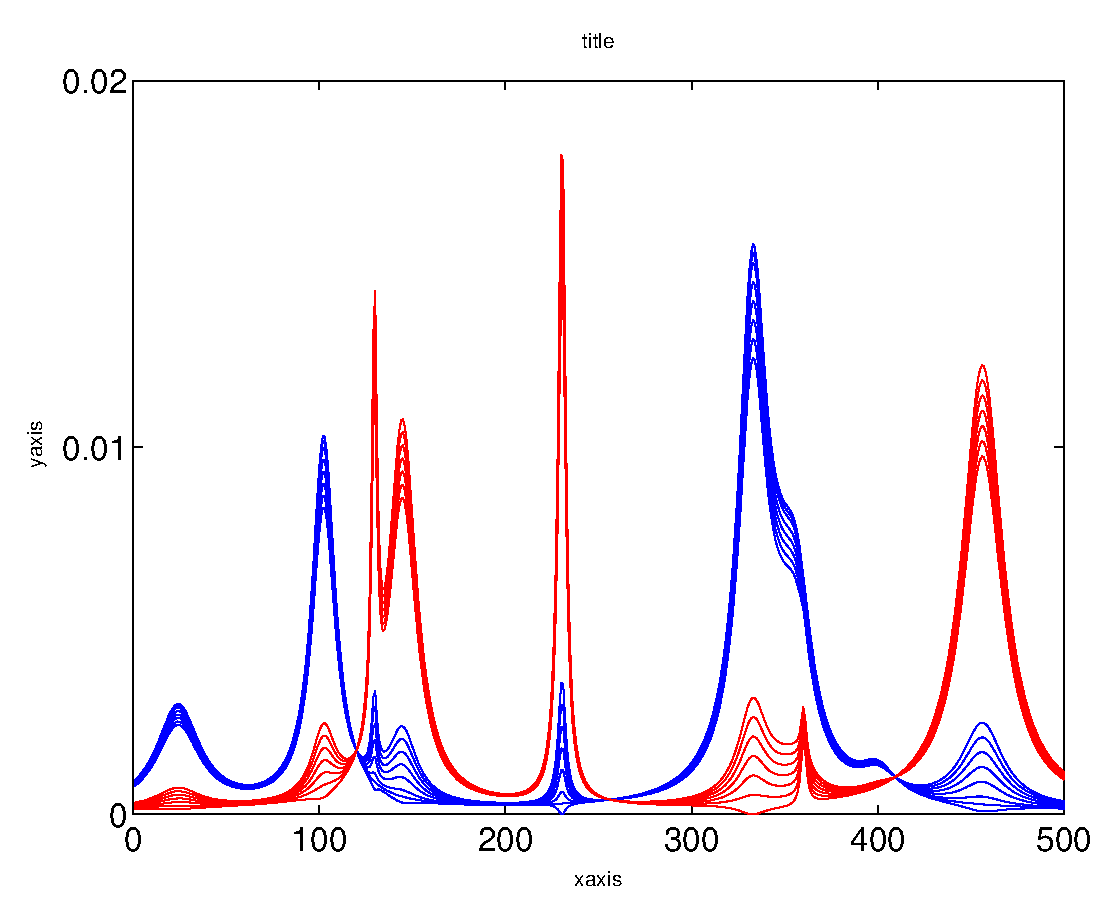
\includegraphics[height=3cm]{figures/sources_adm} &&
%% 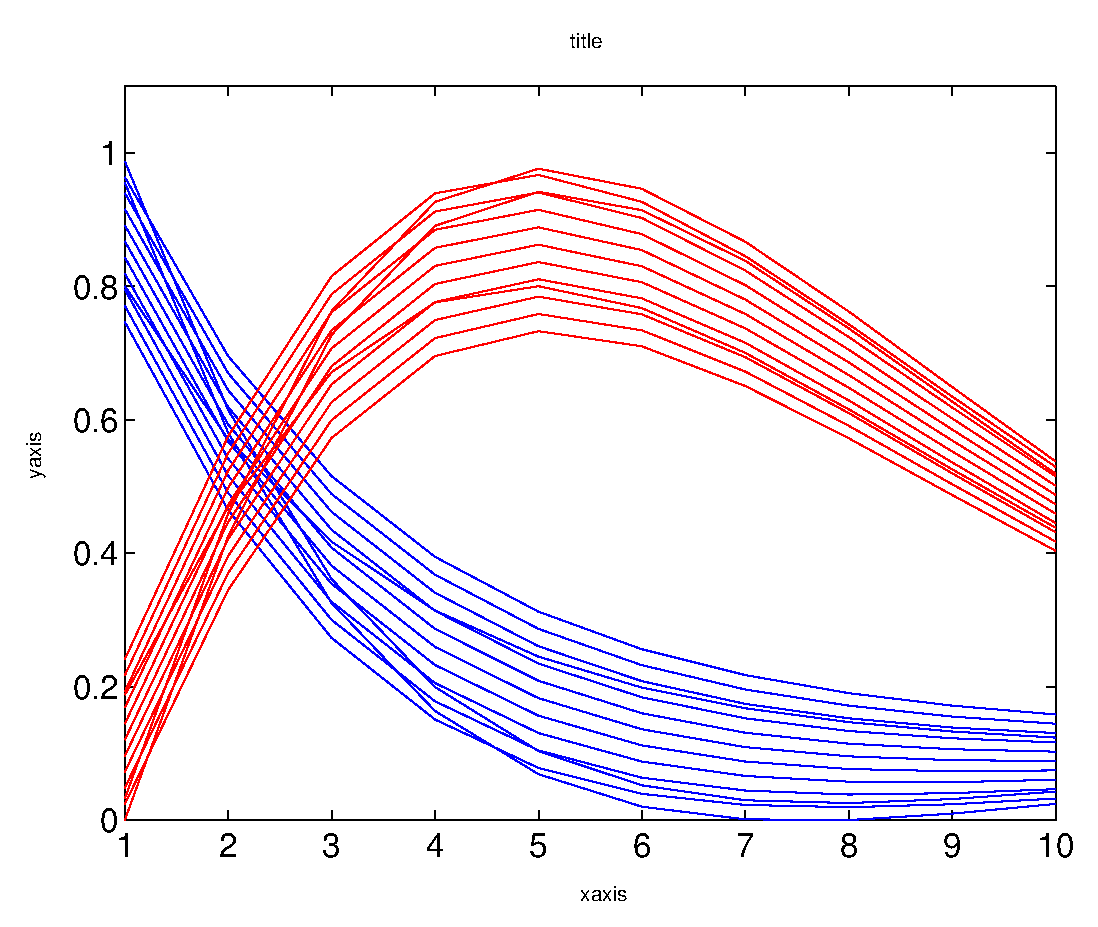
\includegraphics[height=3cm]{figures/mixcoef_adm} \\
%%\text{Echantillons (longueur d'onde)} & & \text{Mesures}
%%\end{array}
%%\]%
%% \caption{\small Solutions admissibles}}
%% \end{figure}
%
%%\end{frame}
%
%
%
%\begin{frame}
%\frametitle{Algorithmes de NMF}
%
%
%\begin{itemize}[label=\tiny$\blacksquare$]
%	\item Optimisation sous contraintes de positivité
%	\[
%		\min_{\mathbf{A}\geq 0, \mathbf{S}\geq 0} \quad  |\!|\mathbf{X} - \mathbf{A}\mathbf{S}^\top|\!|_F^2
%	\]
%	\item Problème non convexe $\rightarrow$ \alert{Minimisation alternée} de type \alert{"Alternate Least Squares" (ALS)}: MCR-ALS (Tauler), NMF (Lee \& Seung), ALS (Kim \& Park), HALS (Cichocki et al.)
%	\begin{align*}
%		&\mathbf{A}_{k+1} \leftarrow \min_{\mathbf{A}\geq 0} \quad  |\!|\mathbf{X} - \mathbf{A}\mathbf{S_k}^\top|\!|_F^2\\
%		&\mathbf{S}_{k+1} \,\leftarrow\min_{\mathbf{S}\geq 0} \quad  |\!|\mathbf{X} - \mathbf{A}_{k+1}\mathbf{S}^\top|\!|_F^2
%	\end{align*}
%	
%	\item Pour réduire d'avantage l'ensemble des solutions admissibles, on peut recourir à la régularisation ( = ajout de contraintes sur $\mathbf{A}$ et $\mathbf{S}$, par exemple parcimonie)
%\end{itemize}
%\end{frame}
%
%
%
%
%\section{Données tensorielles}
%
%\begin{frame}[noframenumbering,plain]{Plan}
%\tableofcontents[currentsection]
%\end{frame}
%
%\begin{frame}
%\frametitle{Applications}
%\begin{itemize}[label=\tiny$\blacksquare$]
%\item Analyse de données : co-clustering, graphes
%\item Apprentissage automatique : modélisation des distributions, réseaux de neurones
%\item Chimiométrie : MEEF, Microscopie Raman polarisée, RMN-ND
%\item Ingénierie biomédicale : EEG multivoie, ECG multivoie
%\item Biologie, environnement : gene array, bio-capteur, surveillance environnementale
%\item {Traitement d'antenne} : radar, astronomie, acoustique sous-marine, géophysique
%\item {Télécommunications} : MIMO, identification de canaux non-linéaires, ...
%\end{itemize}
%\end{frame}
%
%
%
%\begin{frame}
%\frametitle{Tenseurs}
%\begin{center}
%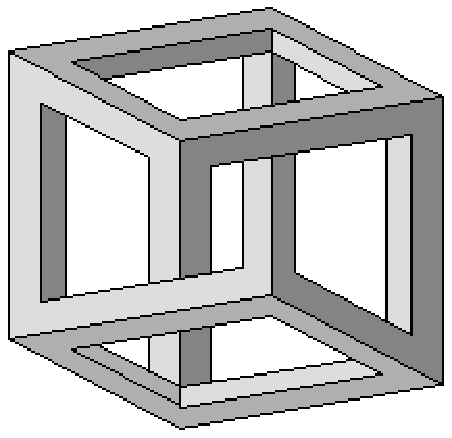
\includegraphics[width=6cm]{figures/cube}
%\end{center}
%\end{frame}
%
%
%
%
%
%\begin{frame}
%\frametitle{Tableaux multidimensionnels}
%\textbf{\large Fonction multivariable}
%$$
%\mathbf{v} = [v_1, \cdots, v_N]
%$$
%\begin{equation*}
%\begin{aligned}
%%\label{}
% x:  \ &  \mathbb{R}^N &\rightarrow &\ \ \mathbb{R}\\
%     &  \mathbf{v} &\mapsto &\ \ \ x(\mathbf{v} )
%\end{aligned}
%\end{equation*}
%\textbf{\large Cas discret} : échantillonnage de $x(\mathbf{v})$ sur une grille regulière $\rightarrow$ tableau multidimensionnel \\
%$$\mathcal{X}_{i_1 i_2 \cdots  i_N}$$
%On assimile un tenseur $\mathcal{X}$ à un tableau multidimensionnel. \\
%$N$ : ordre d'un tenseur (= nombre de modes)
%\end{frame}
%
%
%
%
%
%
%\begin{frame}\frametitle{Exemples et notation}
%\begin{itemize}
%\item ($N=0$) Scalaire $s$ 
%\item ($N=1$) vecteur $\mathbf{v}=[v_i]$ 
%\item ($N=2$) matrice $\mathbf{M}=[m_{ij}]$ 
%\item ($N \ge 3$) tenseur $\mathcal{T}= [t_{ijk}]_{i,j,k=1}^{I,J,K}$, $(\mathcal{T})_{ijk}= t_{ijk}$
%\[
%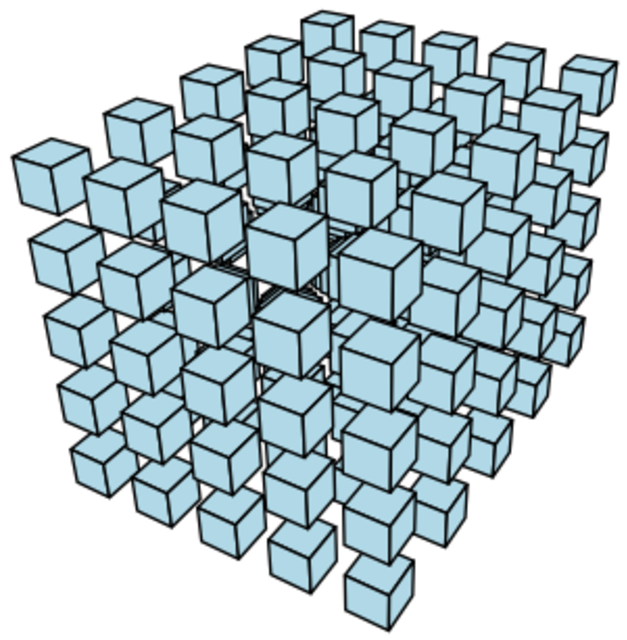
\includegraphics[height=0.3\textwidth]{figures/Tensor}
%\]
%\end{itemize}
%\end{frame}
%
%
%
%
%
%
%
%\begin{frame}
%\frametitle{Fibres, tranches (tenseur d'ordre 3)}
%\begin{itemize}
%\item Fibres:
%\[
%\begin{array}{ccccc}
%\text{colonnes} &\qquad& \text{lignes} &\qquad& \text{tubes}\\
%\calX_{:,j,k} && \calX_{i,:,k} &&  \calX_{i,j,:} 
%\end{array}
%\]
%\[
%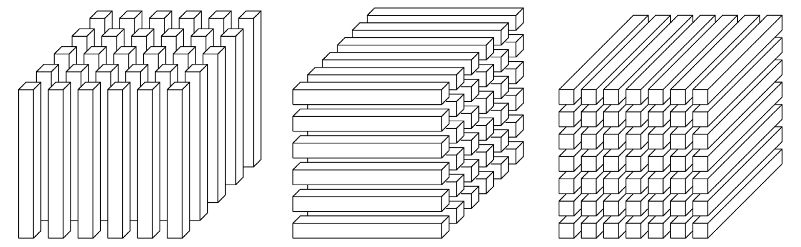
\includegraphics[height=2cm]{figures/fibers.png}
%\]
%\item Tranches:
%\[
%\begin{array}{ccccc}
%\text{horizontales} & \qquad&\text{latérales} & \qquad&\text{frontales} \\
%\calX_{i,:,:} & & \calX_{:,j,:} &&\calX_{:,:,k} 
%\end{array}
%\]
%\[
%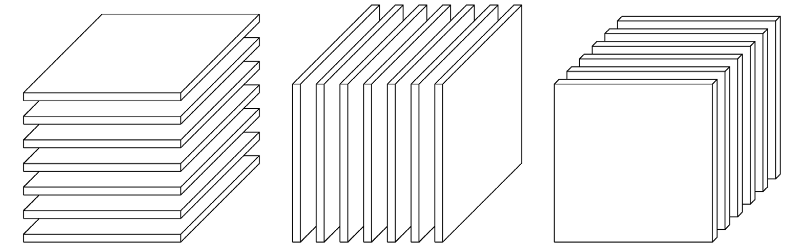
\includegraphics[height=2cm]{figures/slices.png}
%\]
%\end{itemize}
%%\begin{itemize}
%%\item Matrices are $2$-nd order tensors
%%\item Tensors are multilinear operators
%%\end{itemize}
%\end{frame}
%
%\begin{frame}\frametitle{Tenseur diagonal, tenseur symétrique}
%
%\begin{minipage}[l][5cm][c]{0.45\textwidth}
%\begin{center}
%\begin{tikzpicture}\begin{scope}[scale=1]
%\draw(0,0) rectangle (1,1);
%\draw(0,1) -- (0.5,1.5) -- (1.5,1.5) -- (1.5,0.5) --(1,0);
%\draw(1,1) -- (1.5,1.5);
%\draw(0.1,0.9) node (A) {\scriptsize \Blue{$1$}};
%\draw(0.4,0.8) node (A) {\scriptsize \Blue{$1$}};
%\draw(0.7,0.7) node (A) {\scriptsize \Blue{$\cdot$}};
%\draw(1.05,0.6) node (A) {\scriptsize\Blue{$\cdot$}};
%\draw(1.4,0.5) node (A) {\scriptsize \Blue{$1$}};
%\end{scope}\end{tikzpicture}
%\\[3.2ex]
%Tenseur diagonal
%$$
%(\mathcal{X})_{ijk} \neq 0 \text{ ssi } i =j=k
%$$
%\end{center}
%%
%\end{minipage}
%\begin{minipage}[l][5cm][c]{0.45\textwidth}
% \begin{center}
%\[
%{% !TEX root = UsevichGDRISIS2020.tex
\begin{tikzpicture}
\tikzstyle{p3} = [color = green!60!black]
\tikzstyle{p2} = [color = blue]
\tikzstyle{p1} = [color = red]
\tikzstyle{p0} = [color = black]

\begin{scope}[xscale= 0.75,yscale=0.75]
\tikzstyle{dot} = [draw,circle,minimum size=1.5mm,fill,inner sep=0mm]

\draw(0,0) node[dot,p1]          (v0001) {};
\draw(1,0) node[dot,p2]          (v0011) {};
\draw(0,1) node[dot,p0]          (v0000) {};
\draw(1,1) node[dot,p1]          (v0010) {};
\draw(0.5,0.5) node[dot,p2]      (v0101) {};
\draw(1.5,0.5) node[dot,p3]      (v0111) {};
\draw(0.5,1.5) node[dot,p1]      (v0100) {};
\draw(1.5,1.5) node[dot,p2]      (v0110) {};

\draw (v0000) -- (v0010) -- (v0011) -- (v0001) -- (v0000);
\draw (v0100) -- (v0110) -- (v0111) -- (v0101) -- (v0100);
\draw (v0000) -- (v0100);
\draw (v0010) -- (v0110) ;
\draw (v0001) -- (v0101);
\draw (v0011) -- (v0111) ;

\end{scope}
\end{tikzpicture}}
%\]
%\\[1.8ex]
%Tenseur (cubique) symétrique
%$$
%(\mathcal{X})_{ijk} = \mathcal{X}_{\sigma(ijk)}, \ \sigma : \text{permutation}
%$$
%\end{center}
%\end{minipage}
%\end{frame}
%
%
%\begin{frame}
%\frametitle{Dépliements}
%\textbf{Transformation d'un tenseur en une matrice } \\[2ex]
%Un tenseur $\mathcal{Y}$ peut se déplier de $N$ façons différentes : $\mathbf{Y}_{(n)}$
%\[
%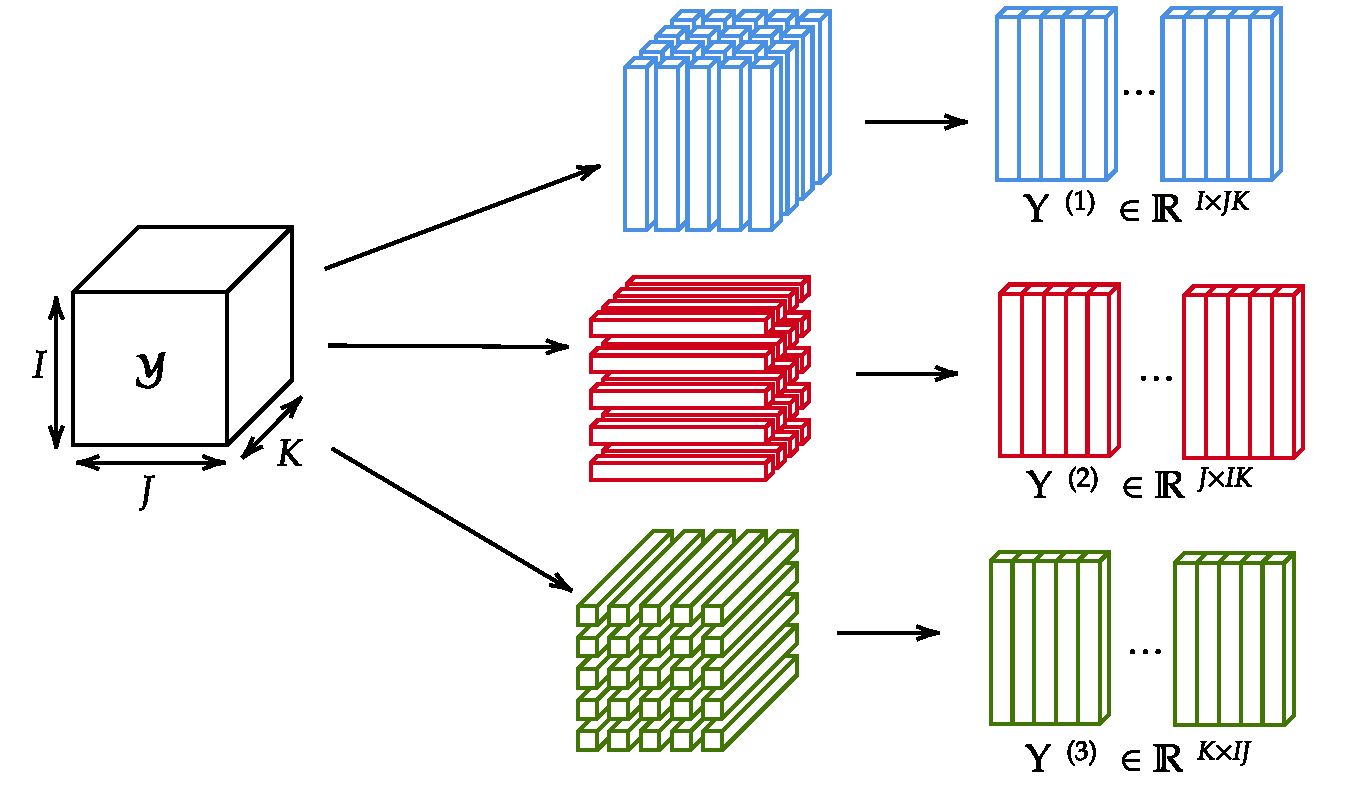
\includegraphics[height=5cm]{figures/unfold}
%\]
%\textbf{Transformation d'un tenseur en un vecteur}\quad
%$\mathbf{y} = \text{vec}(\mathcal{Y}) \ (I J K \times 1)$
%
%\textbf{\color{blue} Matlab (demo 1) }
%\end{frame}
%
%
%\begin{frame}
%\frametitle{Produits matriciels et tensoriels}
%\begin{center}
%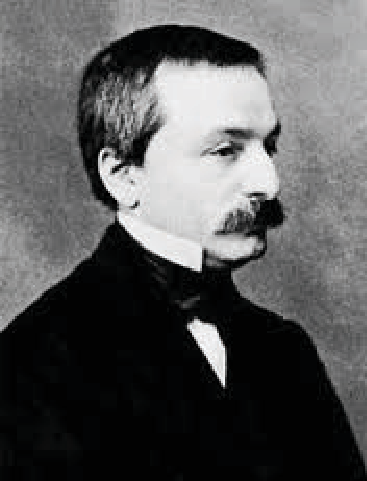
\includegraphics[width=2cm]{figures/Kron}
%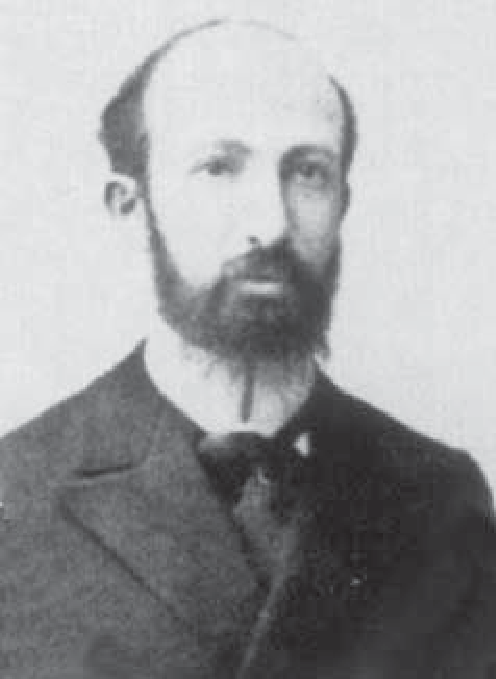
\includegraphics[width=2cm]{figures/Hadamard}
%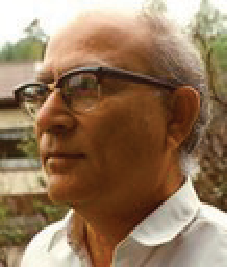
\includegraphics[width=2cm]{figures/Khatri}
%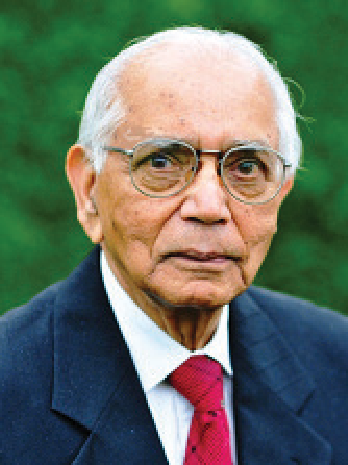
\includegraphics[width=2cm]{figures/Rao}
%\end{center}
%\begin{center}
%Kronecker, Hadamard, Khatri-Rao
%\end{center}
%\end{frame}
%%%%%%%%%%%%%%%%%
%
%
%\begin{frame}
%\frametitle{Produits matriciels et tensoriels (1)}
%\textbf{Notations}
%$$ \mathbf{A} = [\mathbf{a}_1 \cdots \mathbf{a}_R], \ (I \times R)
%\quad
%\mathbf{B} = [\mathbf{b}_1 \cdots \mathbf{b}_R], \ (J \times R)$$
%
%\textbf{Produit de Kronnecker}
%
%$$ \mathbf{A} \otimes  \mathbf{B}  =
% \left[   \begin{array}{ c c c}
%a_{11} \mathbf{B}    &  a_{12} \mathbf{B} & \cdots    \\
%a_{21} \mathbf{B}    &  a_{22}  \mathbf{B}& \cdots    \\
%                                             &  \vdots                                &     
%\end{array} \right]
%$$
%
%\textbf{Produit de Khatri-Rao}
% $$ \mathbf{A} \odot  \mathbf{B}  =  [\mathbf{a}_1 \otimes  \mathbf{b}_1 \cdots \mathbf{a}_R  \otimes  \mathbf{b}_R], \ (IJ \times R)$$
% 
%\textbf{Produit de Hadamard} (produit termes à termes)\\
%$\mathbf{A}, \mathbf{B}$ matrices de même dimension $(I \times J)$ 
%$$ \mathbf{A} \ast  \mathbf{B}  = [ a_{ij} b_{ij}] , (I \times J)$$
%\end{frame}
%%%%%%%%%%%%%%%%%%%%%%%%%%%%%%%%%%
%%%%%%%%%%%%%%%%%%%%%%%%%%%%%%%%%%%
%
%\begin{frame}
%\frametitle{Produits matriciels et tensoriels (2)}
%
%\textbf{Propriétés}\\
%
%\[
%\boxed{\text{vec}(\mathbf{A} \mathbf{X}  \mathbf{B}) = (\mathbf{B}^{T} \otimes \mathbf{A})\text{vec}(\mathbf{X})} 
%\]
%
%$$
%(\mathbf{A} \otimes  \mathbf{B}  ) (\mathbf{C} \otimes  \mathbf{D}  ) = \mathbf{A}   \mathbf{C}  \otimes \mathbf{B}   \mathbf{D} 
%$$
%
%$$
%(\mathbf{A} \otimes  \mathbf{B}  )^\dagger = \mathbf{A}^\dagger \otimes  \mathbf{B}^\dagger  
%$$
%
%
%$$
%(\mathbf{A} \odot  \mathbf{B}  )\odot \mathbf{C} = \mathbf{A} \odot (\mathbf{B}  \odot \mathbf{C} ) = \mathbf{A} \odot  \mathbf{B}  \odot \mathbf{C}
%$$
%
%$$
%(\mathbf{A} \odot  \mathbf{B} )^\top (\mathbf{A} \odot  \mathbf{B} ) = \mathbf{A}^\top \mathbf{A} \ast   \mathbf{B}^\top \mathbf{B}
%$$
%
%$$
%(\mathbf{A} \odot  \mathbf{B} )^\dagger = (\mathbf{A}^\top \mathbf{A} \ast   \mathbf{B}^\top \mathbf{B})^\dagger (\mathbf{A} \odot  \mathbf{B} )^\top
%$$
%
%
%
%$^\top$ : transposée\\
%$\dagger$: pseudoinverse
%
%\end{frame}
%%%%%%%%%%%%%%%%%%%%%%%%%%%%%%%%%%
%%%%%%%%%%%%%%%%%%%%%%%%%%%%%%%%%%%
%
%\begin{frame}
%\frametitle{Produits matriciels et tensoriels (3)}
%\textbf{Produit tensoriel }
%$$ 
%\mathbf{a} \circ \mathbf{b}, \ (I \times J),
%\quad  
%(\mathbf{a} \circ \mathbf{b})_{ij} = a_i  b_j\text{ \emph{i.e.} } \mathbf{a} \circ \mathbf{b} = \mathbf{a} \mathbf{b}^T, \text{ matrice de rang 1.}
%$$
%$$ 
%\mathbf{a} \circ \mathbf{b} \circ \mathbf{c}, \ (I \times J \times K),
%\quad  
%(\mathbf{a} \circ \mathbf{b} \circ \mathbf{c})_{ijk}  =  a_i  b_j c_k\text{ \emph{i.e.}  tenseur de rang 1.}
%$$
%
%\textbf{Produit n-mode}
%$$\mathbf{A}: \ (J \times I_n), \quad \mathcal{X}: \  (I_1 \times I_2  \cdots \times I_N )$$
%$$ \mathcal{X} \times_n A : \  (I_1 \times  \cdots \times I_{n-1} \times J \times I_{n+1} \dots \times I_N )$$
%$$
%(\mathcal{X} \times_n A )_{i_1\cdots i_{n-1} j i_{n+1}\cdots i_{N}}= \sum_{i_n = 1}^{I_1} x_{i_1 \cdots i_{N}} a_{j i_{n}}
%$$
%
%\textbf{\color{blue} Matlab (demo 2) }
%\end{frame}
%%2%%%%%%%%%%%%%%%%%%%%%%%%%%%%%%%%%%%%%%%%%%%%%%%%%%%%%%%%%%%%%%%%%%%%%%%%%%%%%%%%%%%%%%%
%
%\section{Décompositions tensorielles}
%
%
%\begin{frame}[noframenumbering,plain]{Plan}
%\tableofcontents[currentsection]
%\end{frame}
%
%\begin{frame}
%\frametitle{Décompositions tensorielles}
%\begin{center}
%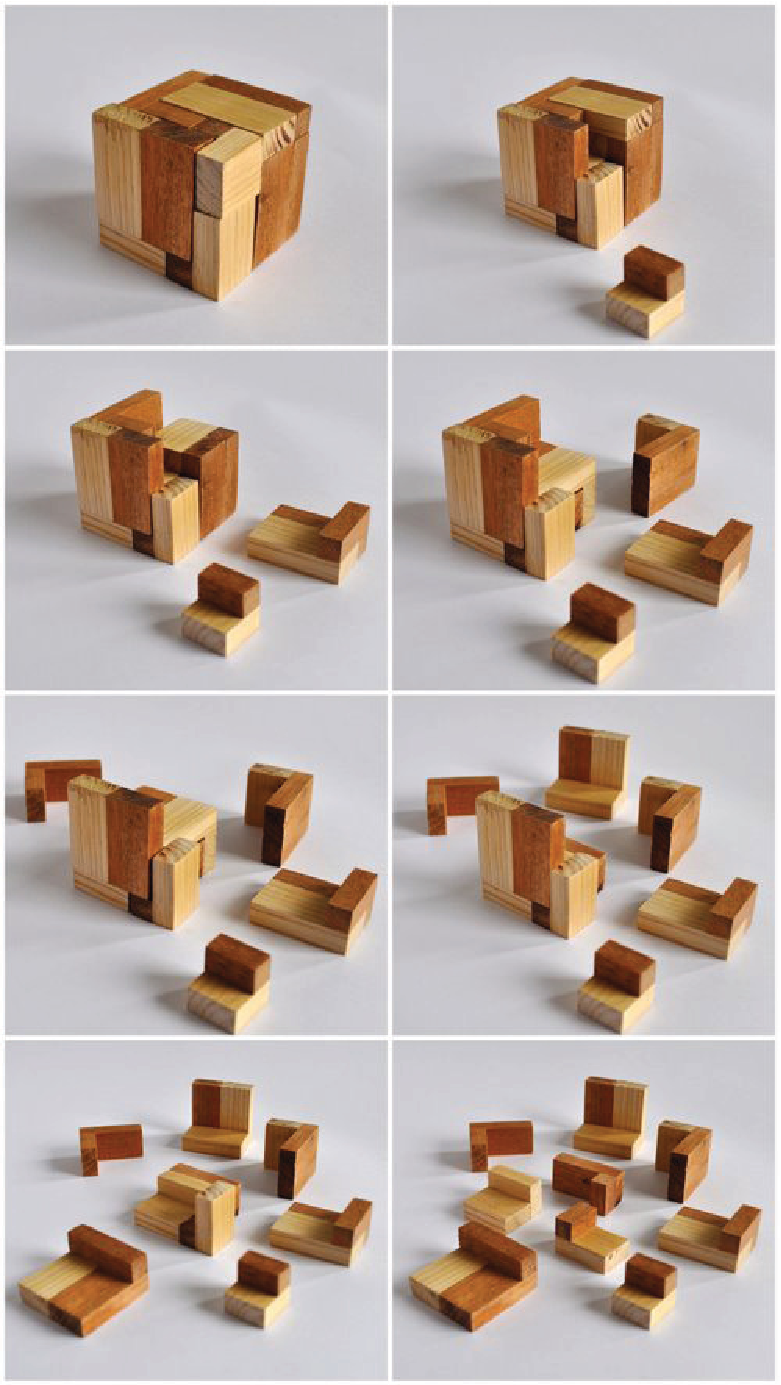
\includegraphics[width=4cm]{figures/cube_decompose}
%\end{center}
%\end{frame}
%
%
%\begin{frame}
%\frametitle{Rappel : rang matriciel}
%\[
%\mathbf{X} \in \mathbb{R}^{I \times J}, \quad \mathbf{X} = \sum_{r=1}^R  \mathbf{a}_{r} \mathbf{b}_{r}^T = \mathbf{A} \mathbf{B}^T
%\]
%\[
%\raisebox{-0.35\height}{\begin{tikzpicture}[scale=0.8]
%\draw(0,0.5) node (A) {$\mathbf{X}$};
%\draw(-1.1,0.5) node (eq) {\footnotesize ${I}$};
%\draw(0,1.4) node (eq) {\footnotesize ${J}$};
%\draw(-0.7,0) rectangle (0.7,1);
%\draw(1.1,0.5) node (eq) {${=}$};
%\draw(1.6,0) -- (1.6,1);
%\draw(1.6,0.5) node[fill=white] (a1) {{ $\bfa_1$}};
%\draw(1.7,1) -- (3.08,1);
%\draw(2.35,1) node[fill=white] (b1) {{\small $\bfb_1^{\T}\!\!$}};
%\draw(3.5,0.5) node () {{\small $+\; \cdots\;+$}};
%\draw(4.6,0) -- (4.6,1);
%\draw(4.6,0.5) node[fill=white] (a1) {{ $\bfa_R$}};
%\draw(4.7,1) -- (6.08,1);
%\draw(5.35,1) node[fill=white] (b1) {{\small $\bfb_R^{T}\!\!$}};
%\end{tikzpicture}}
%\raisebox{-0.35\height}{\begin{tikzpicture}[scale=0.8]
%%\draw(0,0.5) node (A) {$\mathbf{X}$};
%%\draw(-1.1,0.5) node (eq) {\footnotesize ${m}$};
%%\draw(0,1.4) node (eq) {\footnotesize ${n}$};
%%\draw(-0.8,0) rectangle (0.8,1.2);
%\draw(1.2,0.5) node (eq) {$=$};
%
%\draw(1.7,0.5) node (eq) {\footnotesize ${I}$};
%
%\draw(2,0) rectangle (2.6,1.2); %node {A};
%\draw(2.3,0.6) node (A) {$\mathbf{A}$};
%
%\draw(2.3,1.4) node (eq) {\footnotesize ${R}$};
%%\draw(5,0.5) node (eq) {\footnotesize$\quad+\,\cdots\,+\quad$};
%\draw(3.5,1.4) node (eq) {\footnotesize ${J}$};
%
%\draw(3,0.65) rectangle (4.2,1.2); %node {A};
%\draw(2.8,0.95) node (eq) {\footnotesize ${R}$};
%\draw(3.6,0.95) node (A) {$\mathbf{B}^{T}$};
%\end{tikzpicture}}
%\]
%
%\textbf{Rang d'une matrice} : 
%\begin{itemize}
%\item[1.] nombre minimal de matrices de rang 1 permettant de représenter $\mathbf{X}$
%\item[2.] taille minimale de la factorisation $\mathbf{A} \mathbf{B}^T $
%\end{itemize}
%
%%No
%%$\Rightarrow$ \textbf{Approximation de rang faible}\\[2ex]
%%\textbf{Indéterminations} : ordre, échelle, rotation
%%\begin{equation*} 
%%\mathbf{A} \mathbf{B}^T = (\mathbf{A} \mathbf{T}) ( \mathbf{T}^{-1}\mathbf{B}^T)  
%%= \tilde{\mathbf{A}} \tilde{\mathbf{B}}^T 
%%\end{equation*}
% \textbf{Contraintes} d'orthogonalité: SVD \quad $\mathbf{X} = \mathbf{U} \mathbf{\Sigma}\mathbf{V}^{T}$
%\\[2ex]
%
%
%\begin{tcolorbox}
%\textbf{Extension de la SVD} aux tenseurs depend de la définition du rang :
%\begin{itemize}
%\item[1.] Décomposition CP (canonique polyadique)
%\item[2.] Décomposition Tucker: HOSVD (Higher order SVD)
%\end{itemize}
%\end{tcolorbox}
%
%\end{frame}
%
%
%\begin{frame}
%\frametitle{Décomposition de Tucker d'un tenseur d'ordre 3}
%\begin{center}
%$[$Tucker, 1966$]$, $[$De Lathauwer 1997$]$\\[2ex]
%\end{center}
%$$(\mathcal{Y} )_{ijk}= \sum_{p=1}^{R_1} \sum_{q=1}^{R_2} \sum_{r=1}^{R_3} g_{pqr} u_{ip} v_{jq} w_{kr} $$
%$$\mathcal{Y} = \sum_{p=1}^{R_1} \sum_{q=1}^{R_2} \sum_{r=1}^{R_3} g_{pqr} \mathbf{u}_{p} \circ \mathbf{v}_{q}  \circ \mathbf{w}_{r} $$
%
%$$\mathcal{Y} = \mathcal{G} \times_1 \mathbf{U}  \times_2 \mathbf{V} \times_3 \mathbf{W} = [\![ \mathcal{G}, \mathbf{U}, \mathbf{V}, \mathbf{W} ]\!]$$
%\[
%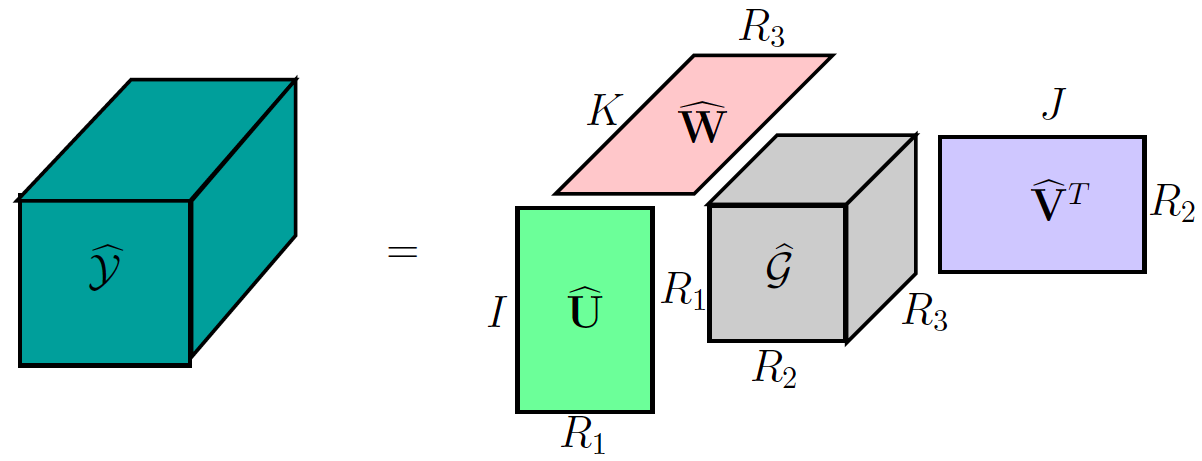
\includegraphics[height=2.5cm]{figures/tucker_exact}
%\]
%\begin{itemize}
%\item  $\mathcal{G}$ --- tenseur coeur
%\item $\mathbf{U}$, $\mathbf{V}$, $\mathbf{W}$ --- matrices facteurs
%\end{itemize}
%\end{frame}
%
%
%\begin{frame}
%\frametitle{Décomposition de Tucker d'un tenseur d'ordre N}
%$$\mathcal{X} = \mathcal{G} \times_1 \mathbf{A}^{(1)}  \times_2 \mathbf{A}^{(N)}  \cdots \times_N \mathbf{A}^{(N)}  = [\![ \mathcal{G}, \mathbf{A}^{(1)} , \cdots, \mathbf{A}^{(N)}  ]\!] $$
%\\[4ex]
%\textbf{ Non unicité de la décomposition de Tucker}\\
%$$\mathcal{X} = [\![ \mathcal{G} \times_1 \mathbf{T}_1  \times_2 \mathbf{T}_2 \times_3 \mathbf{T}_3, \mathbf{A}\mathbf{T}_1^{-1}, \mathbf{B}\mathbf{T}_2^{-1}, \mathbf{C} \mathbf{T}_3^{-1}]\!] $$
%%
%Contraintes : Orthogonalité des modes et du tenseur coeur 
%%
%$$\mathcal{X} =  [\![ \mathcal{G}, \mathbf{U}^{(1)} , \cdots, \mathbf{U}^{(N)}  ]\!] $$
%\\[4ex]
%
%\begin{tcolorbox}
%\textbf{n-rank} : rang colonne du tenseur déplié selon le mode $n$ : $R_n = \text{rank}(\mathbf{X}_{(n)})$
%\\[2ex]
%$\Rightarrow$  \textbf{rang multilinéaire} du tenseur: $(R_1,R_2,\ldots,R_N)$
%\end{tcolorbox}
%\end{frame}
%%procedure HOSVD(X,R1,R2, . . . , RN ) 
%%for n = 1,...,N do
%%A(n) ? Rn leading left singular vectors of X(n) 
%%end for
%%G?X×1A(1)T×2A(2)T···×N A(N)T
%%return G,A(1),A(2),...,A(N) end procedure
%
%\begin{frame}\frametitle{Algorithme HOSVD}
%
%
%\scalebox{.91}{ 
%\hspace*{1cm}
%\begin{algorithm*}[H]
% %\caption{\label{algo}CP-ALS(X,R)}
% \KwData{ Data $\mathcal{X}$, rank-$(R_1, \cdots R_N)$ }
%%\\[2ex]
% \For{$n = 1, \cdots, N$}{
%   	$[\mathbf{U}_n, \bm{\Lambda}, \mathbf{V}_n] = \text{svd}(\mathbf{X}_{(n)}, R_n)$
% }
% $\mathcal{G} = \mathcal{X} \times_1 \mathbf{U}_1^\top \cdots \times_N \mathbf{U}_N^\top$\\[2ex]
% \KwResult{$\mathcal{G}, \ \mathbf{U}_1 \cdots \mathbf{U}_N$}
%\end{algorithm*}
%}
%
%\textbf{Très proche d'une meilleure approximation de rang-$(R_1, \cdots R_N)$}
%
%[De Lathauwer 1997]
%\end{frame}
%
%\begin{frame}
%\frametitle{Décomposition CP d'un tenseur d'ordre 3}
%
%CP (canonique polyadique) : Candecomp/PARAFAC
%[Hitchkock, 1927] [Harshman, 1970-1972], [Carroll - Chang, 1970]
%
%\[
%\calX = \sum\limits_{r=1}^{R} \bfa_r \circ \bfb_r \circ \bfc_r, 
%\quad 
%\raisebox{-0.3\height}{\begin{tikzpicture}
%\begin{scope}[scale= 0.5]
%\draw(0.5,0.5) node (A) {$\mathcal{X}$};
%\draw(0,0) rectangle (1,1);
%\draw(0,1) -- (0.5,1.5) -- (1.5,1.5) -- (1.5,0.5) --(1,0);
%\draw(1,1) -- (1.5,1.5);
%
%\draw(2,0.8) node (eq) {$=$};
%\draw(6,0.8) node (eq) {$\quad+\,\cdots\,+\quad$};
%\end{scope}
%
%\begin{scope}[scale= 0.5,xshift=1cm]
%\draw(2,-0.2) -- (2,0.8);
%\draw(2.1,0.3) node[anchor=east] (s21) {\small {\footnotesize$\bfa_1$}};
%\draw(2.2,1) -- (3.2,1);
%\draw(2.8,1.2) node[anchor=north] (s22) {\small {\footnotesize$\bfb_1$}};
%\draw(2.2,1.2) -- (2.7,1.7);
%\draw(2.5,1.1) node[anchor=south east] (s23) {\small{\footnotesize$\bfc_1$}};
%\end{scope}
%
%\begin{scope}[scale= 0.5,xshift=6cm]
%\draw(2,-0.2) -- (2,0.8);
%\draw(2.1,0.3) node[anchor=east] (s21) {\small {\footnotesize$\bfa_R$}};
%\draw(2.2,1) -- (3.2,1);
%\draw(2.8,1.2) node[anchor=north] (s22) {\small {\footnotesize$\bfb_R$}};
%\draw(2.2,1.2) -- (2.7,1.7);
%\draw(2.5,1.1) node[anchor=south east] (s23) {\small {\footnotesize$\bfc_R$}};
%%\draw(1.9,1) node (g1) {\textcolor{red}{\small $c_r$}};
%\end{scope}
%\end{tikzpicture}}
%\]
%
%\begin{tcolorbox}[width=\textwidth]
%\textbf{rang tensoriel}  $\eqdef$ nombre minimal $R$ de tenseurs de rang 1 nécessaire pour représenter 
%
%\hfill $\mathcal{X}$.
%\end{tcolorbox}
% 
%  
% \vspace{2em}
% 
%Notation:  $\mathcal{X} = \cpd{\matr{A}}{\matr{B}}{\matr{C}}$, avec des \emph{matrices facteurs}
%
%$\matr{A} = \bmx\vect{a}_1 & \cdots & \vect{a}_R \emx$, $\matr{B} = \bmx\vect{b}_1 & \cdots & \vect{b}_R \emx$, $\matr{C} = \bmx\vect{c}_1 & \cdots & \vect{c}_R \emx$ 
%\vspace*{1cm}
%\end{frame}
%
%
%\begin{frame}
%\frametitle{Décomposition CP (ordre 3) : écriture par tranche}
%
%\[
%\begin{array}{c@{}l}
%&\mathcal{X}_{:,:,k} = \mathbf{A} \text{diag}(C_{k,:}) \mathbf{B}^{T}\\
% & 
%\raisebox{-0.35\height}{\begin{tikzpicture}
%\draw(0,0.5) node (A) {$\mathcal{X}_{:,:,1}$};
%\draw(-0.7,0) rectangle (0.7,1);
%\draw(1.1,0.5) node (eq) {${=}$};
%\draw(1.7,0) -- (1.7,1);
%\draw(1.7,0.5) node[fill=white] (a1) {{ $\bfa_1$}};
%\draw(1.8,1) -- (3.18,1);
%\draw(2.45,1) node[fill=white] (b1) {{\small $\bfb_1^{\T}\!\!$}};
%\draw(3.5,0.5) node () {{\small $+\; \cdots\;+$}};
%\draw(4.7,0) -- (4.7,1);
%\draw(4.7,0.5) node[fill=white] (a1) {{ $\bfa_r$}};
%\draw(4.8,1) -- (6.18,1);
%\draw(5.45,1) node[fill=white] (b1) {{\small $\bfb_r^{\T}\!\!$}};
%
%\draw(1.4,1.05) node (eq) {{ $\Blue{c_{1,1}}\cdot$}};
%\draw(4.4,1.05) node (eq) {{ $\Blue{c_{R,1}}\cdot$}};
%\end{tikzpicture}} \\
% & \qquad{\vdots} \\
%& 
%{\raisebox{-0.35\height}{\begin{tikzpicture}
%\draw(0,0.5) node (A) {$\mathcal{X}_{:,:,K}$};
%\draw(-0.7,0) rectangle (0.7,1);
%\draw(1.1,0.5) node (eq) {${=}$};
%\draw(1.7,0) -- (1.7,1);
%\draw(1.7,0.5) node[fill=white] (a1) {{ $\bfa_1$}};
%\draw(1.8,1) -- (3.18,1);
%\draw(2.45,1) node[fill=white] (b1) {{\small $\bfb_1^{\T}\!\!$}};
%\draw(3.5,0.5) node () {{\small $+\; \cdots\;+$}};
%\draw(4.7,0) -- (4.7,1);
%\draw(4.7,0.5) node[fill=white] (a1) {{$\bfa_r$}};
%\draw(4.8,1) -- (6.18,1);
%\draw(5.45,1) node[fill=white] (b1) {{\small $\bfb_r^{\T}\!\!$}};
%\draw(1.35,1.05) node (eq) {{ $\Blue{c_{1,K}}\cdot$}};
%\draw(4.35,1.05) node (eq) {{ $\Blue{c_{R,K}}\cdot$}};
%\end{tikzpicture}}} \\
%& \qquad\qquad\;\; {\Updownarrow} \\
%& \calX = \sum\limits_{r=1}^{R} \bfa_r \circ \bfb_r \circ \bfc_r = \cpd{\matr{A}}{\matr{B}}{\matr{C}}
%\\
%\end{array}
%\]
%\end{frame}
%
%
%\begin{frame}
%\frametitle{Décomposition CP d'un tenseur d'ordre N}
%%\end{center}
%\begin{gather*} 
%\mathcal{X} = \sum_{r=1}^R  \mathbf{a}_{r}^{(1)} \circ \cdots \circ \mathbf{a}_{r}^{(N)}=[\![ \mathbf{A}^{(1)}, \cdots , \mathbf{A}^{(N)}]\!] 
%\end{gather*}
%%\\[2ex]
%\textbf{Ecriture alternative par dépliage}: 
%\[
%\mathbf{X}_{(1)} =\mathbf{A}^{(1)}  (\mathbf{A}^{(N)} \odot \cdots \odot \mathbf{A}^{(2)})^T, \ {(I_1 \times I_2 \cdots I_N)}
%\]
%
%
%Cas $N=3$: $\mathbf{X}_{(1)} =\mathbf{A}   (\mathbf{C} \odot \mathbf{B})^T, \ {(I \times JK)}$
%\end{frame}
%
%\begin{frame}\frametitle{Rang tensoriel}
%
%\textbf{Rang du tenseur} : nombre minimal de tenseur de rang 1 nécessaire pour représenter 
%$\mathcal{X}$.
%Définition analogue au cas matriciel ... mais le rang tensoriel a des propriétés très différentes !
%\\[1ex]
%\begin{itemize}[label=\tiny$\blacksquare$]
%\item Le rang d'un tenseur peut être différent si on considère une décomposition sur $\mathbb{R}$ ou $\mathbb{C}$
%\item \alert{Rang maximal}
%\[
%\text{rang}(\mathcal{X}) \leq \min (IJ, IK, JK)
%\]
%\item \alert{Rang typique} : rang lorsque $\mathbf{A}$, $\mathbf{B}$ et $\mathbf{C}$ sont des matrices dont les valeurs sont des réalisations de v.a. à densité absolument continue 
%
%$\neq$ rang maximal
%\item Approximation de rang faible : problème mal posé, impossibilité de calculer l'approximation de façon récursive ou explicite
%\end{itemize}
%\end{frame}
%
%\begin{frame}
%\frametitle{Décomposition CP : Algorithmes}
%
%\begin{itemize}[label=\tiny$\blacksquare$]
%\item Survey :  [Tomasi - Bro 2006]  
%\item Moindres carrés alternés (ALS) [Harshman, 1970], [Bro, 1998]
%\item Méthode de descente de gradient avec recherche de pas optimal
%[Rajih - Comon - Harshman, 2008], 
%\item Moindres carrés non linéaires :
%[Sorber - Van Barel - De Lathauwer, 2013]. 
%\item Diagonalisation conjointe, 
%[De Lathauwer, 2006], [Luciani - Albera, 2014]
%\item Contrainte de non-negativité [Cichocki - Zdunek - Phan -  Amari, 2009], [Royer - Thirion-Moreau - Comon, 2011]. 
%\item Boîte à outils : N-way (Matlab), tensor toolbox (Matlab), tensorlab (Matlab), three way (R), TensorLy (Python)
%\end{itemize}
%\end{frame}
%
%
%\begin{frame}\frametitle{Algorithme CP-ALS}
%\scalebox{.81}{ 
%\begin{algorithm*}[H]
% %\caption{\label{algo}CP-ALS(X,R)}
% \KwData{ Data $\mathcal{X}$, rank $R$ }
% 
% Initialize  $\mathbf{A}^{(n)} \in  \mathbb{R}^{I_n \times R} $
% \\[2ex]
% \Repeat{fitting does not improve or max iteration reached}{
% \For{$n = 1, \cdots, N$}{
%   	$\mathbf{V} =  \mathbf{A}^{(1)\top} \mathbf{A}^{(1)} \ast \cdots \mathbf{A}^{(n-1)\top} \mathbf{A}^{(n-1)} \ast
%			      \mathbf{A}^{(n+1)\top} \mathbf{A}^{(n+1)} \ast \cdots \ast \mathbf{A}^{(N)\top} \mathbf{A}^{(N)}$
%        \\
%	$\mathbf{A}^{(n)} = \mathbf{X}_{n}
%	 (\mathbf{A}^{(N)} \odot \cdots \mathbf{A}^{(n+1)} \cdots \odot \mathbf{A}^{(n-1)} \cdots \odot \mathbf{A}^{(1)}) \mathbf{V}^{\dagger}$\\
%	 Normalize columns of $\mathbf{A}^{(n)}$  (storing norms as $\bm{\lambda}$)
%}
% }
%% \Until{lolo}
% %\State this
% %\Until{lala}
% \KwResult{$\bm{\lambda}, \ \mathbf{A}^{(1)} \cdots \mathbf{A}^{(N)}$}
%\end{algorithm*}
%}
%
%%procedure CP-ALS(X,R)
%%initialize A(n) ? RIn×R for n = 1,...,N repeat
%%for n = 1,...,N do
%%V ? A(1)TA(1) ? · · · ? A(n?1)TA(n?1) ? A(n+1)TA(n+1) ? · · · ? A(N)TA(N)
%%A(n) ? X(n)(A(N) ?···?A(n+1) ?A(n?1) ?···?A(1))V?
%%normalize columns of A(n) (storing norms as ?) end for
%%until fit ceases to improve or maximum iterations exhausted
%%return ?, A(1), A(2), . . . , A(N) end procedure
%\end{frame}
%
%
%\begin{frame}{CP vs. Tucker}
%\begin{itemize}
%\item CPD: $(I+J+K - 2) F$
%\[
%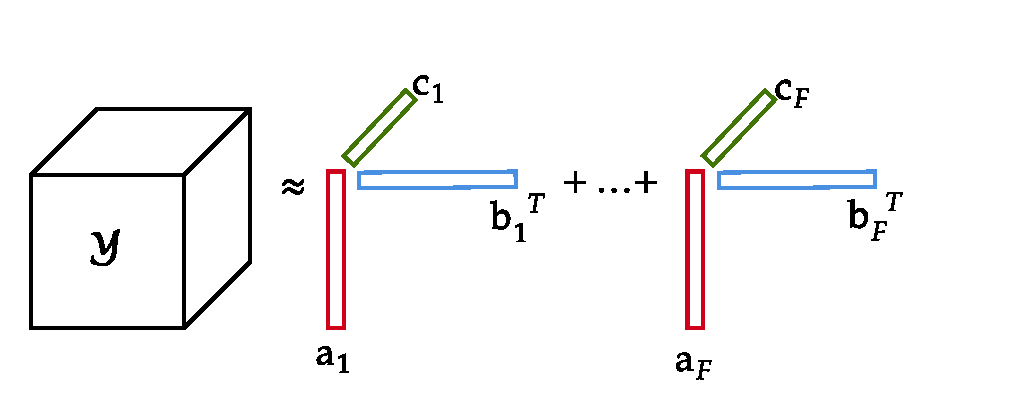
\includegraphics[height=1.5cm]{figures/cp}
%\]
%
%\item Tucker: $IR_1+JR_2+KR_3 +R_1R_2 R_3 - R_1^2 - R_2^2 - R_3^2$ 
%\[
%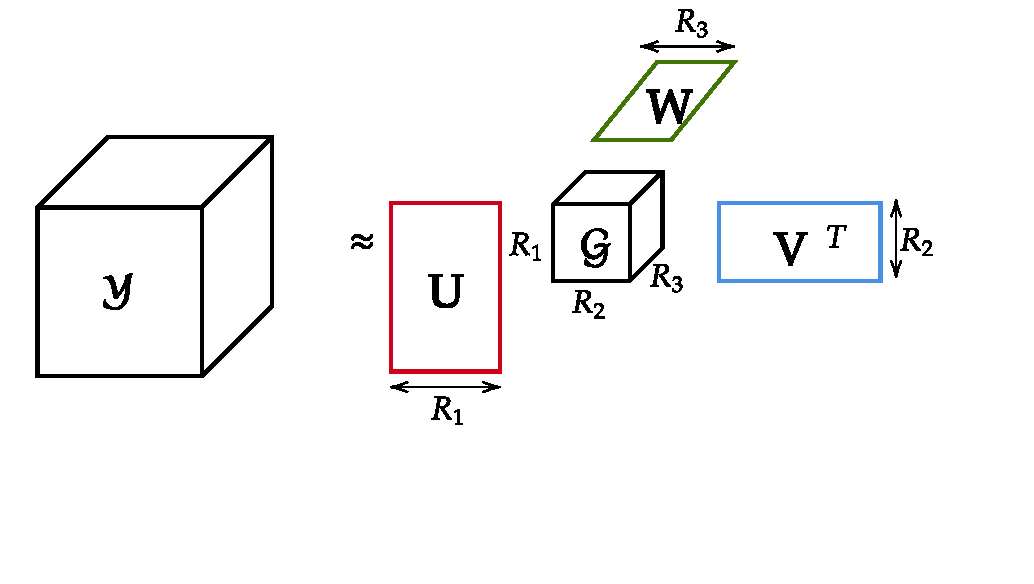
\includegraphics[height=2.5cm]{figures/tucker}
%\]
%\vspace{-3em}
%\end{itemize}
%
%Usages principaux:
%\begin{itemize}
%\item Tucker: compression (meilleurs algorithmes  )
%\item CP: identification (grace à la propriéte d'\textbf{unicité})
%\end{itemize}
%
%\end{frame}
%
%
%%\section{Unicité}
%%
%%\begin{frame}
%%\frametitle{Unicité de la décomposition CP}
%%\begin{center}
%%
\includegraphics[width=5cm]{figures/keep-calm-and-be-unique-350}
%%\end{center}
%%\end{frame}
%%
%%
%%\begin{frame}{Cas matriciel}
%%\[
%%\raisebox{-0.35\height}{\begin{tikzpicture}[scale=0.8]
%%\draw(4.7,0.5) node (A) {$\mathbf{M}$};
%%\draw(4,0) rectangle (5.4,1);
%%
%%\draw(5.7,0.5) node (eq) {$=$};
%%\draw(6.25,0) rectangle (6.85,1.2); %node {A};
%%\draw(6.55,0.6) node (A) {$A$};
%%%\draw(5,0.5) node (eq) {\footnotesize$\quad+\,\cdots\,+\quad$};
%%\draw(7,0.65) rectangle (8.2,1.2); %node {A};
%%\draw(7.6,0.95) node (A) {$B^{T}$};
%%
%%\draw(8.5,0.5) node (eq) {$=$};
%%\draw(8.75,0) rectangle (9.35,1.2); %node {A};
%%\draw(9.05,0.6) node (A) {$A$};
%%%%\draw(5,0.5) node (eq) {\footnotesize$\quad+\,\cdots\,+\quad$};
%%\draw(10.9,0.65) rectangle (12.1,1.2); %node {A};
%%\draw(11.5,0.95) node (A) {$B^{T}$};
%%
%%\draw(9.5,0.65) rectangle (10.05,1.2); %node {A};
%%\draw(10.2,0.65) rectangle (10.75,1.2); %node {A};
%%
%%
%%\draw(9.75,0.925) node (A) {\Red{\small $S$}};
%%\draw(10.5,0.975) node (A) {\Red{\small $S^{\text{-}1}$}};
%%\end{tikzpicture}}
%%\]
%%indétermination: ordre, échelle, rotation
%%
%%
%%\vspace{1em}
%%
%%Pas d'unicité sans contraintes (e.g. nonnegativité dans NMF).
%%\end{frame}
%%
%%
%%
%%\begin{frame}\frametitle{Unicité essentielle}
%%
%%
%%\textbf{Unicité essentielle} : aux indéterminations d'ordre et d'échelle près.
%%$$
%%[\![\mathbf{A}, \mathbf{B}, \mathbf{C}]\!] = [\![\mathbf{A}\bm{\Pi} \bm{\Delta_A}, \mathbf{B}\bm{\Pi} \bm{\Delta_B}, \mathbf{C}\bm{\Pi} \bm{\Delta_C}]\!]
%%$$ 
%%avec
%%\begin{itemize}
%%\item $ \bm{\Pi}$ : matrice de permutation 
%%\item $\bm{\Delta_A},\ \bm{\Delta_B}, \ \bm{\Delta_C}$ : matrices diagonales telles que $\bm{\Delta_A} \bm{\Delta_B} \bm{\Delta_C} = \mathbf{I}$
%%\end{itemize}
%%
%%\[
%%\updownarrow
%%\]
%%
%%
%%Permutation et changement d'échelle de termes de rang 1
%%\[
%%\calX = \bfa_1 \circ \bfb_1 \circ \bfc_1 + \cdots+ \bfa_R \circ \bfb_R \circ \bfc_R = \sum\limits_{r=1}^{R} \frac{1}{\alpha_r\beta_r\gamma_r}(\alpha_r\bfa_r) \circ (\beta_r\bfb_r) \circ (\gamma_r\bfc_r) 
%%\]
%%\end{frame}
%%
%%\begin{frame}\frametitle{Theorème de Kruskal}
%%\textbf{Rang de Kruskal }$k_{\mathbf{A}}$ : valeur maximale de $k$ telle que toute sélection de $k$ colonnes de $\mathbf{A}$ forme une famille libre ($k_{\mathbf{A}} \leq r_{\mathbf{A}} = \text{rang }\mathbf{A}$).
%%\\[2ex]
%%Remarque : $\text{spark}(\mathbf{A}) = k_{\mathbf{A}}+1$
%%\\[2ex]
%%\textbf{Exemples} :
%%$$
%%\mathbf{A}= [ 
%%    \mathbf{a}_1  \quad  \mathbf{a}_2  \quad \mathbf{a}_3 \quad \mathbf{a}_4 ]
%%$$
%%
%%$$
%%\mathbf{A}= [\mathbf{a}_1 \quad \mathbf{a}_1 \quad \mathbf{a}_3  \quad \mathbf{a}_4]
%%$$
%%
%%$$
%%\mathbf{A}= [\mathbf{a}_1 \quad \mathbf{a}_2  \quad \mathbf{a}_1+ \mathbf{a}_2 \quad \mathbf{a}_4]
%%$$
%%
%%\textbf{Condition de Kruskal} : si  $k_{\mathbf{A}},  k_{\mathbf{B}}, k_{\mathbf{C}} \geq 2$ et $k_{\mathbf{A}} + k_{\mathbf{B}} + k_{\mathbf{C}} \geq 2 R +2 $, alors $[\![\mathbf{A}, \mathbf{B}, \mathbf{C}]\!] $ est essentiellement unique $[$Kruskal, 1977$]$.
%%\\[2ex]
%%Si $k_{\mathbf{A}}=1$, modèle non identifiable
%%
%%\end{frame}
%%
%%
%%
%%\begin{frame}\frametitle{Condition de Kruskal}
%%\[
%%k_{\mathbf{A}} + k_{\mathbf{B}} + k_{\mathbf{C}} \geq 2 R +2 
%%\]
%%\begin{itemize}
%%\item \textbf{Cas d'une matrice de rang colonne plein} : si $\mathbf{C}$ est de rang colonne plein et que les matrices $\mathbf{A}$ et $\mathbf{B}$ satisfont  1) $k_{\mathbf{A}},  k_{\mathbf{B}}  \geq 2$ et 2)
%%$ r_{\mathbf{A}} + k_{\mathbf{B}} \geq  R +2 $ ou $ r_{\mathbf{B}} + k_{\mathbf{A}} \geq  R +2 $ alors  $[\![\mathbf{A}, \mathbf{B}, \mathbf{C}]\!] $ est essentiellement unique $[$Guo, 2011$]$.
%%\item Conditions d'identifiabilité partielle $[$Guo et al., 2013$]$ (unicité d'un des facteurs).
%%\item
%%\textbf{Identifiabilité générique } (tenseur cubique) : si $\mathbf{A}$, $\mathbf{B}$ et $\mathbf{C}$ sont des matrices dont les valeurs sont des réalisations de v.a. à densité absolument continue et dont les dimensions sont telles que $I, \ J , \ K$ alors $[\![\mathbf{A}, \mathbf{B}, \mathbf{C}]\!] $ est essentiellement unique si $R \leq \lceil \frac{I^3}{3I-2}\rceil$  $[$Lickteig, 1986$]$ (extensions pour le cas non-cubique: $[$Chiantini et al., 2015$]$).
%%\end{itemize}
%%
%%\textbf{\color{blue} Matlab (demo 3) }
%%\end{frame}
%
%
%\section{Applications}
%
%\begin{frame}
%\frametitle{Example en chimiometrie (MEEF)}
%\uncover<4>{
%\[
%\begin{array}{l} 
%\text{spectroscopie de fluorescence} \\
%\text{matrice d'Emission/Excitation } \\
%\end{array}\quad
%\begin{array}{c} 
%\text{ \Red{rang = \# composants} de mélange} \\
%\text{$N$ experimentations, \Blue{concentrations différentes}} \\
%\end{array}
%\]}
%\[
%\begin{array}{c@{}l}
%\text{\uncover<4->{\raisebox{-0.45\height}{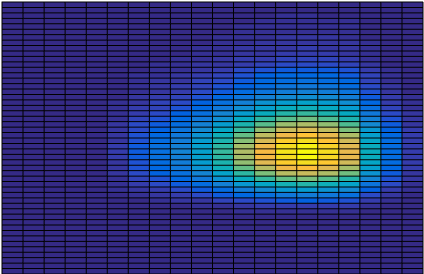
\includegraphics[height=1.2cm]{figures/2dspectrum1}} = }} & 
%\raisebox{-0.35\height}{\begin{tikzpicture}
%\draw<1>(0,0.5) node (A) {$\mathbf{M}_{\phantom{1}}$};
%\draw<2->(0,0.5) node (A) {$\mathbf{M}_1$};
%\draw(-0.7,0) rectangle (0.7,1);
%\draw(1.1,0.5) node (eq) {${=}$};
%\draw(1.7,0) -- (1.7,1);
%\draw(1.7,0.5) node[fill=white] (a1) {{ $\bfa_1$}};
%\draw(1.8,1) -- (3.18,1);
%\draw(2.45,1) node[fill=white] (b1) {{\small $\bfb_1^{\T}\!\!$}};
%\draw(3.5,0.5) node () {{\small $+\; \cdots\;+$}};
%\draw(4.7,0) -- (4.7,1);
%\draw(4.7,0.5) node[fill=white] (a1) {{ $\bfa_r$}};
%\draw(4.8,1) -- (6.18,1);
%\draw(5.45,1) node[fill=white] (b1) {{\small $\bfb_r^{\T}\!\!$}};
%
%\draw<2->(1.4,1.05) node (eq) {{ $\Blue{c_{1,1}}\cdot$}};
%\draw<2->(4.4,1.05) node (eq) {{ $\Blue{c_{r,1}}\cdot$}};
%\end{tikzpicture}} \\
%\uncover<4->{\vdots}& \qquad\uncover<2->{\vdots} \\
%\text{\uncover<4->{{\raisebox{-0.45\height}{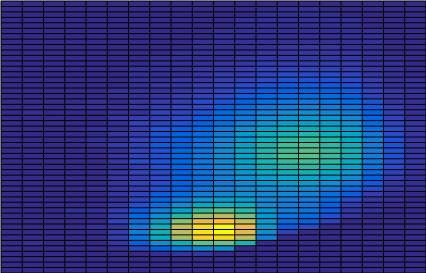
\includegraphics[height=1.2cm]{figures/2dspectrum2}}} = }} & 
%\uncover<2->{\raisebox{-0.35\height}{\begin{tikzpicture}
%\draw(0,0.5) node (A) {$\mathbf{M}_N$};
%\draw(-0.7,0) rectangle (0.7,1);
%\draw(1.1,0.5) node (eq) {${=}$};
%\draw(1.7,0) -- (1.7,1);
%\draw(1.7,0.5) node[fill=white] (a1) {{ $\bfa_1$}};
%\draw(1.8,1) -- (3.18,1);
%\draw(2.45,1) node[fill=white] (b1) {{\small $\bfb_1^{\T}\!\!$}};
%\draw(3.5,0.5) node () {{\small $+\; \cdots\;+$}};
%\draw(4.7,0) -- (4.7,1);
%\draw(4.7,0.5) node[fill=white] (a1) {{$\bfa_r$}};
%\draw(4.8,1) -- (6.18,1);
%\draw(5.45,1) node[fill=white] (b1) {{\small $\bfb_r^{\T}\!\!$}};
%\draw<2->(1.35,1.05) node (eq) {{ $\Blue{c_{1,N}}\cdot$}};
%\draw<2->(4.35,1.05) node (eq) {{ $\Blue{c_{r,N}}\cdot$}};
%\end{tikzpicture}}} \\
%& \qquad\qquad\;\; \uncover<3->{\Updownarrow} \\
%& \uncover<3->{\!\!\!\!\raisebox{-0.3\height}{\begin{tikzpicture}
%\begin{scope}[scale= 0.5]
%%\draw(0.5,0.5) node (A) {$\mathcal{T}$};
%%\draw(0,0) rectangle (1,1);
%%\draw(0,1) -- (0.5,1.5) -- (1.5,1.5) -- (1.5,0.5) --(1,0);
%%\draw(1,1) -- (1.5,1.5);
%\draw[fill=white](-0.5,0.88) rectangle (1.5,2.5);
%\draw[fill=white](-1.5,-0.12) rectangle (0.5,1.5);
%%\draw[fill=white](-0.75,-0.75) rectangle (1.25,1.25);
%\draw[fill=white](-2,-0.7) rectangle (0,0.92);
%\draw(-1,0.7) node (A) {\small $\bfM_1$};
%\draw(-0.5,1.25) node (B) {\small $\bfM_2$};
%\draw(0.5,2.25) node (C) {\small $\bfM_N$};
%\draw(-0.95,2.15) node (D) {\small $\iddots$};
%
%
%
%\draw(2.1,0.8) node (eq) {$=$};
%\draw(6.8,0.8) node (eq) {$\quad+\,\cdots\,+\quad$};
%\end{scope}
%
%\begin{scope}[scale= 0.5,xshift=1.4cm]
%\draw(2,-0.2) -- (2,0.8);
%\draw(2.1,0.3) node[anchor=east] (s21) {\small {$\bfa_1$}};
%\draw(2.2,1) -- (4,1);
%\draw(3.0,1.2) node[anchor=north] (s22) {\small {$\bfb_1$}};
%\draw(2.2,1.2) -- (3.2,2.2);
%\draw(2.7,1.3) node[anchor=south east] (s23) {\small{$\bfc_1$}};
%\end{scope}
%
%\begin{scope}[scale= 0.5,xshift=7.3cm]
%\draw(2,-0.2) -- (2,0.8);
%\draw(2.1,0.3) node[anchor=east] (s21) {\small {$\bfa_r$}};
%\draw(2.2,1) -- (4,1);
%\draw(3.0,1.2) node[anchor=north] (s22) {\small {$\bfb_r$}};
%\draw(2.2,1.2) -- (3.2,2.2);
%\draw(2.7,1.3) node[anchor=south east] (s23) {\small {$\bfc_r$}};
%%\draw(1.9,1) node (g1) {\textcolor{red}{\small $c_r$}};
%\end{scope}
%\end{tikzpicture}}}\\
%\end{array}
%\]
%\end{frame}
%
%\begin{frame}{Exemple: classification d'images}
%\textbf{Réseau convolutionnnel}
%\[
%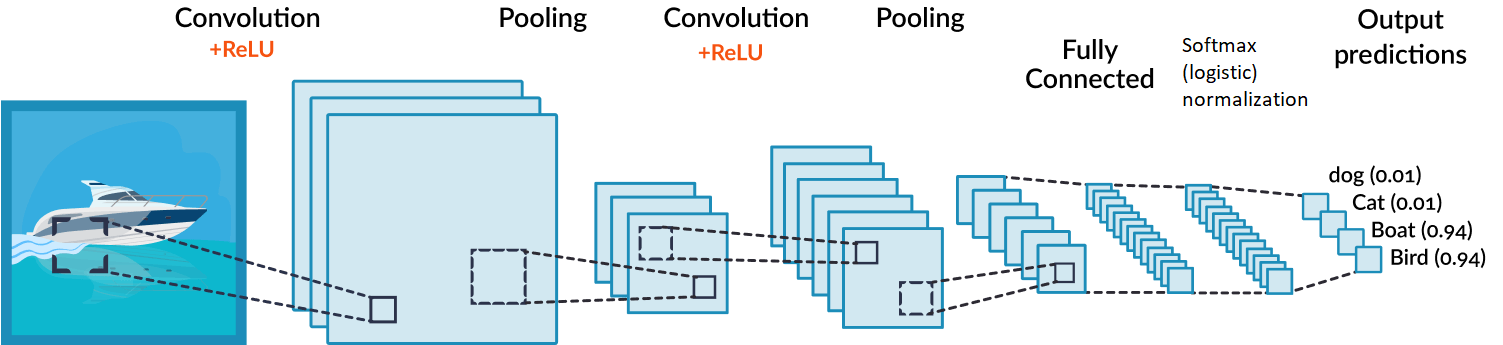
\includegraphics[height=2.5cm]{figures/convnet.png}
%\]
%
%\begin{itemize}
%\item Inconvenient: cout important de stockage
%\end{itemize}
%
%\end{frame}
%
%
%
%\begin{frame}{Convolutional layers}
%\[
%\raisebox{-0.5\height}{\begin{tikzpicture}
%\begin{scope}[scale=0.6]
%\draw[fill=white](1,1) rectangle (3,3);
%\draw[fill=white](-0.5,-0.5) rectangle (1.5,1.5);
%\draw[fill=white](-1,-1) rectangle (1,1);
%
%\draw(0,0) node (A) {$\tens{U}$};
%\draw(0.5,1.25) node (B) {};
%\draw(2,2.75) node (C) {};
%\draw(0.5,2) node (D) {\small $\iddots$};
%
%\draw(0,-1.25) node (D) {\small $J$};
%\draw(-1.25,0) node (D) {\small $I$};
%\draw(0,2.5) node[rotate=45] (D) {\small $S$ input features};
%\end{scope}
%\end{tikzpicture}}
%\quad
%\xrightarrow{\substack{\text{convolution avec $T$}\\ \text{$(d\times d\times S)$ filtres 2D}} }
%\quad
%\raisebox{-0.5\height}{\begin{tikzpicture}
%\begin{scope}[scale=0.6]
%\draw[fill=white](1,1) rectangle (3,3);
%\draw[fill=white](-0.5,-0.5) rectangle (1.5,1.5);
%\draw[fill=white](-1,-1) rectangle (1,1);
%
%\draw(0,0) node (A) {$\tens{V}$};
%\draw(0.5,1.25) node (B) {};
%\draw(2,2.75) node (C) {};
%\draw(0.5,2) node (D) {\small $\iddots$};
%
%\draw(0,-1.25) node (D) {\small $J\text{-}d\!\!+\!\!1$};
%\draw(-1.8,0) node (D) {\small $I\text{-}d\!\!+\!\!1$};
%\draw(0,2.5) node[rotate=45] (D) {\small $T$ output features};
%\end{scope}
%\end{tikzpicture}}
%\]
%\begin{align*}
%\mathcal{V}(x,y,t) &= g\Big( \sum\limits_{i=x-d+1}^{x}\sum\limits_{j=y-d+1}^{y} \sum\limits_{s=1}^{S} \mathcal{K}(i-x+d, j-y+d,s,t) \mathcal{U}(i,j,s) \\
%& + b(x,y,t)\Big)
%\end{align*}
%défini par  tensor $4D$  $\tens{K} \in \RR^{d\times d \times S\times T}$
%
%\vspace{1em}
%
%$\Rightarrow$ compression par décomposition CP
%
%
%\end{frame}
%
%\begin{frame}{Tensor approximations for NN compression}
%\emph{\small (Lebedev et al., 2015)}
%\[
%\mathcal{K} \approx\sum\limits_{r=1}^{R} \bfa_r \circ \bfb_r \circ \bfc_r \circ \bfd_r , 
%\]
%\[
%\!\!\!\! \begin{array}{@{}ccc@{}}
%\text{full convolution} & & \text{sequence of 1D convolutions} \\ 
%\raisebox{-0.5\height}{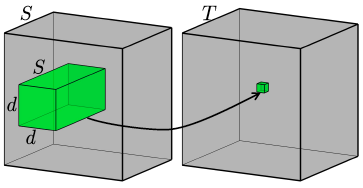
\includegraphics[height=1.6cm]{figures/conv_full.png}} &\to& \raisebox{-0.5\height}{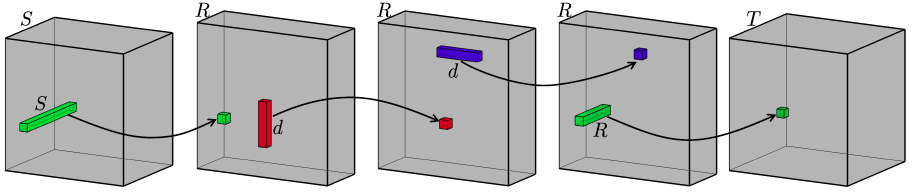
\includegraphics[height=1.6cm]{figures/conv_cpd.png}}
%\end{array}
%\]
%
%
%\end{frame}
%
%
%\begin{frame}
%\frametitle{Conclusion}
%
%\begin{itemize}[label=\tiny$\blacksquare$]
%	\item Les données se présentent très généralement sous forme matricielles/tensorielles
%	\item Nécessité de savoir manipuler ces structures
%	\item Il est important d'avoir des méthodes d'approximation/simplification de ces données. Cela passe souvent par des algoithmes de décompositions ou factorisations
%	\item Les propriétés mathématiques des décompositions (existence, unicité, etc..) influent sur la complexité du problème.
%\end{itemize}
%\end{frame}
%
%
\end{document}
% The log drawn in the upper right corner.
%\logo{\includegraphics[height=0.125\paperheight]{logo-telekinesis}}


